%%%%%%%%%%%%%%%%%%%%%%%%%%%%%%%%%%%%%%%%%%%%%%%%%%%%%%%%%%%%%%%%%%%%%%%%%%%%%%%%%%%%%%%%%%%%%%%%%%%%%
% This template is distributed with ABSOLUTELY NO WARRANTY.
% It serves as a guideline and constitutes a basic structure for a
% thesis/dissertation. The user assumes full responsibility for formatting
% and typesetting their document and for verifying that all the thesis
% requirements set by the University of Tennessee are met. Please refer to the most
% recent UT thesis guide (http://web.utk.edu/~thesis/thesisresources.shtml)
% or contact the thesis consultant (http://web.utk.edu/~thesis/).
% Please report any bugs to the thesis consultant.
%%%%%%%%%%%%%%%%%%%%%%%%%%%%%%%%%%%%%%%%%%%%%%%%%%%%%%%%%%%%%%%%%%%%%%%%%%%%%%%%%%%%%%%%%%%%%%%%%%%%%
% O P T I O N S:
% 1. thesis/dissertation
% 2. monochrome
% 3. all options provided by the report class
\documentclass[dissertation,letterpaper,12pt]{utthesis}
% some alternatives are:
%\documentclass[thesis,monochrome,letterpaper,12pt]{utthesis} %thesis, one side, monochrome text
%\documentclass[thesis,twoside,letterpaper,12pt]{utthesis} % thesis, two side
%\documentclass[thesis,monochrome,twoside,letterpaper,12pt]{utthesis} % thesis, two side, monochrome text
% for a dissertation, replace the thesis option by dissertation:
% \documentclass[dissertation,letterpaper,12pt]{utthesis} . . .
\renewcommand{\baselinestretch}{1.5} % line Spacing
%%%%%%%%%%%%%%%%%%%%%%%%%%%%%%%%%%%%%%%%%%%%%%%%%%%%%%%%%%%%%%%%%%%%%%%%%%%%%%%%%%%%%%%%%%%%%%%%%%%%%
% PROPOSAL METADATA
%%%%%%%%%%%%%%%%%%%%%%%%%%%%%%%%%%%%%%%%%%%%%%%%%%%%%%%%%%%%%%%%%%%%%%%%%%%%%%%%%%%%%%%%%%%%%%%%%%%%%
\title{Deep Learning for Biological Discovery Across Omics Layers: From Phenomics to Mechanistic Reasoning}	       % title of thesis/dissertation
\author{Peter Kruse}                % author's name
\copyrightYear{2026}            % copyright year of your thesis/dissertation
\graduationMonth{September}         % month of proposal
\majorProfessor{Dr. Daniel Jacobson}	    % advisor's nameb
\keywords{Systems Biology, Deep Learning, Genetics, Computer Vision, Large Language Models, Multi-Omics}	% keywords (optional) separated by commas - these are used in the PDF file properties
\viceProvost{Dixie L. Thompson} % vice provost name
\major{Data Science Engineering}					% major: Computer Science, Biology, Mathematics, ...
\degree{Doctor of Philosophy}	    			% degree: Doctor of Philosophy, Master of Science, Master of Arts, ...
\college{Intercollegiate}
\dept{Bredesen Center for Interdisciplinary Research and Graduate Education}
\university{The University of Tennessee, Knoxville}	% school name
% THIS TEMPLATE ACCOMMODATES UP TO 5 COMMITTEE MEMBERS - ENTER ONLY THE NAMES OF THE MEMBERS ON YOUR COMMITTEE
\numberOfCommitteeMembers{4} % enter the number of committee members
\committeeMemberA {Dr. Daniel Jacobson}	% name of committee chair
\committeeMemberB {Dr. Michael Langston}	% name of second committee member
\committeeMemberC {Dr. Katherine Schuman}	% third committee member
\committeeMemberD {Dr. Hairong Qi}	% fourth committee member
%%%%%%%%%%%%%%%%%%%%%%%%%%%%%%%%%%%%%%%%%%%%%%%%%%%%%%%%%%%%%%%%%%%%%%%%%%%%%%%%%%%%%%%%%%%%%%%%%%%%%
% LOAD SOME USEFUL PACKAGES
%%%%%%%%%%%%%%%%%%%%%%%%%%%%%%%%%%%%%%%%%%%%%%%%%%%%%%%%%%%%%%%%%%%%%%%%%%%%%%%%%%%%%%%%%%%%%%%%%%%%%
\usepackage{nomencl}                    % produces a nomenclature
\usepackage{float}                      % figure floats
\usepackage[T1]{fontenc}               % reliable accented text and small caps
\usepackage[utf8]{inputenc}
\usepackage{csquotes}                   % context-sensitive quotes; load before biblatex (provides displayquote)
\usepackage[style=numeric]{biblatex}
\addbibresource{references/references-dissertation.bib} 


\usepackage{graphicx}					% graphics package
\graphicspath{ {figures/}{figures/eps/}{figures/pdf/} }% specify the path where figures are located
\usepackage{fancyhdr}                   % fancy headers and footers
\usepackage{url}                        % nicely format url breaks
\usepackage[inactive]{srcltx}		 	% necessary to use forward and inverse searching in DVI
\usepackage{relsize}                    % font sizing hierarchy
\usepackage{booktabs}                   % professional looking tables
% \usepackage[config, labelfont={bf}]{caption,subfig} % removed: subfig clashes with subcaption (used for \begin{subfigure}); caption is loaded below
\usepackage{mathrsfs}                   % additional math scripts
\usepackage{setspace}
\usepackage{algorithm}                  % float wrapper for \begin{algorithm}
\usepackage{algpseudocode}              % algorithmicx pseudocode (\State, \For, ...); replaces old algorithmic
\usepackage{textcomp}
\usepackage{xcolor}
\usepackage[labelfont=bf]{caption}
\usepackage{subcaption}
\usepackage{hyperref}
% \usepackage{subfigure} % removed: deprecated, clashes with subcaption (\c@subfigure already defined); unused (no \subfigure{} commands)
\usepackage{tabularx}
\usepackage{longtable}
\usepackage{array}
\usepackage{makecell}                   % \makecell for multi-line table cells (chapter 3)
\newcolumntype{Y}{>{\raggedright\arraybackslash}X} % flexible text column (chapter 4 tables)

% --- review annotations -------------------------------------------------
% \todocite{description} marks a missing citation (red brackets). Never invent
% a citation key; use this instead.
\newcommand{\todocite}[1]{\textcolor{red}{[#1]}}

% \comment{note} is the channel for review notes in the source (blue, small
% sans, bracketed). Flip to \showcommentsfalse for a committee build; the notes
% stay in the source either way.
% number subsubsections so \ref to them resolves to its own number
\setcounter{secnumdepth}{3}

\newif\ifshowcomments
\showcommentsfalse
\newcommand{\comment}[1]{\ifshowcomments\textcolor{blue}{\textsf{\small\,[#1]}}\fi}
% ------------------------------------------------------------------------

% add a proposal title page edit
\makeatletter
\renewcommand{\makeTitlePage}{%
    \thispagestyle{empty}%
    \begin{spacing}{1.5}%
    \vspace*{0.3in}%
    \begin{center}%
        {\huge\bfseries \@title \par}%
        \vfill
        {\Large\rmfamily
            Comprehensive Exam\\[1.5em]
            \@university\\[1em]
            \@author\\[1em]
            \@graduationMonth\ \@copyrightYear%
            \par}%
    \end{center}%
    \end{spacing}%
    \cleardoublepage%
}
\makeatother

\def\BibTeX{{\rm B\kern-.05em{\sc i\kern-.025em b}\kern-.08em
    T\kern-.1667em\lower.7ex\hbox{E}\kern-.125emX}}
\captionsetup{justification=centering}
\setlength{\emergencystretch}{2em}

\hypersetup{
    colorlinks=true,
    linkcolor=blue,
    filecolor=blue,
    urlcolor=blue,
    citecolor=blue,
    % re-set the PDF document properties here: the class issues \hypersetup at
    % load time, before \title/\author/\keywords are defined, so it captures
    % the class placeholder values instead of these.
    pdftitle={Deep Learning for Biological Discovery Across Omics Layers: From Phenomics to Mechanistic Reasoning},
    pdfauthor={Peter Kruse},
    pdfsubject={Comprehensive Exam},
    pdfkeywords={deep learning, phenomics, genomic prediction, genotype-by-environment interaction, biological networks, reinforcement learning},
    pdfcreator={LaTeX with hyperref},
    } 
    
%%% PACKAGES THAT ARE PRELOADED WITH THE CLASS ARE: amsmath,amsthm,amssymb,setspace,geometry,hyperref,and color
%%%%%%%%%%%%%%%%%%%%%%%%%%%%%%%%%%%%%%%%%%%%%%%%%%%%%%%%%%%%%%%%%%%%%%%%%%%%%%%%%%%%%%%%%%%%%%%%%%%%%
\begin{document}
    \pagenumbering{alph} % this is needed to clear certain issues with the hyperref package
    \addToPDFBookmarks{0}{Front Matter}{rootNode} % create a root node named "Front Matter" in the pdf bookmarks
    \addToPDFBookmarks{1}{Title}{a} % add a pdf bookmark to the title page
    \makeTitlePage % make the title page. Make sure you properly set the \docType
    %
    \pagenumbering{roman}
    \setcounter{page}{2}
    %
    \makeCopyrightPage % make the copyright page 
    %
    \addToPDFBookmarks{0}{Table of Contents}{f}
    \tableofcontents % generate a table of contents
    %
    \addToTOC{List of Tables} % this will add the list of tables to the Table of Contents (TOC)
    \listoftables % generate a list of tables
    %
    \addToTOC{List of Figures} % this will add the list of figures to the Table of Contents (TOC)
    \listoffigures % generate a list of figures
    %
    \makenomenclature % OPTIONAL
    \addToPDFBookmarks{0}{Nomenclature}{g} % OPTIONAL
    \printnomenclature[1.25in] % OPTIONAL
    %
    \newpage
    \pagenumbering{arabic}
    \setcounter{page}{1}
    %%%%%%%%%%%%%%%%%%%%%%%%%%%%%%%%%%%%%%%%%%%%%%%%%%%%%%%%%%%%%%%%%%%%%%%%%%%%%%%%%%%%%%%%%%%%%%%%%%%%%
    % INCLUDE THE CHAPTERS STARTING WITH THE NOMENCLATURE IF PRESENT
    %%%%%%%%%%%%%%%%%%%%%%%%%%%%%%%%%%%%%%%%%%%%%%%%%%%%%%%%%%%%%%%%%%%%%%%%%%%%%%%%%%%%%%%%%%%%%%%%%%%%%
    % Enter the list of nomenclature here.
% Entries print alphabetically by symbol. The optional [sort key] is used only
% where the literal symbol would sort badly under makeindex, which orders by
% ASCII and therefore places math and lowercase initials out of sequence.
% Grouped by theme below for maintenance; grouping does not affect the output.

% --- Deep learning architectures and training ---
\nomenclature{BPE}{Byte-pair encoding}
\nomenclature{CNN}{Convolutional neural network}
\nomenclature{DDP}{Distributed data parallelism}
\nomenclature{DPO}{Direct preference optimization}
\nomenclature{FSDP}{Fully-sharded data parallelism}
\nomenclature{GRPO}{Group-relative policy optimization}
\nomenclature{HPC}{High-performance computing}
\nomenclature{LLM}{Large language model}
\nomenclature[aLORA]{LoRA}{Low-rank adaptation}
\nomenclature{LSTM}{Long short-term memory}
\nomenclature{MDP}{Markov decision process}
\nomenclature{MLP}{Multilayer perceptron}
\nomenclature[aMOE]{MoE}{Mixture of experts}
\nomenclature{PEFT}{Parameter-efficient fine-tuning}
\nomenclature{PPO}{Proximal policy optimization}
\nomenclature{RL}{Reinforcement learning}
\nomenclature{RLHF}{Reinforcement learning with human feedback}
\nomenclature{RNN}{Recurrent neural network}
\nomenclature{SAM}{Segment Anything Model}
\nomenclature{SFT}{Supervised fine-tuning}
\nomenclature{TRPO}{Trust region policy optimization}
\nomenclature[aVIT]{ViT}{Vision transformer}
\nomenclature[aZERO]{ZeRO}{Zero Redundancy Optimizer}

% --- Benchmarks, metrics, and evaluation ---
\nomenclature{CCC}{Concordance correlation coefficient}
\nomenclature{ILSVRC}{ImageNet Large Scale Visual Recognition Challenge}
\nomenclature{IoU}{Intersection over union}
\nomenclature{LEO}{Leave-environment-out validation}
\nomenclature[aMIOU]{mIoU}{Mean intersection over union}
\nomenclature{MSE}{Mean squared error}
\nomenclature{PCC}{Pearson correlation coefficient}

% --- Genetics and genomic prediction ---
\nomenclature{EC}{Environmental covariate}
\nomenclature{G2F}{Genomes to Fields}
\nomenclature{GAPIT}{Genome Association and Prediction Integrated Tool}
\nomenclature{GBLUP}{Genomic best linear unbiased predictor}
\nomenclature{GWAS}{Genome-wide association study}
\nomenclature[aGXE]{G$\times$E}{Genotype-by-environment}
\nomenclature[aH2]{$H^2$}{Broad-sense heritability}
\nomenclature{LD}{Linkage disequilibrium}
\nomenclature{MAF}{Minor allele frequency}
\nomenclature{MLM}{Mixed linear model}
\nomenclature{MLMM}{Multi-locus mixed model}
\nomenclature{SNP}{Single-nucleotide polymorphism}
\nomenclature{SNV}{Single nucleotide variant}
\nomenclature{TAV2}{Pennycress (\textit{Thlaspi arvense}) version 2 reference genome}

% --- Network biology and mechanistic interpretation ---
\nomenclature{GO}{Gene Ontology}
\nomenclature{GRIN}{Gene set Refinement through Interacting Networks}
\nomenclature[aIRFLOOP]{iRF-LOOP}{Iterative Random Forest Leave-One-Out Prediction}
\nomenclature{KEGG}{Kyoto Encyclopedia of Genes and Genomes}
\nomenclature{MDI}{Mean decrease in impurity}
\nomenclature{MENTOR}{Multiplex Embedding of Networks for Team-Based Omics Research}
\nomenclature{MENTOR-EV}{MENTOR applied with every gene in a multiplex as a seed, yielding a hierarchy over the full gene universe}
\nomenclature{MENTOR-IA}{MENTOR Interpretation Agent}
\nomenclature{MENTOR-RL}{The reinforcement learning-trained mechanistic reasoning model proposed in Chapter~\ref{ch4:mentor-rl}}
\nomenclature{PEN}{Predictive expression network}
\nomenclature{PPN}{Predictive phenotype network}
\nomenclature{RWR}{Random walk with restart}
\nomenclature{RWR-LOE}{Random walk with restart, lines of evidence}
\nomenclature{TAIR}{The Arabidopsis Information Resource}

% --- Imaging and color spaces ---
\nomenclature{CIELAB}{CIE $L^*a^*b^*$ color space; $a^*$ is the green--red axis and $b^*$ the blue--yellow axis}
\nomenclature{HSV}{Hue, saturation, value (brightness) color space}
\nomenclature{RGB}{Red, green, blue color space}

% --- Facilities ---
\nomenclature{OLCF}{Oak Ridge Leadership Computing Facility}

    \chapter*{Executive Summary}\label{ch:exec-sum}

\section{Motivation}
Modern biology has become increasingly data-rich but interpretation-limited. Data collection is now cost-effective in many realms, enabling the construction of novel datasets. High-throughput imaging technology has led to population-scale phenotyping datasets, while advanced sequencing methods allow researchers to capture genome-scale variation across populations. Global consortia efforts have standardized environmental metadata across climates and sites, while novel experimental data and computational frameworks have prompted the curation and creation of biological networks and large literature corpora. These data span fundamentally different structures: images contain spatial, pixel-level information; genotypes comprise high-dimensional, sparse signals; environments exist in a continuous and contextual space; and networks represent relational graph structures. Handling these different structures requires systems with different inductive biases; no single model class can handle them all.

\section{Thesis Statement}
While progress has been made applying deep learning to localized areas, biological data are heterogeneous and structurally varied, making the gains from current deep learning methods unequally distributed. Because of the nature of biological data, bridging the gap between inputs and interpretation requires problem-specific systems. Architectures, objectives, and benchmarks must be designed with appropriate inductive biases. This proposal demonstrates the utility of this framework across three linked stages of biological discovery: \textit{measurement}, \textit{prediction}, and \textit{interpretation.}

\section{Chapter 2 Summary}
Chapter 2 addresses the \textit{measurement} stage by extracting quantitative phenotypes from raw imagery. No deep learning framework currently exists for phenotyping pennycress (\textit{Thlaspi arvense L.}), an emerging oilseed cover crop. In this work, we present an automated deep learning pipeline that extracts 52 tissue-resolved phenotypes per seed pod. We benchmarked convolutional, transformer, and foundation-model segmentation architectures using 347 manually annotated pods from 21 scans, including an independent test set of 65 pods. A boundary-down-weighted U-Net achieved 85.58\% mean intersection over union while offering the most favorable accuracy--efficiency tradeoff. We then applied the pipeline to 12,253 seed pods from 768 accessions and connected the resulting trait matrix to candidate genetic mechanisms through heritability filtering, genome-wide association, network-based gene pruning, module construction, and expression analysis.

\section{Chapter 3 Summary}\label{sec:ch3}
Chapter 3 addresses the \textit{prediction} stage by mapping genotype and environment to phenotype. Accurate maize yield prediction is crucial for global food security, but remains challenging due to complex genotype-by-environment (G$\times$E) interactions. In this work, we present a unified transformer architecture for maize yield prediction that places 2,224 single-nucleotide variant markers and 702 environmental covariates in one sequence, allowing self-attention to learn direct G$\times$E interactions. A sparse mixture-of-experts layer supports token-level specialization, and an environment-conditioned affine head calibrates absolute yield while preserving within-environment rank. We trained on 143,050 usable pre-2024 Genomes2Fields plot records from 238 environments and retrospectively evaluated 9,486 records from 22 environments in the 2024 competition cohort. The selected model achieved a macro environment Pearson correlation coefficient of 0.423 and mean squared error of 55.40, corresponding to sixth place in the retrospective competition comparison and approaching the winning correlation of 0.45.

\section{Chapter 4 Summary}\label{sec:ch4}
Chapter 4 addresses the \textit{interpretation} stage by reasoning over biological networks to produce evidence-grounded mechanistic hypotheses. We propose \textsc{Mentor-RL}, an open-weight model trained on an ontology-grounded lattice of context-specific multiplex networks. A world-model curriculum teaches three co-equal structural views---random-walk neighborhoods, network hierarchies, and connectivity---before direct preference optimization and reinforcement learning train a tool-using policy with deterministic, schema-grounded rewards. Two flagship tasks test whether the model can generate a hierarchy for an unseen context and project a target neighborhood onto that hierarchy while recovering the network connections the hierarchy suppresses. Feasibility experiments demonstrate full fine-tuning of gpt-oss-120b on up to 128 Frontier nodes and an end-to-end trajectory loop. In preliminary S0 mapping experiments, atomic tokenization increased overall hard-subset accuracy from 45.6\% to 85.9\%, with both mapping directions reaching 100\% on the tested subset.

\section{Completion Plan and Expected Outputs}
Chapters 2 and 3 are being prepared for journal submission, while Chapter 4 defines the proposed remaining research and its staged evaluation plan. The Chapter 3 model and Chapter 4 feasibility experiments use distributed training on the OLCF Frontier supercomputer \cite{frontier}. Upon publication, we will release the open-source ground truth dataset of hand-annotated seed pod images and segmentation pipeline (Chapter~\ref{ch2:pennycress}); the training and evaluation code (Chapter~\ref{ch3:gxe}); and the training environment, evaluation harness, and trained checkpoints across pipeline stages (Chapter~\ref{ch4:mentor-rl}).

    \chapter{Literature Review} \label{ch1:lit-review}

\section{Deep Learning History}

According to Goodfellow et al., the history of neural network research can be divided into three eras: cybernetics, connectionism, and deep learning~\cite{Goodfellow-et-al-2016}. In the following sections, we adopt this organizational structure to explore the development of deep learning.

\begin{figure}
    \centering
    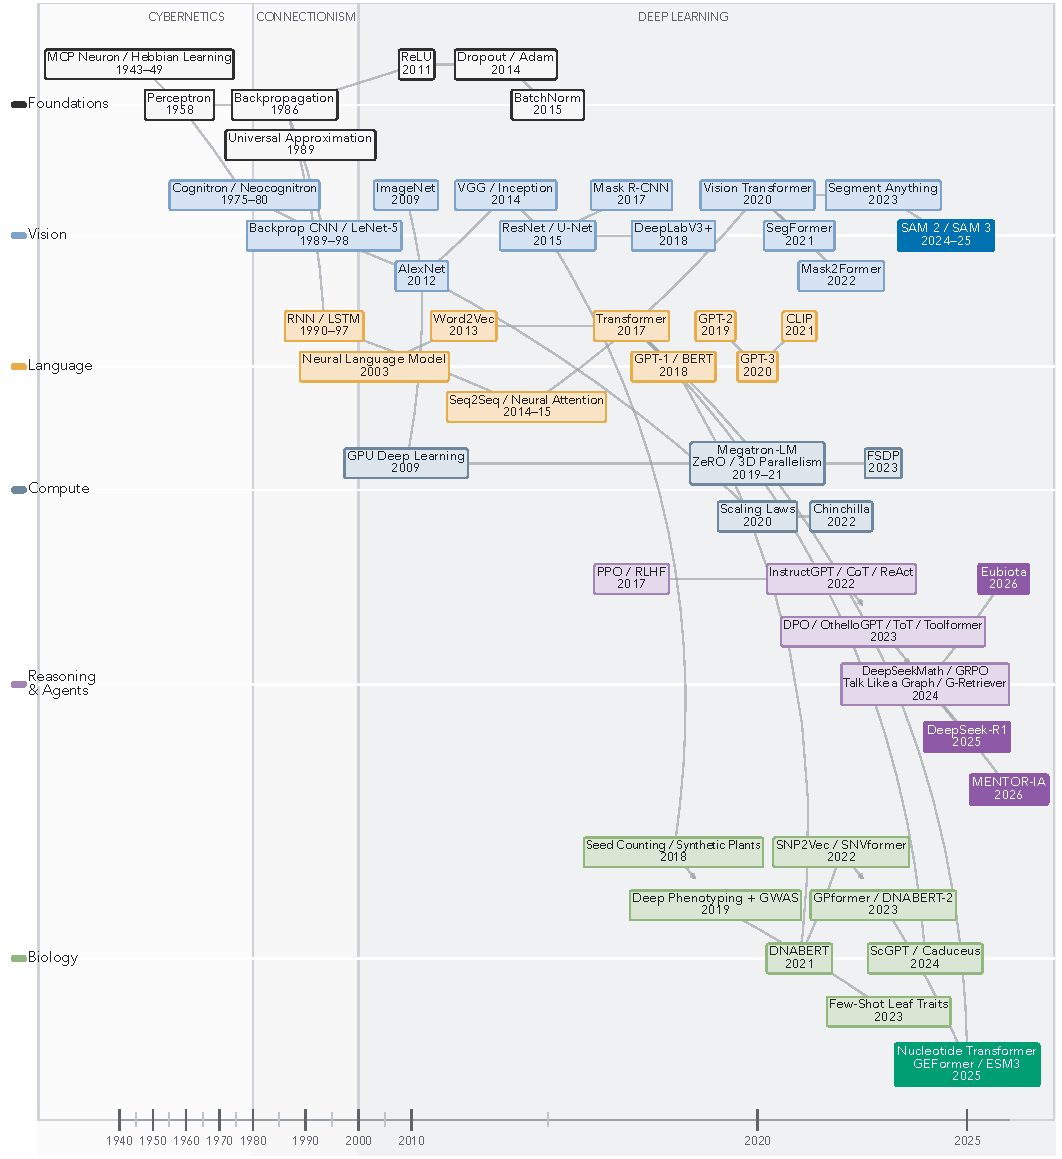
\includegraphics[width=\linewidth]{figures/lit-review/dl-timeline.pdf}
    \caption{History of Deep Learning (1940-2026)}
    \label{fig:ch1-dl-timeline}
\end{figure}


\subsection{Cybernetics}\label{sec:ch1-cybernetics}
The cybernetics era, spanning the 1940s and 1960s, was characterized by early efforts to formalize neural computation through the mathematical modeling of biological nervous systems. The first foundational contribution from this period was presented by McCulloch and Pitts in \textit{A Logical Calculus of Ideas Immanent in Nervous Activity}~\cite{mcculloch1943logical}. The authors provided a modeling framework for neuronal activity through the lens of formal logic; each neuron was framed as a binary computational unit within a larger symbolic logic network. Neuronal activation was determined by inputs corresponding to excitation and inhibition; an output was produced when the aggregated inputs exceeded a fixed threshold. Neurons emitted discrete logical outputs $True$ or $False$, enabling the construction of networks that implemented logical functions. Through this connected framework, McCulloch and Pitts aimed to model neural circuitry in the brain. Importantly, they emphasized that these networks worked over discrete time steps \textit{t}, allowing them to represent sequential dynamics and foreshadowing later concepts like recurrence and memory in neural systems.

Despite establishing a foundational framework for neural computation, the McCulloch-Pitts model exhibited several fundamental limitations. Most notably, the formulation lacked a learning mechanism: network structure and parameters were fixed, requiring manual design rather than learning from data. This static framework stood in contrast to Donald Hebb's work on synaptic plasticity, which postulated that neural pathways are strengthened by repeated co-activation~\cite{hebb1949organization}. Without such a mechanism, the behavior of the McCulloch-Pitts networks could not be modified in response to novel stimuli, limiting this framework's utility for modeling adaptive biological or cognitive processes. 

Furthermore, relying on a purely logical formulation imposed strict representational constraints. Neurons were restricted to binary activation states, resulting in rigid decision boundaries and precluding the learning of continuous representations. Together, these limitations prevented the McCulloch-Pitts networks from scaling to tasks requiring robust function approximation and learning from noisy, high-dimensional data.

The limitations of the McCulloch-Pitts neuron motivated subsequent efforts to develop neural models capable of adaptation, most notably Frank Rosenblatt's 1958 work \textit{The Perceptron: A Probabilistic Model for Information Storage and Organization in the Brain}~\cite{rosenblatt1958perceptron}. Rosenblatt described the perceptron as ``a hypothetical nervous system,'' reflecting an effort to maintain biological inspiration while introducing mechanisms for experience-driven learning. In contrast to the symbolic logic-based formulation of McCulloch and Pitts, Rosenblatt adopted a probabilistic perspective. He argued that the extensive assumptions and structure imposed by their model limited its ability to yield meaningful biological insight. Instead, the perceptron implemented a paradigm that treated data as statistically separable, with a learning mechanism that allowed connections to be reinforced or discouraged via positive or negative stimuli from the data.

While innovations introduced by the perceptron, such as trainable neurons and learning from data, are central to modern deep learning models, the original model had significant shortcomings. Most notably, Rosenblatt's formulation was incapable of representing non-linearly separable functions, with the XOR problem serving as a canonical example. This limitation was a consequence of the perceptron's reliance on linear decision boundaries and its restriction to single-layer architectures, and it severely limited its expressivity. Additionally, Rosenblatt's training rules could not be extended to multi-layer networks due to the lack of a credit assignment mechanism across multiple layers of computation. Combined with the use of binary outputs, these constraints severely limited the functions and representations that could be learned. 

These limitations were rigorously analyzed by Minsky and Papert in their 1969 book \textit{Perceptrons}, whose formal results played a significant role in altering public perception of AI research and contributed to a temporary decline in funding.

%% ADD FIGURE SHOWING THE XOR PROBLEM

\subsection{Connectionism}\label{sec:ch1-connectionism}
Although Minsky and Papert's work provided a rigorous exploration of the limitations of single-layer perceptrons, their critique did not explore whether such constraints could be overcome by multi-layer networks equipped with a credit assignment mechanism. The subsequent era of neural network research, commonly referred to as \textit{connectionism}, was defined by the efforts to address this challenge through the development of multi-layer architectures and the backpropagation algorithm. During this period neural networks also transitioned from primarily symbolic and biologically motivated abstractions toward increasingly general-purpose learning systems. As learning algorithms became more complex and models increased in scale, research increasingly began to favor mathematical tractability over biological interpretability~\cite{rumelhart1986learning, Goodfellow-et-al-2016}.

In 1986, Rumelhart, Hinton, and Williams published \textit{Learning Representations by Back-Propagating Errors}~\cite{rumelhart1986learning}, demonstrating that multi-layer neural networks could be effectively trained through a general solution to the credit assignment problem. Although the mathematical foundations for efficiently computing gradients, known as reverse-mode automatic differentiation, had been previously derived by Seppo Linnainmaa~\cite{linnainmaa1970representation} and applied to neural networks by Paul Werbos~\cite{werbos2005applications}, Rumelhart, Hinton, and Williams popularized the method within the AI community.

The backpropagation algorithm is a gradient-based learning procedure that propagates error information from the network's output backward through successive layers, incrementally modifying each parameter. Using networks trained with backpropagation, the authors showed that non-linearly separable functions could be learned by multilayer networks without relying on hand-designed learning rules.

Backpropagation relies on the differentiability of both the loss function and the network's activation functions, which allow gradients with respect to all parameters to be computed efficiently via the chain rule. This formulation enabled learning signals to be propagated to all network layers, in contrast to earlier approaches like the perceptron, which required a manually specified learning procedure. The formulation of weight updates as an optimization problem allowed neural network training to be extended to more complex multilayer architectures. In addition to backpropagation, this work made several other contributions, such as an explicit learning rate, momentum-based updates, and gradient accumulation, all of which are core to modern neural network optimization.

Beyond their algorithmic contribution, Rumelhart, Hinton, and Williams provided a conceptual framework for understanding multilayer networks. They characterized networks as self-organizing systems that were capable of learning internal representations from data, positing that hidden units in multilayer networks encode features of increasing complexity as network depth increases. These concepts formed the basis of future work in representation learning and motivated the exploration of deeper network architectures to model more complex structures in data.

The representational capabilities of neural networks were mathematically substantiated in 1989, when Cybenko and Hornik et al. independently published proofs of the Universal Approximation Theorem. These works demonstrated that a feed-forward network with a single hidden layer and a finite number of neurons can approximate any continuous function on a compact set~\cite{hornik1989multilayer, cybenko1989approximation}. While Cybenko's work was restricted to networks utilizing sigmoidal activation functions, Hornik et al. extended this result, proving that universality holds for any bounded, non-constant, and monotonically increasing activation function. This work provided a definitive rebuttal to Minsky and Papert's critique of perceptrons~\cite{minsky69perceptrons}, confirming that the limitations they identified were specific to single-layer architectures.

Despite these contributions, connectionist-era neural networks exhibited several limitations relative to modern deep learning models. Most notably, training was restricted by computational resources available at the time, which limited model size and large-scale experimentation. Neural networks were trained on general-purpose central processing units (CPUs), making it impractical to explore deeper architectures or large datasets.

In addition to computational constraints, optimization challenges further limited the effectiveness of early multilayer networks. The authors noted that the backpropagation algorithm could fail in the presence of local minima. With too small a learning rate, weight updates are not enough to traverse the loss landscape toward the global minimum. Furthermore, due to the use of activations such as sigmoid and tanh, gradients could become saturated during backpropagation. Excessively large or small values would fall near the asymptote of these functions, leading to vanishingly small values. As such, the resulting gradients would be small, multiplicatively reducing the learning signal in successive layers. These limitations prevented networks from increasing in depth and learning more complex representations, prompting the development of new methods to overcome these challenges.

\subsection{Deep Learning}\label{sec:ch1-deeplearning}
The transition from connectionism to deep learning emerged from convergent improvements in data, hardware, and algorithms during the late 1990s and early 2000s. These innovations addressed fundamental challenges of the connectionist era, such as vanishing gradients, computational bottlenecks, and convergence failures. Consequently, training networks with more layers became feasible and effective, leading to the era of deep learning, a term popularized by Geoffrey Hinton in 2006~\cite{hinton2006fast}. The pursuit of depth was built on the theoretical foundations laid by Rumelhart, Hinton, and Williams, who demonstrated that hidden layers allow networks to learn more complex hierarchical representations.~\cite{rumelhart1986learning, lecun2015deep}.

A key innovation in the deep learning era was the shift from CPUs to Graphics Processing Units (GPUs). The physical architecture of the GPU is well-suited for homogeneous, parallelizable, and batched operations, specifically massive matrix multiplications central to neural network training. In 2009, Raina et al. published \textit{Large-Scale Deep Unsupervised Learning Using Graphics Processors}, in which they trained Deep Belief Networks (DBNs)~\cite{hinton2006fast} and sparse coding networks~\cite{olshausen1996emergence} using GPUs~\cite{raina2009large}. By storing parameters in the GPU's global memory, parallelizing homogeneous thread operations in stream processors, and using efficient scheduling to reduce overhead times, the authors were able to achieve up to a 72x speedup in DBN training and a 15x speedup in sparse coding training. This acceleration rendered previously intractable problems computationally feasible; the reduction in training time enabled the exploration of deeper architectures and larger datasets, expanding the frontier of neural network training.

In order to fully leverage the benefits of GPU acceleration for neural network training, large, annotated datasets were necessary to avoid overfitting and improve generalization. The earliest advances in dataset construction occurred in the image domain; in the early 2000s, the MNIST dataset of handwritten digits~\cite{lecun1998gradient} served as the benchmark for neural network training. However, this dataset comprised only 10 image classes within a narrow domain, meaning that models trained on this data failed to capture general image recognition capabilities. To overcome these limitations, datasets such as Caltech101~\cite{fei2004learning}, PASCAL VOC~\cite{everingham2010pascal}, and MSRC~\cite{shotton2006textonboost} were developed, providing a wider variety of images and classes for training general-purpose computer vision models. Despite containing more subject diversity than MNIST, these datasets were still relatively small and lacked intra-class variability, with images often being standardized and lacking occlusions, translations, and other perturbations. In 2009, a breakthrough was made with the development and release of the ImageNet dataset~\cite{deng2009imagenet}. The authors of ImageNet leveraged the increasing amount of data available on search engines and the advent of crowdsourcing platforms like Amazon Mechanical Turk to produce a dataset of 3.2 million annotated images following the hierarchical structure of WordNet~\cite{fellbaum1998wordnet}. The availability of large-scale datasets such as ImageNet encouraged the development of neural networks with more layers to capture increasingly abstract and general image representations. This paradigm shift was further catalyzed by the ImageNet Large Scale Visual Recognition Challenge (ILSVRC)~\cite{ILSVRC15}, which will be discussed further in Section~\ref{sec:ch1-imagenet}.

As hardware capabilities improved and massive datasets became available, several algorithmic innovations enabled researchers to train deeper, larger-scale models. One notable breakthrough was the rectified linear unit, or ReLU, which supplanted the sigmoid and hyperbolic tangent (tanh) activation functions that were previously standard~\cite{rumelhart1986learning, lecun1991efficient}. Although ReLU was first utilized in Fukushima's \textit{Cognitron} and \textit{Neocognitron} architectures~\cite{fukushima1975cognitron, fukushima1980neocognitron}, it became widely adopted only after Glorot et al. published \textit{Deep Sparse Rectifier Networks} in 2011~\cite{glorot2011deep}. Glorot et al. showed that ReLU was not only more biologically plausible than its counterparts but also empirically outperformed them in both computer vision and sentiment analysis, especially with deep architectures. ReLU activation enforced network sparsity by setting negative activations to zero and mitigated the vanishing gradient problem with strictly linear positive activations, preventing gradient saturation. 

To fully leverage these properties, weight initialization techniques became widely adopted in deep networks. Building on the work of Glorot and Bengio, who introduced `Xavier initialization' to control the activation variance in sigmoidal networks~\cite{glorot2010understanding}, He et al. introduced `He initialization' to account for the rectification nonlinearity of ReLU~\cite{he2015delving}. These innovations facilitated the training of significantly deeper networks, cementing ReLU as a foundational component of the deep learning era.

To address the generalization challenges posed by these high-capacity models, Srivastava et al. introduced dropout in 2014~\cite{srivastava2014dropout}. Although large datasets such as ImageNet were becoming available, many domains lacked access to millions of labeled training examples. Consequently, deep networks tended to overfit smaller datasets, fitting noise and exhibiting high variance. Dropout ameliorated this issue by regularizing the co-adaptations between neurons. Biologically inspired by sexual reproduction, which reduces complex co-adaptation to make genes more robust, dropout probabilistically removes neurons from the network during training. As a result, neurons in the network cannot co-adapt with each other and must instead learn to function with a randomly chosen sample of units. As the authors stated, ``Complex co-adaptations can be trained to work well on a training set, but on novel test data they are far more likely to fail than multiple simpler co-adaptations that achieve the same thing.'' The utility of dropout is two-fold: it can enforce sparsity and considerably improves generalization error. Due to these factors, dropout has been ubiquitous in state-of-the-art architectures throughout the deep learning era.

In addition to ReLU and dropout, Ioffe and Szegedy introduced batch normalization in 2015, which allowed networks to be further extended~\cite{ioffe2015batch}. The authors aimed to remedy internal covariate shift a phenomenon where the distribution of activations in hidden layers shifts continuously based on parameter updates in previous layers. To mitigate this, the authors proposed normalizing layer activations around the mini-batch mean and variance. They demonstrated that batch normalization accelerates training and acts as a regularizer while also achieving state-of-the-art performance across multiple deep learning benchmarks. While Santurkar et al. argued in 2018 that batch normalization helps optimization through smoothing the optimization landscape instead of reducing internal covariate shift~\cite{santurkar2018does}, the technique remains a standard component in modern deep neural networks, facilitating the learning of increasingly complex representations.

Along with the architectural changes that made deep learning possible, the Adaptive Moment Estimation (Adam) optimizer was introduced to make weight updates for deeper networks more efficient~\cite{kingma2014adam}. Adam utilizes the first and second moments of the gradients to compute adaptive learning rates for each weight with little additional computation. The authors liken the resulting update rule to a ``trust region'' method: because the effective step size is bounded by the learning rate, optimization is effectively constrained to a neighborhood where the gradient estimate remains reliable. This promotes stability when gradients are sparse or noisy, allowing for faster convergence. Consequently, Adam has become the primary choice of optimizer in modern deep learning models.

The deep learning era was marked by the confluence of hardware improvements, data availability, and algorithmic innovation. These three factors enabled researchers to explore deep architectures that were previously impossible to train. As depth increased, a major paradigm shift occurred: the transition from \textit{feature engineering} to \textit{feature learning}~\cite{lecun2015deep}. While prior approaches relied on hand-crafted features to structure data, deeper networks allowed for complex representations to be learned directly in latent space, deriving hierarchical features with backpropagation instead of by hand.

With this shift away from manual feature engineering, research focus turned toward architectural and algorithmic design, with inductive biases tailored to specific data modalities. Computer vision assumed translation invariance, while language models assumed sequentiality and contextual dependence. These inductive biases align closely with the properties of biological data, making the history and current state of deep learning across modalities crucial for applications in phenomics, genomics, and systems biology. The remainder of this review is organized as follows: we cover computer vision in Section~\ref{sec:ch1-computervision} and language modeling in Section~\ref{sec:ch1-llms}. We then explore the techniques used to scale neural networks to massive modern datasets in Section~\ref{sec:ch1-hpc}. We will conclude with a review of how these techniques are applied to various biological subdomains in Section~\ref{sec:ch1-biology}.

\section{Computer Vision}\label{sec:ch1-computervision}
Computer vision served as the primary proving ground for neural network techniques and architectures during the deep learning era. This domain was the first where deep learning achieved widespread consumer adoption~\cite{lecun1998gradient} and later surpassed human performance~\cite{he2015delving}. Breaking these performance plateaus shifted the perception of deep learning from an esoteric field into a rapidly evolving discipline with disruptive applications. This success was not accidental; rather, the alignment between the structure of image data and the inductive biases of neural architectures, specifically convolutional neural networks (CNNs), allowed deep learning models to excel at learning complex representations. By integrating translation invariance, local connectivity, and hierarchy into neural architectures, researchers created biologically inspired vision models, grounded in Hubel and Wiesel's model of the mammalian visual cortex~\cite{hubel1959receptive, hubel1962receptive}, validating the connection between biological and artificial vision.

Several factors catalyzed rapid advancement of deep learning. The first was the establishment of standardized benchmarks that promoted competition and innovation in the computer vision community. The PASCAL VOC challenge~\cite{everingham2010pascal}, and subsequently the ILSVRC~\cite{ILSVRC15}, provided annual venues to evaluate visual recognition algorithms. These datasets, distinguished by their massive scale and public availability, provided a robust stage to validate methods while fostering competition and connectivity. This created a feedback loop that encouraged research participation and innovation in computer vision, leading to rapidly dropping competition error rates (see Figure~\ref{fig:ch1-ilsvrc-error-rate}). Due to the challenging nature of the ILSVRC and its popularity, the competition also served as a ``test bed,'' where techniques that succeeded in the image domain became part of the standard toolkit for other deep learning subdomains, including biological modeling. Foundational methods widely adopted after their demonstration in the ILSVRC include GPU parallelism~\cite{krizhevsky2012imagenet}, residual connections~\cite{he2016deep}, and data augmentation techniques~\cite{krizhevsky2012imagenet}.

\begin{figure}
    \centering
    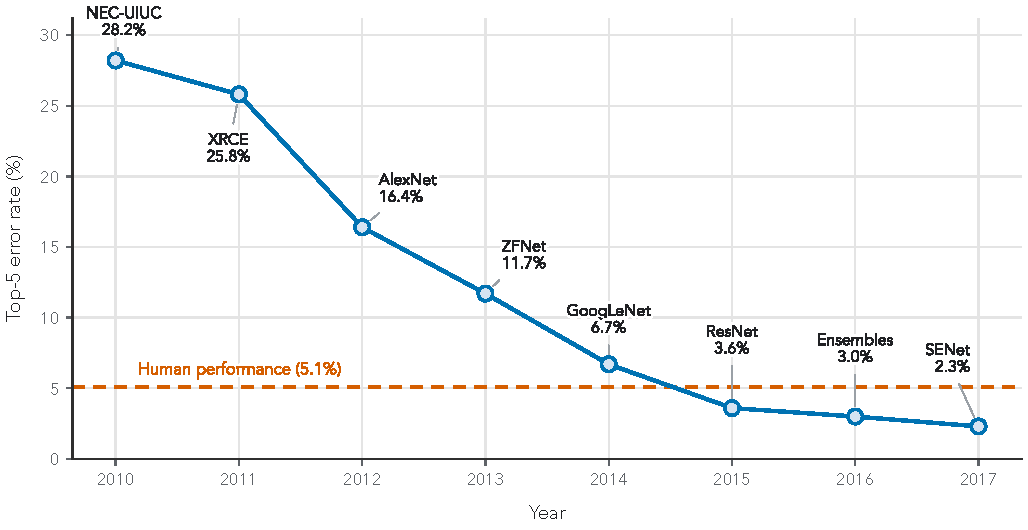
\includegraphics[width=\linewidth]{figures/lit-review/ilsvrc_error_rate_fixed.pdf}
    \caption{ILSVRC Top-5 Error Rate by Year (2010-2017)}
    \label{fig:ch1-ilsvrc-error-rate}
\end{figure}

The confluence of these factors enabled a transition from foundational benchmarking to biologically significant innovation. As performance on general image classification saturated, focus shifted to higher-order tasks, such as object detection, semantic segmentation, and automated feature extraction. These methodologies proved directly applicable to spatial and visual biological data, catalyzing innovation in image-based phenotyping, geospatial modeling, and multimodal artificial intelligence. Consequently, examining the evolution of computer vision is essential to understanding the technological development of modern biological modeling.

\subsection{Origins}\label{sec:ch1-origins}
Much like general deep learning research (Section~\ref{sec:ch1-cybernetics}), computer vision research began as a biologically inspired field grounded in neuroscience principles. In the late 1950s and early 1960s, Hubel and Wiesel provided the theoretical underpinnings for modern architectures with their work on the mammalian visual cortex~\cite{hubel1959receptive, hubel1962receptive}. They showed that vision is a hierarchical process built on detecting and combining local features. The visual cortex does not respond to the retinal input holistically; instead, neurons respond to stimuli within small, specific regions called receptive fields. Additionally, Hubel and Wiesel identified two types of cells involved in processing this visual information: simple cells and complex cells. While simple cells fire only when a specific feature, like a horizontal or vertical line, appears in a precise location, complex cells activate when the feature appears anywhere in the receptive field. Based on these fundamental units, they proposed a hierarchical model of visual processing: simple cells connect to complex cells, which connect to hypercomplex cells, allowing the visual cortex to build a layered representation that abstracts from lines to shapes and eventually to objects.

Kunihiko Fukushima built on this work by introducing the cognitron in 1975 and the neocognitron in 1980~\cite{fukushima1975cognitron, fukushima1980neocognitron}. A precursor to modern CNNs, the neocognitron operationalized the concepts of receptive fields, simple cells, and complex cells from Hubel and Wiesel. Instead of having fully connected layers like the perceptron~\cite{rosenblatt1958perceptron}, the neocognitron featured a shared weight mechanism. This simulated simple cells (referred to as ``S-cells'' by Fukushima) by applying the same filter to each part of the image, meaning a cell would activate any time its filter matched the input pattern in a region. Multiple S-cells could be applied to the image in parallel to detect multiple features. These features were then propagated to complex cells, or C-cells, for transformation-invariant feature detection. S-cells are equivalent to convolution operations, and C-cells are equivalent to pooling operations. The combination of multiple S-C layers resulted in a similar hierarchical structure to the model of visual processing introduced by Hubel and Wiesel~\cite{hubel1959receptive, hubel1962receptive}. Although Fukushima made foundational contributions to CNN architecture, the neocognitron relied on unsupervised competitive learning rather than backpropagation, which hindered its standalone success for complex supervised tasks.

In 1989, Yann LeCun combined the architectural foundations of Fukushima~\cite{fukushima1975cognitron, fukushima1980neocognitron} with the learning rules of Rumelhart et al.~\cite{rumelhart1986learning} to train the first modern CNNs~\cite{lecun1989handwritten}. LeCun used backpropagation to train a CNN for recognizing digits from the United States Postal Service. The model achieved a 1\% error rate and 9\% rejection rate, demonstrating state-of-the-art performance on a real-world task. This result showed that utilizing convolutions for computer vision tasks was a promising approach; because the model learned hierarchical features, the need for manual preprocessing was minimized. Furthermore, the computational burden of these networks was lower than fully-connected networks due to their shared-weight design. Additionally, LeCun argued that the reduction in free parameters caused by the architectural choice reduced overfitting, providing more evidence for the potential of CNNs in computer vision.

LeCun produced multiple iterations on this approach, introducing LeNet-5 in 1998~\cite{lecun1998gradient}. This work expanded the results from LeCun's original paper by scaling the dataset and model size while providing a comparison to other gradient-based models. LeNet-5 achieved performance superior to most existing methods and comparable to Support Vector Machines (SVMs), while offering significantly faster inference speeds. LeCun noted that ``better pattern recognition systems can be built by relying more on automatic learning and less on hand-designed heuristics''~\cite{lecun1998gradient}. The combination of scale and performance in these experiments solidified CNNs as one of the primary methods for image classification. Additionally, the LeNet-5 paper introduced a modular paradigm for neural network programming, introducing various forward and backward propagation functions that could be composed while still storing a computational graph. This framework provided a predecessor to popular deep learning libraries such as Caffe~\cite{caffe}, TensorFlow~\cite{tensorflow2015-whitepaper}, Pytorch~\cite{paszke2019pytorch}, and Jax~\cite{jax2018github}.

Despite CNNs showing successful performance at scale, training was still constrained by hardware and data limitations. LeNet-5 took three days to train for 20 epochs, and the MNIST dataset was still small by modern standards, containing only around 60,000 images. However, as discussed in Section~\ref{sec:ch1-deeplearning}, innovations in these realms promoted more successful computer vision research, with the ILSVRC~\cite{ILSVRC15} serving as the catalyst for rapid progress. 

\subsection{The ImageNet Challenge}\label{sec:ch1-imagenet}
As introduced in Section~\ref{sec:ch1-deeplearning}, the ImageNet dataset~\cite{deng2009imagenet} revolutionized computer vision research, providing a massive, open-source dataset for researchers to benchmark their methods. Due to its popularity, the creators of ImageNet introduced the ILSVRC, which created a standardized benchmark for the deep learning community. As noted earlier, many seminal contributions used the ILSVRC as their primary benchmarking dataset. We will discuss the impact of key ILSVRC participants in this section.  

The first major breakthrough related to the ILSVRC was the introduction of AlexNet~\cite{krizhevsky2012imagenet}, which won the competition in 2012. AlexNet achieved a reduction in top-5 error rate of over 10 percentage points compared to the previous winner, producing ``by far the best results ever reported on these datasets'' at the time~\cite{krizhevsky2012imagenet}. The AlexNet architecture revolutionized deep learning with several contributions. Primarily, the authors were the first to utilize model parallelism with GPUs to train larger models more efficiently. They used two GPUs, partitioning convolutional filters between the two to parallelize processing. Despite being one of the largest CNNs ever at the time, training took a relatively modest five to six days. Furthermore, AlexNet was the first network to utilize dropout~\cite{srivastava2014dropout}, ReLU~\cite{glorot2011deep}, and data augmentation at scale. The adoption of these techniques, combined with the competition-winning performance they yielded, solidified AlexNet as a foundational work and exemplified the superiority of deep learning for image recognition over other techniques, like SVMs, which were popular at the time. It is also important to note that AlexNet's success was a precursor to modern deep learning scaling laws, which will be discussed further in Section~\ref{sec:ch1-llms}; the authors demonstrated that using more compute and data had a direct relationship with performance, a trend that continued to be explored in the following years across various deep learning subdomains.

In 2014, two innovative architectures achieved first and second place in the ILSVRC. GoogLeNet~\cite{szegedy2015going}, developed by researchers at Google, won the competition, while VGGNet took second place. GoogLeNet utilized an architecture called ``Inception,'' which enabled the training of even deeper CNNs while using fewer parameters. Each inception block balanced receptive field focus by using 1 $\times$ 1, 3 $\times$ 3, and 5 $\times$ 5 convolutional kernels in parallel in a single layer; the varied kernel sizes created an implicit balance between hierarchy and localization. Crucially, to reduce the number of parameters in the network, and thus overfitting, GoogLeNet utilized global average pooling to transform the inception outputs for classification rather than the dense layers used in prior work. Due to the shared weights of convolutions, this greatly reduced the parameter burden compared to using fully-connected layers, which previous architectures like AlexNet had relied on for reshaping outputs~\cite{krizhevsky2012imagenet}. Finally, GoogLeNet leveraged auxiliary classification to increase network depth. The authors added outputs at intermediate layers in the network; by performing backpropagation from these auxiliary objectives, they ensured a strong gradient signal throughout the network, even with increasing depth. The combination of these innovations produced the most performant model of the time.

While GoogLeNet's Inception architecture showed that a complex, highly engineered CNN could yield state-of-the-art performance, VGGNet took an alternate approach, demonstrating that a homogeneous network with many layers of small convolutions could yield comparable performance~\cite{simonyan2014very}. The authors tested CNNs of various depth while exclusively using 3 $\times$ 3 convolutional filters, arguing that stacks of smaller filters were equivalent to a single, larger filter while fitting a more discriminative function with fewer parameters. They demonstrated this result empirically, achieving second place in the ILSVRC and first place in the ImageNet localization competition. This homogeneous, stacked architecture provided an easily scalable structure, and its simplicity led to its adoption across multiple other subdomains.

In 2015, superhuman performance was formally achieved in the ILSVRC with the introduction of ResNet~\cite{he2016deep}. The primary focus of the ResNet architecture was combating the vanishing gradient problem, which, despite being partially addressed by innovations such as ReLU~\cite{glorot2011deep}, was still prevalent as network depth exceeded 30 layers. The ResNet team introduced residual learning, where instead of fitting a function, $h(x)$, its residual, $h(x)-x = f(x)$, was learned. Consequently, layer mappings could be reformulated as learning $f(x)+x$, including a direct connection from the input to the output of a layer. This directly addressed gradient saturation by providing a residual stream without exposure to a nonlinearity, stabilizing gradient flow. By adding residual connections to an architecture inspired by VGGNet, the authors were able to train networks with a depth of up to 152 layers. The innovations introduced in ResNet have been adopted by numerous state-of-the-art architectures across subdomains, showing the impact of this work.

Over its life cycle from a difficult, open research competition to a saturated benchmark, the ILSVRC yielded many innovative approaches to image classification. Model parallelism~\cite{krizhevsky2009learning}, dropout~\cite{srivastava2014dropout}, ReLU~\cite{glorot2011deep}, homogeneous block architectures~\cite{simonyan2014very}, and residual connections~\cite{he2016deep} are all used in various architectures across subdomains today. In the next section, we will discuss how these methods were incorporated to address the challenges of semantic segmentation and object detection.

\subsection{Semantic Segmentation}\label{sec:ch1-segmentation}

As performance on the ILSVRC improved, the benchmark became saturated; state-of-the-art models reached an accuracy plateau where meaningful improvements became diminishingly marginal. Due to this saturation, focus shifted to more complex tasks such as semantic segmentation, where specificity and localization carried greater weight. In biology, semantic segmentation is critical; for example, pixel-level classification enables researchers to extract intensive phenotypes from images, facilitating population-scale studies. Therefore, it is important to understand advances in semantic segmentation to understand how best to apply it to biological data.

While semantic segmentation was historically strongly tied to the ImageNet dataset, one of the first state-of-the-art segmentation models was developed for biomedical image segmentation. U-Net~\cite{ronneberger2015u}, developed in 2015, is a fully convolutional architecture that produces pixel level classifications to create image segmentation maps. The architecture features a contractive path to capture hierarchical and contextual features followed by a symmetric expansive path to provide specific localizations within the image. The contractive and expansive paths are also linked via skip connections. Functionally similar to residual connections~\cite{he2016deep}, skip connections improve gradient flow in the model while also enabling the combination of hierarchical features with localized features via concatenation in the expansive feature map~\cite{ronneberger2015u}. U-Net achieved state-of-the-art performance on both \textit{Drosophila} nerve membrane segmentation and cellular segmentation, solidifying its role as a biologically useful deep learning architecture.

Despite the success of U-Net, its supervised nature meant that ground-truth pixel-level segmentation data was necessary for training. Such data is expensive and tedious to collect, so naturally, researchers began to explore other architectures to reduce the burden of collecting hand-labeled segmentations. One of the first attempts to explore deep, unsupervised image segmentation was W-Net~\cite{xia2017wnet}. This architecture combined two U-Nets to produce a segmentation map without supervision. The first U-Net produced a \textit{k}-channel representation of the image, with \textit{k} representing the number of classes for segmentation. This segmentation map was then propagated through another U-Net, which reconstructed the input. The intermediate segmentation map was evaluated with a soft normalized cut loss function, which maximizes association between pixel groups, while the final reconstruction was evaluated with a reconstruction loss function. By jointly optimizing these two functions, the W-Net architecture could extract segmentations in an unsupervised manner. After training, conditional random field smoothing was applied to improve segmentation quality. W-Net produced results comparable to the state-of-the-art unsupervised segmentation models, providing an alternative to the labor-intensive process required to produce datasets for supervised semantic segmentation. 


In 2017, He et al. introduced Mask R-CNN, an alternative architecture that unified object detection, instance segmentation, and classification into a multi-task objective~\cite{he2017mask}. Expanding on the work of the Fast R-CNN~\cite{girshick2015fast} and Faster R-CNN~\cite{ren2016faster}, which explored only classification and object detection, the Mask R-CNN added a semantic segmentation path that was trained simultaneously with the classification and bounding box objectives. Unlike semantic segmentation, which labels all pixels of a class identically, this approach enabled instance segmentation, distinguishing between individual objects of the same class. This architecture achieved state-of-the-art performance on the common objects in context (COCO) dataset~\cite{lin2014microsoft} and human pose estimation, showing the transferability and generality of the Mask R-CNN method.

Despite the success of Mask R-CNN and U-Net, the explosive success of transformer architectures in the language modeling domain (detailed in section~\ref{sec:ch1-llms}) inspired novel approaches to computer vision. Dosovitskiy et al. introduced the vision transformer (ViT) in 2020~\cite{dosovitskiy2020image}; instead of relying on convolutional layers, which were the standard for computer vision architectures, the authors leveraged the attention mechanism. By dividing images into 16 $\times$ 16 pixel ``patches,'' and encoding these patches into tokens with a linear layer, the ViT architecture allowed images to be processed as sequences. This solution addressed many concerns in the original W-Net paper regarding data efficiency; while the original ViT was supervised, it established the architectural framework that later enabled powerful self-supervised masked imaged modeling (such as MAE), reducing reliance on expensive labeled data~\cite{xia2017wnet}. Although not strictly a segmentation model, the ViT created a framework that enabled transformer-powered segmentation.

Building on the ideas introduced by the ViT, researchers at Meta released the Segment Anything Model (SAM) for semantic and instance segmentation~\cite{kirillov2023segment}. SAM is a foundation model built with a ViT architecture, trained on over 11 million images and 1 billion segmentation masks with a model-in-the-loop paradigm. Newer versions, SAM 2~\cite{ravi2024sam} and SAM 3~\cite{carion2025sam3} were released in 2024 and 2025, respectively, to enable video segmentation, improve inference speed, and enhance text prompting.

\subsection{Transformer-Based Segmentation}\label{sec:ch1-tfseg}

\section{Language Modeling}\label{sec:ch1-llms}
Like computer vision, language modeling has been a proving ground for deep learning, with the two subdomains evolving in parallel. As in other deep learning domains, language modeling and the architectures stemming from it are shaped by the properties of data through inductive biases. Modeling language assumes sequentiality, contextual dependence, and variable length. Sequentiality is the assumption that the order of words in a sentence matters; changing a sentence's order implies changing its meaning. Contextual dependence is the assumption that the meaning of a word changes depending on the words around it. Variable length is the assumption that sentences can be of arbitrary length, meaning that models must be designed to handle heterogeneity in sequence length. These assumptions are critical to understanding the evolution of language modeling and the architectures that have been developed to address them. Additionally, like computer vision, language modeling comprises various tasks that are related. Examples include next-token prediction of a discrete vocabulary for language generation, masked token prediction for representation learning and classification, and sequence-to-sequence modeling for translation. Critically, many of these objectives are self-supervised,  These tasks are often interrelated, with advances in one task often informing the development of others.

In this section, we will discuss the evolution of language modeling, beginning with the origins of the field in Section~\ref{sec:ch1-lm-pretransformer}, followed by the introduction of the transformer architecture in Section~\ref{sec:ch1-transformer}. We will conclude with the reinforcement learning methods used to steer model behavior after pre-training in Section~\ref{sec:ch1-rl}.

\subsection{From Counting to Recurrence}\label{sec:ch1-lm-pretransformer}
The statistical treatment of language was formalized by Claude Shannon in 1948. Shannon formulated text as a stochastic process, establishing natural language as having a measurable statistical structure; this structure could be exploited to predict the next word in a sequence, which is the fundamental objective of language modeling~\cite{shannon1948mathematical}. 
Specifically, modeling the probability of a sequence of words occuring, $P(A,B,C)$, can be decomposed into a product of conditional probabilities:
\begin{equation}
    P(A,B,C) = P(A)P(B|A)P(C|A,B).
\end{equation}
Early language models were based on this principle, applying a Markov assumption of order $n-1$ to predict the next word from the previous $n-1$ words~\cite{chen1999empirical}. However, these models, called \textit{n-gram} models, were limited by the curse of dimensionality~\cite{bengio2003neural}; as $n$ increased, the number of possible sequences grew exponentially, making it impossible to estimate probabilities for all sequences. For example, modeling 10 consecutive words with a vocabulary of 100,000 words would require estimating $100{,}000^{10} = 10^{50}$ probabilities, which is infeasible~\cite{bengio2003neural}. Therefore, n-gram models were limited to small values of $n$, typically bigrams or trigrams~\cite{chen1999empirical}.

However, n-gram models were still subject to another failure case: if a sequence of words was not observed in the training data, the model would assign it a probability of zero, a failure that drives cross-entropy to infinity~\cite{chen1999empirical}. This motivated the development of smoothing techniques, which redistributed probability mass to unseen sequences~\cite{chen1999empirical}. Despite the modeling improvements that these techniques yielded, their ultimate failure was limited by the representation of words as discrete. By modeling words as discrete tokens, n-gram models could not capture semantic relationships between words, such as synonyms or antonyms~\cite{bengio2003neural}. This limitation motivated the development of learning distributed representations for words, catalyzing research in neural language modeling.

Distributed representations, known today as word embeddings, were first introduced by Bengio et al. in 2003~\cite{bengio2003neural}. Recognizing the difficulty of discrete language modeling, Bengio et al. proposed a neural architecture that learned a continuous vector representation of words, allowing the model to capture semantic relationships between them. The initial layer in the architecture was a lookup table that mapped each token in the vocabulary to a continuous vector, allowing the discrete representation to be distributed continuously in vector space. This theoretical framework, combined with the empirical success demonstrated in the work, motivated word embedding as a standard component of modern language modeling. 

Building on Bengio et al.'s work, Mikolov et al. introduced the word2vec framework in 2013~\cite{mikolov2013efficient}. Word2vec is neural language architecture that learns word embeddings by predicting the context of a word in a sentence. Training on a significantly larger corpus than previous work, the authors demonstrated that the learned embeddings from their model captured semantic relationships between words, such as synonyms and antonyms. This allowed vector operations to be performed on the embeddings, enabling analogical reasoning. For example, the vector operation $v(\text{king}) - v(\text{man}) + v(\text{woman})$ produces a vector that is closest to $v(\text{queen})$, demonstrating that the model learned the relationship between gendered words. This work was a major breakthrough in language modeling, demonstrating that neural architectures could learn meaningful representations of words from large corpora of text.

However, the conceptual breakthroughs in language modeling required architectural innovation to be brought to fruition. The first widely-used neural architecture for language modeling was the recurrent neural network (RNN), introduced by Jeffery Elman in 1990. The RNN consists of a hidden state, $h_t$, that is updated at each time step based on the current input, $x_t$, and the previous hidden state, $h_{t-1}$. This structure allows the network to maintain a memory of previous inputs, enabling it to model sequential data~\cite{elman1990finding}. 

While RNNs imbued neural networks with a memory mechanism, their context length was limited by the vanishing gradient problem. As sequences grew longer, the gradient signal that propagated through the RNN's hidden states would either vanish or explode, making training on long sequences unstable. To address this shortcoming, Hochreiter and Schmidhuber introduced the long short-term memory (LSTM) architecture in 1997~\cite{hochreiter1997long}. The LSTM introduced a cell state, $c_t$, in addition to the hidden state. The cell state is updated at each time step based on the current input, using a series of gates the control the flow of information. Because the cell state is updated without nonlinearities, the gradient signal can propagate through the network without vanishing or exploding, allowing the LSTM to maintain a memory of previous inputs over long sequences and making them the dominant architecture for language modeling for nearly two decades. 

Neural language modeling began its domainance of statistical language modeling in 2014, when Sutskever et al. employed LSTMs to achieve state-of-the-art performance on machine translation~\cite{sutskever2014sequence}. Sutskever et al. used two LSTMs: and encoder to represent the source sequence, and a decoder to generate the target sequence. The encoder's hidden state, which contained a representation of the source sequence, was used to initialize the decoder's hidden state, transferring information from the source to the target. This architecture, called sequence-to-sequence (seq2seq), was a major breakthrough in neural language modeling, demonstrating that LSTMs could be used to model complex sequential data and achieve state-of-the-art performance on machine translation tasks.

Less that a year later, Bahdanau et al. introduced the attention mechanism to improve the seq2seq architecture~\cite{bahdanau2014neural}. Bahdanau et al. argued that the seq2seq architecture was limited by the fixed-length representation of the source sequence, which was a bottleneck for long sequences. Instead, they proposed an attention mechanism that allowed the decoder to compare its current state to the encoder's hidden states and gather information from the most relevant parts of the source sequence. The introduction of attention laid the foundation for the transformer architecture, which would revolutionize language modeling.

\subsection{Transformer}\label{sec:ch1-transformer}
The transformer architecture was introduced by Vaswani et al. in 2017~\cite{vaswani2017attention}, with the original work once again being applied to machine translation. The transformer architecture is based on the attention mechanism, which allows the model to weight the importance of different parts of the input sequence when generating an output. The original transformer architecture consisted of an encoder and decoder, each composed of multiple transformer blocks that featured multi-head self-attention and feedforward layers. As in seq2seq, the encoder generates a representation of the input sequence, which is then used by the decoder to generate the output sequence. Because self-attention is permutation-invariant, positional information must be injected explicitly; the original work added sinusoidal positional encodings to the input embeddings~\cite{vaswani2017attention}. However, the attention mechanism allows the transformer to excel at capturing long-range dependencies, and the model's lack of a hidden state makes it parallelizable on the time dimension. These properties allow the transformer to scale to larger datasets and model longer sequences than previous architectures, making it a powerful tool for language modeling.

Building on the success of the transformer architecture, OpenAI introduced the Generative Pre-trained Transformer (GPT) in 2018~\cite{radford2018improving}. Notably, the GPT models are decoder-only architectures; instead of producing a target sequence from an input sequence, they predict the next token in a sequence given previous tokens - the same modeling approach as n-gram models. The original model, GPT-1~\cite{radford2018improving}, was pre-trained on a large corpus of text using a negative log-likelihood objective, and then fine-tuned on specific tasks using labeled data. This pre-training and fine-tuning paradigm allowed the model to learn general language representations that could be adapted to specific tasks while achieving state-of-the-art performance.

Extending the GPT-1 architecture, OpenAI released GPT-2 in 2019~\cite{gpt2}. While GPT-1 was fine-tuned on specific tasks after pre-training, GPT-2 demonstrated that the model could achieve state-of-the-art performance on several tasks without fine-tuning, using only prompted examples during inference time. This zero-shot learning capability demonstrated that models could show emergent behavior when scaled to larger sizes, generalizing to tasks outside of their training corpus. Additionally, the release of GPT-2 began to popularize foundation modeling, where a single model is pre-trained on a large corpus of data and then adapted to specific tasks. 

Building on the emergence through scaling that was observed in GPT-2, OpenAI released GPT-3 in 2020~\cite{brown2020language}. GPT-3 was scaled to 175 billion parameters, two orders of magnitude larger than GPT-2, and trained on more text data. Additionally, the concept of in-context few-shot learning was introduced; rather than fine-tuning the model on a specific task, merely supplying a few examples of the task during prompting was sufficient to achieve state-of-the-art performance. This phenomenon demonstrated that large language models could generalize to new tasks without task-specific training, further solidifying the foundation modeling paradigm.

In addition to the success of autoregressive language modeling, the transformer architecture had been applied to a variety of other tasks. BERT~\cite{bert} uses a masked language modeling objective to learn representations of text, ViT~\cite{dosovitskiy2020image} uses a transformer architecture to process images, and CLIP~\cite{radford2021learning} uses a transformer architecture to learn joint representations of images and text. These models have achieved state-of-the-art performance on a variety of tasks, demonstrating the versatility and power of the transformer architecture.

Furthermore, several architectural innovations have been made to improve the efficiency and scalability of transformer models. Most notably, the feed-forward blocks in modern transformers are often replaced with sparse mixture-of-experts (MoE) layers~\cite{shazeer2017outrageously} which allow more parameters to be used without increasing the computational cost of inference. Context extension techniques such as YaRN~\cite{peng2023yarn} and RoPE~\cite{su2024roformer} have allowed models to better handle massive contexts, and parameter-efficient fine-tuning (PEFT) methods such as low-rank adaptation (LoRA)~\cite{hu2022lora} allow models to be adapted to new tasks without retraining every parameter.

\subsection{Reinforcement Learning and Post-Training}\label{sec:ch1-rl}
While transformer models trained for next token prediction demonstrated strong performance on a variety of tasks, they were not without limitations. Although pre-training imbues the model with the \textit{capability} to generalize to many tasks, it does not guarantee the model's \textit{behavior}. In many cases, labeled datasets do not exist to train the model's behavior through imitation learning, so reinforcement learning (RL) is used instead to steer the model's behavior through comparative judgements and verifiable rewards. However, a core challenge of RL is credit assignment; in the case of language model post-training, how does one determine which tokens in a sequence were responsible for correct or incorrect outomes? Even if one can identify the relevant tokens, assigning credit to them through backpropagation is non-trivial. To address these challenges, it is important to examine the lineage of RL methods that have been developed to train large language models.

RL was formalized in 1984 by Richard Sutton~\cite{Sutton84}, who defined the process as a Markov decision process (MDP) with an agent, environment, state, and reward. The agent takes actions in the environment, transitioning between states and receiving rewards based on its actions. The goal of the agent is to learn a policy that maximizes the expected cumulative reward over time. Sutton's work laid the foundation for RL research, which has since been applied to a variety of domains. 

Sutton's work was extended to language modeling with the introduction of trust region policy optimization (TRPO)~\cite{schulman2015trust}. TRPO is a policy gradient method which constrains the policy update to a trust region with Kullback-Leibler (KL) divergence, ensuring that the new policy is not too far from the old policy. However, TRPO is complex to implement and requires second-order optimization, which can be computationally expensive.

Building on TRPO, proximal policy optimization (PPO) was introduced in 2017~\cite{schulman2017proximal}. Proximial policy introduced a clipped importance ratio to constrain the policy update, simplifying the optimization process while improving performance. PPO's clipped objective ensures that a single update does not change the policy too much in the direction of positive-reward actions, while still allowing the penalty to for negative-reward actions to be unbounded. PPO has become a standard method for RL in language modeling.

Additionally in 2017, reinforcement learning with human feedback (RLHF) was introduced by Christiano et al.~\cite{christiano2017rlhf}. Rather than relying on numerical rewards, which can be difficult to define in many tasks, RLHF uses human preferences to train a reward model that guides the agent's behavior. The reward model is trained on a dataset of human-labeled comparisons between different outputs, allowing the agent to learn a policy that aligns with human preferences. 

In 2022, OpenAI unified PPO and RLHF into a single framework for training large language models with the release of InstructGPT~\cite{ouyang2022instructgpt}. Language, like many other domains, is difficult to quantify; therefore, InstructGPT used human feedback to train a reward model. The authors replaced the numerical reward function in PPO with a learned reward model to optimize InstructGPT with policy gradient methods, yielding a model that was well aligned with human preferences despite only being trained with human preference comparisons. This result set a new standard for large language model training.

However, several limitations of RLHF prompted new methods to be explored. RLHF can be unstable, requiring careful tuning of the reward model and the policy during training. Additionally, RLHF is computationally expensive due to the dual optimization that takes place. Therefore, direct preference optimization (DPO)~\cite{dpo} as an alternative method for preference alignment. DPO reformulates the RLHF objective as an offline objective, where the model is directly optimized against recorded human preference comparisons. This approach simplifies the optimization process and reduces the computational cost of training, while still achieving strong performance on preference alignment tasks.

We the above methods all address preference alignment within language models, other approaches have been introduced for reinforcement learning through verifiable rewards. Verifiable domains, such as coding, math, and logic, have clear correctness criteria that can be used to update the model's policy. DeepSeekMath~\cite{shao2024deepseekmath} introduced group-relative policy optimization (GRPO). Due to cheap, calculable rewards in the domain of mathematics, GRPO samples from a group of rollouts and calculates the advantage as the divergence of a rollout from the group mean. This approach also reduces the trainable parameters compared to PPO by roughly one half, since a value model is not required. 

DeepSeek built on the GRPO framework by releasing DeepSeek-R1\cite{guo2025deepseek}, which post-trained a large language using GRPO. The authors demonstrated that a model post-trained solely with RL could achieve competitive performance with models that included an SFT stage, and they observed emergent behaviors like backtracking and self-correction. This result suggests that RL is an essential component of model post-training to induce reasoning behavior via rewards.

\section{High-Performance Computing for Deep Learning}\label{sec:ch1-hpc}
High performance computing (HPC) has been a critical enabler of deep learning research and its commercial success. As the centers of innovation have shifted from academia to industry, the scale of research has expanded, and with it the computational resources required to train state-of-the-art models. In this section, we will discuss the scaling laws that motivated HPC use for deep learning, and then discuss the HPC strategies that are employed to train large models across multiple GPUs and nodes.

\subsection{Scaling Laws}\label{sec:ch1-scaling}
A central theme in deep learning is that larger models trained on more data with more compute tend to perform better. This was seen in the ImageNet competition, where AlexNet~\cite{krizhevsky2012imagenet} used a very deep architecture to achieve state-of-the-art performance, an in language modeling, where GPT-3~\cite{brown2020language} demonstrated that scaling to 175 billion parameters yielded emergent capabilities. However, for most of the history of deep learning, this relationship was anecdotal. 

In 2020, Kaplan et al. formalized the relationship between model size, dataset size, and compute budget in a series of scaling laws~\cite{kaplan2020scaling}. The authors first demonstrated that scaling is architecture insensitive, implying that these laws are generalizable across deep learning subdomains. They also demonstrated the relationship that each of these three factors has with performance, showing that model loss decreases in a power law relationship with increasing model size, dataset size, and compute budget. This relationship, along with the finding that small-scale experiments can forecast large-scale results, was a motivating factor for the development of large language models, which today can be trained trillions of parameters on trillions of tokens.

However, some details in the original scaling laws were corrected with the release of Chinchilla~\cite{hoffmann2022training}. While Kaplan et al. implied that model size should grow faster than dataset size, Hoffmann et al. showed that most models were badly undertrained, and parameters and tokens should scale at a 1:1 ratio. While this result didn't challenge the notion that larger models trained on more data with more compute perform better, it did frame a concrete question for future work: given a fixed FLOPs budget, how should one trade off model size against training tokens?

The observation of these concrete scaling laws has motivated the development larger and larger models. However, as model size increases, it no longer becomes feasible to train models on a single GPU, or even a single node. Therefore, the remainder of this section will discuss the distributed training strategies that have been developed to enable the training of large models at the billion- and trillion-parameter scale.

\subsection{Distributed Training Strategies}\label{sec:ch1-distributed}
A variety of distributed training strategies have been developed to meet the scaling needs of deep learning, which can be compute-bound in many ways. Data parallelism is a common strategy for improving model throughput; specifically, distributed data parallelism (DDP)~\cite{li2020pytorch} replicates the model weights across multiple GPUs, and each GPU is responsible for computing the forward and backward passes on a subset of the training data. After each GPU computes its gradients, they are all-reduced to synchronize model weights. This approach is effective for models that fit within a single GPU's memory, but as model size increases, it becomes infeasible to replicate the model across multiple accelerators.

Therefore, the rest of this section covers model parallelism, which divides that model across multiple GPUs to enable training of models that are memory-bound. In order to shard a model across accelerators, different states must be partitioned across GPUs. DeepSpeed ZeRO and fully-sharded data parallelism (FSDP)~\cite{rajbhandari2020zero, zhao2023fsdp} are two popular approaches for handling model states. DeepSpeed ZeRO partitions the optimizer states, gradients, and parameters of a model across GPUs in separate stages: Zero-1 partitions only optimizer states, ZeRO-2 partitions optimizer states and gradients, and ZeRO-3 partitions optimizer states, gradients, and parameters. FSDP partitions all model states across GPUs, but uses a pytorch-specific implementation.

In addition to sharded model parallelism, tensor parallelism~\cite{shoeybi2019megatron} is a strategy for partitioning the computation of a single layer across devices, separating row- and column-wise operations for different parts of the layer. Pipeline parallelism~\cite{huang2019gpipe} shards different layers of the model across devices, allowing for concurrent execution of different layers on different GPUs. Expert parallelism~\cite{lepikhin2020gshard} moves different experts in an MoE layer to different GPUs, and context/sequence parallelism~\cite{jacobs2023ulysses} divides the input sequence across GPUs, allowing for longer contexts to be processed. These strategies can be combined into multi-dimensional parallelism~\cite{narayanan2021efficient}, which allows for the training of models with trillions of parameters on thousands of GPUs. Overall, the combination of these distributed training strategies has enabled the scaling of large language models to sizes that were previously infeasible, allowing for the exploration of emergent behaviors and capabilities.

\section{Deep Learning for Biology}\label{sec:ch1-biology}
While deep learning has achieved notable success in domains such as computer vision and natural language processing, its application to biological data remains comparatively less mature. Unlike image or text modalities, biological data exhibit complexity, hierarchical structure, and long-range dependencies, all with limited or noisy supervision. These characteristics challenge many of the assumptions that underlie standard deep learning architectures and training paradigms. As a result, biological problems provide compelling settings to test how advances in representation learning, model scaling, and computational infrastructure generalize beyond areas where deep learning has been most successful. Understanding of prior work in vision, language modeling, and scalable training is therefore essential for situating and motivating the approaches explored in this proposal.

\subsection{Vision-Based Phenotyping}

\subsection{Deep-Learning Based Genomic Prediction}\label{sec:ch1-genomicpred}
To understand the potential benefits of deep learning for genomic prediction and selection, it is crucial to understand the foundations and current state of the field. Traditionally, genomic prediction has relied on statistical models to estimate breeding values from genotypic data. Meuwissen et al. introduced genomic selection~\cite{meuwissen2001prediction}, fitting linear models with shrinkage to dense single nucleotide polymorphism (SNP) marker data to predict breeding values. VanRaden later formalized the genomic best linear unbiased predictor (GBLUP) by deriving a genomic relationship matrix from marker data and substituting it for the pedigree relationship matrix in the mixed model equations~\cite{vanraden2008efficient}, improving predictive accuracy. However, these methods are limited by their linear assumptions and inability to capture complex interactions between genetic variants.

Jarquin et al. introduced the reaction norm model~\cite{jarquin2014reaction} in 2014, which extended the GBLUP framework to account for genotype-by-environment (G$\times$E) interactions using genomic, environment, and G$\times$E kernels. This model improved predictive accuracy in multi-environment trials, but the interaction structure still had to be specified a priori through the choice of kernel.

Therefore, deep learning methods have provided a contrasting approach to modeling genomic data. Due to the complex nonlinear relationships between genetic variants, environmental variables, and phenotypic traits, deep learning methods may excel in genomic prediction tasks. Early deep learning methods for genomic prediction used MLPs and CNNs for prediction, such as Bellot et al.~\cite{bellot2018can} and Khaki and Wang~\cite{khaki2019crop}. However, these methods have yet to consistently outperform linear models~\cite{montesinos2021review, azodi2019benchmarking}. Researchers speculate that linear models such as GBLUP are already well matched to the largely additive genetic architecture of many traits, leaving deep learning models with few opportunities to improve performance. Additionally, marker inputs are structurally impoverished, typically encoded as allele dosages at each locus, offering little for a deep model to exploit beyond the additive signal a linear model already captures. Recent work, however, has shown that shaping the inductive biases of deep learning models to better reflect the underlying biology can improve performance.

Inspired by the success of sequence models for language modeling, several recent works have applied transformer architectures to genomic modeling. Broadly, these works fall into two categories: reference-sequence foundation models and genotype-matrix models over individuals. Reference-sequence foundation models pretrain on genomic sequences, learning general representations of genomic data, and are then evaluated on functional or regulatory tasks. DNABERT~\cite{dnabert} and DNABERT-2~\cite{dnabert2} each trained a bidirectional transformer to learn genomic sequence representations through masked language modeling. The Nucleotide Transformer~\cite{nucleotide-transformer} scaled this approach across human and multi-species genomes, and Caduceus~\cite{caduceus} replaced attention with a bidirectional state-space backbone that respects reverse-complement symmetry, extending the sequence context these models can process. Because they are pretrained on reference genomes and evaluated on functional and regulatory tasks, however, these models learn general sequence representations rather than predicting phenotypes across a population of individuals.

The second category consists of genotype-matrix models, which operate over the variant genotypes of many individuals and therefore align more directly with the genomic prediction task. SNP2Vec~\cite{snp2vec} adapted subword tokenization to diploid variant sequences, pretraining representations of genomic variation for downstream association tasks, while SNVformer~\cite{snvformer} applied an efficient attention variant to single nucleotide variant data, treating association analysis as a supervised sequence problem rather than a series of independent univariate regressions. GPformer~\cite{wu2023transformer} embedded markers with a convolutional block before a transformer encoder and regression head, coupling the architecture with a knowledge-guided module to predict quantitative phenotypes. Most relevant to this proposal, GEFormer~\cite{geformer} targeted G$\times$E prediction directly, encoding markers with a gated multilayer perceptron and daily environmental measurements with dynamic convolution and linear attention, then combining the two representations through a gating mechanism. This branch-based design is characteristic of multimodal genomic prediction models, in which marker--environment interactions can form only after each modality has been encoded independently.

In recent years, several efforts have standardized genomic prediction and selection research under unified benchmarks. Notably, in the plant research community, the Genomes to Fields (G2F) Maize Prediction Competition~\cite{g2f-2024-competition} has provided a benchmark for evaluating G$\times$E prediction methods, including deep learning approaches. This large, multi-modal dataset and competition structure provide a testbed that is analogous to the role of the ILSVRC in computer vision (Section~\ref{sec:ch1-imagenet}). However, unlike the ILSVRC, the G2F competition has not yet produced a breakthrough result. In Chapter~\ref{ch3:gxe}, we will discuss our efforts using deep learning for G$\times$E prediction on this dataset.

\subsection{LLM-Based Mechanistic Exploration}\label{sec:ch1-llmmech}
Mechanistic interpretation is the process of explaining how biological function arises from the interactions among molecular entities, rather than cataloging those entities individually~\cite{hartwell1999molecular, barabasi2004network}. The object of interpretation is therefore not a single sequence or measurement, but the \textit{interactome}: the set of physical, regulatory, and functional relationships that connect genes, proteins, and metabolites across an organism. These relationships are naturally represented as networks, and the networks themselves are hierarchically structured. Individual interactions aggregate into functional modules, modules participate in pathways, and pathways combine into the higher-order processes that produce a phenotype~\cite{barabasi2011network, menche2015uncovering}. Interpretation operates across these scales simultaneously, since the meaning of a single edge depends on the module and pathway context in which it sits~\cite{ideker2012differential}. Machine learning methods such as iterative random forest~\cite{basu2018iterative, cliff2019high} have expanded the scale and resolution of these networks considerably, but the resulting structures are far larger than any researcher can examine exhaustively, which motivates computational approaches to interpretation itself.

One line of work applies language modeling directly to biological sequence data. Because biological sequences are discrete, ordered, and highly structured, they can be treated as a language and modeled with the techniques described in Section~\ref{sec:ch1-llms}. scGPT~\cite{cui2024scgpt} pretrained a generative transformer over single-cell expression profiles, and protein language models learned representations that support structure and function prediction~\cite{esm3}. We described an analogous line of work for DNA sequence models in Section~\ref{sec:ch1-genomicpred}. These models encode biological knowledge implicitly in their weights, which makes them capable representation learners but poor interpreters; a model that represents a protein cannot traverse the interactome, consult a curated database, or attribute a claim to a source.

Before a language model can reason over a network, it must be able to represent graph structure at all. Evidence that transformers can internalize structured state comes from OthelloGPT~\cite{othellogpt}, in which a model trained only to predict legal moves in a board game developed an internal representation of the board, despite never observing one directly. This result suggests that supervised training on sequences generated by a structured process can induce a representation of the underlying structure. For graphs specifically, Fatemi et al.~\cite{fatemi2024talk} showed that language model performance on graph reasoning tasks depends substantially on how the graph is serialized into text, and that the encoding choice can matter as much as model scale. Together, these results motivate a supervised fine-tuning stage in which a model learns graph rules and operations directly from serialized structure, before any agentic training begins.

Reasoning over that structure requires more than a single forward pass. Chain-of-thought prompting~\cite{wei2022chain} showed that eliciting intermediate reasoning steps substantially improves performance on multi-step problems, establishing that useful computation can be externalized into the token sequence. Tree-of-thoughts~\cite{yao2023tree} generalized this from a single linear trace to a search over a tree of candidate thoughts, with explicit branching, evaluation, and backtracking. This formulation is directly relevant to network exploration, where several starting points may be plausible and unproductive branches should be abandoned rather than followed to completion. ReAct~\cite{yao2022react} extended reasoning traces to include actions, allowing a model to query external sources and condition subsequent reasoning on what it retrieved, while Toolformer~\cite{schick2023toolformer} demonstrated that models could learn when to invoke external tools in a self-supervised manner. Such policies are trained with the post-training methods described in Section~\ref{sec:ch1-rl}. This framing is well suited to mechanistic interpretation because hallucination is disqualifying in this setting; an invented interaction between two genes is not a degraded answer, but a false one.

Several challenges remain when these methods are applied to biological networks. Networks are far too large to fit within a model's context window, so exploration must proceed iteratively rather than in a single pass, and the model must decide what to examine at each step. Mechanistic reasoning is multi-hop, so errors compound across a trajectory, and an incorrect early retrieval can misdirect every step that follows. Unlike mathematics and code, where correctness is cheaply verifiable, there is no ground truth for a correct mechanistic narrative, so reward must be constructed from structural properties of the exploration rather than from a single correct answer. Finally, frontier model inference cost scales with exploration length and reasoning depth, so the most capable models are the least practical for the long-horizon traversal this task demands.

These constraints also shape how the graph should reach the model. One approach encodes graph structure with a learned graph neural network and injects the resulting representation into the model's context~\cite{g-retriever}. Applied to biological networks, this approach faces two practical obstacles. First, it requires trainable graph data, which is considerably harder to obtain than text; curated interaction data is expensive to produce and covers only a small fraction of the interactome. Second, graph neural networks~\cite{kipf2016semi, velivckovic2017graph} are difficult to scale relative to transformers, because neighborhood aggregation is irregular and does not admit the dense, uniform parallelism that the training strategies in Section~\ref{sec:ch1-distributed} depend on. A learned graph encoder also compresses structure into a representation that cannot be traced, which is a liability when the output is a mechanistic claim.

An alternative is a staged approach that keeps the graph external to the model. Supervised fine-tuning first teaches the model general graph structure and operations, unifying graph representation with language space so that the model's reasoning about the network remains expressible in text, and therefore interpretable. Reinforcement learning methods such as DPO~\cite{dpo} and GRPO~\cite{shao2024deepseekmath} then post-train the model on reasoning and exploration tasks, where the branching search described above becomes a learned behavior rather than a prompting strategy. Throughout, the graph is reached through deterministic operators such as neighborhood retrieval, shortest-path search, and random walk with restart~\cite{kainer2025rwrtoolkit}, each of which returns provenance alongside its result, so a claim can be traced back to the graph evidence that produced it.

Recent systems have begun to address these challenges. eubiota~\cite{eubiota} and \textsc{Mentor-IA}~\cite{mentor-ia} demonstrated that provenance-preserving retrieval and tool-mediated synthesis can produce high-fidelity mechanistic narratives over biological networks, building on module structures derived from methods such as \textsc{Mentor}~\cite{mentor}. However, both systems depend on frontier model inference, which limits deployment at the exploration depths that large networks demand, and neither is optimized as a trainable policy. In Chapter~\ref{ch4:mentor-rl}, we will discuss our efforts to train an open-source reasoning agent for mechanistic exploration of biological networks with reinforcement learning.

    \chapter{A Deep Learning Pipeline for Pennycress Seed Pod Phenotyping}\label{ch2:pennycress}
\section{Introduction}\label{sec:ch2-pc-background}
Pennycress (\textit{Thlaspi arvense L.}) is a winter annual in the \textit{Brassicaceae} family that has shown potential as a bioenergy feedstock and cover crop due to its winter-annual habit, growth in the fallow period, and amenability to genetic modification \cite{moser2009production,sedbrook2014new}. Its short generation time, established transformation protocols, sequenced reference genome \cite{nunn2022genome} and species-wide pangenome \cite{bird2026pangenome} make pennycress a viable candidate for breeding and domestication \cite{sedbrook2014new}. However, domesticating pennycress requires improving yield, seed retention, and cover-crop/feedstock traits \cite{sedbrook2014new}. In \textit{Brassicaceae}, silicle morphology is directly tied to seed yield and pod shattering \cite{nichol2025shock}. Pods play an active role in development and resource allocation, not merely containing seeds \cite{wing-seed-assoc}. Pod walls are photosynthetically active and supply assimilate to the developing seed \cite{hua2012silique,zhu2018silique}. Seeds per pod is one of three multiplicative components of seed yield, alongside pods per plant and seed weight, and in rapeseed its natural variation is under maternal and embryonic genetic control \cite{zhu2020seednumber}. Therefore, tissue-specific pod traits such as wing area, envelope area, seed count, and tissue-to-seed ratios are biologically meaningful targets for breeding and phenotyping.

However, realizing the potential of pennycress as a biofuel feedstock requires population-scale studies characterizing variation in feedstock-relevant traits, which are currently limited by phenotyping bottlenecks, most notably the manual collection of pod-level traits \cite{li2014review,seed-cnn}. Although high-throughput methods exist for measuring seed composition \cite{tuite2025nirs}, single-seed weight \cite{clohessy2018singleseed}, and seed shape \cite{tanabata2012smartgrain}, each operates on individual seeds and extracts a limited set of traits. These techniques do not resolve distinct pod tissues (wing, envelope, and seed) or support the depth of morphological and inter-tissue measurements that pod-level phenotyping requires. Despite their relevance to pennycress improvement, pod traits have not been measured at tissue resolution across large pennycress panels.

The central bottleneck to measuring pod traits is tissue segmentation, which requires separating wing, envelope, and seed regions, and counting seeds in each pod \cite{seed-cnn}. This process is labor-intensive because each pod requires boundary tracing, object separation, and visual inspection \cite{li2014review}. Consequently, manual measurement limits both sample size and trait depth, forcing researchers to measure either fewer accessions or fewer traits \cite{seed-cnn}. As a result, detailed pod traits are systematically omitted from population-scale studies. Automated segmentation addresses this bottleneck by converting raw images into tissue-specific masks that can be used for scalable trait extraction \cite{li2014review, lagergren2023fewshot}.

In other domains, image-based phenotyping has enabled measurements at scales and resolutions that are infeasible by hand, from cell-level microscopy to satellite imagery \cite{li2014review,lagergren2023fewshot}. A single imaging modality can yield many traits simultaneously, allowing researchers to extract complex topological and morphological features that are inaccessible with manual measurement \cite{li2014review}. For pod-level phenotyping, the operative task is segmentation, which separates wing, envelope, and seed regions within each pod. Classical segmentation approaches require controlled imaging conditions and manually tuned thresholds, which do not generalize across natural variation in raw scans.

Unlike classical segmentation, deep learning models operate on raw images directly, learning relevant features end-to-end; deep learning has achieved state-of-the-art performance across computer vision tasks \cite{krizhevsky2012imagenet, he2016deep}. In the plant phenotyping domain, deep learning models have been applied to disease detection \cite{mohanty2016plantdisease}, organ counting \cite{ubbens2018leafcounting}, seed-per-pod estimation \cite{seed-cnn}, and population-scale trait extraction \cite{wang2019high,lagergren2023fewshot}. In particular, convolutional neural networks (CNNs) learn hierarchical filters over local image neighborhoods \cite{lecun2015deep}, giving them a spatial inductive bias well suited to segmentation. U-Net is a CNN-based segmentation architecture that shows strong performance on small, specialized biological and biomedical segmentation tasks, making it a natural baseline for tissue-level pod segmentation \cite{unet}. More recent architectures can improve performance in some settings but may require larger datasets, different preprocessing, or task-specific adaptation. Because pennycress pod segmentation is a small, specialized biological task with fine seed/envelope boundaries, benchmarking modern architectures against U-Net is necessary.

Once tissue-resolved pod traits can be measured at scale, the next challenge is linking trait variation to candidate genetic mechanisms. High-throughput phenotyping can be used in conjunction with genome-wide association studies (GWAS) \cite{uffelmann2021genome} to reveal the genetic architecture of phenotypes, providing candidate genes and markers for breeding. A network-based framework that leverages multiple lines of evidence in pennycress or related species utilizes GRIN (Gene set Refinement through Interacting Networks) \cite{sullivan2024grin}, \textsc{Mentor} (Multiplex Embedding of Networks for Team-Based Omics Research) \cite{mentor}, and \textsc{Mentor-IA} (\textsc{Mentor} Interpretation Agent) \cite{mentor-ia} to prioritize these candidates and resolve them into interpretable modules, yielding candidate mechanisms. This framework has been applied to other pennycress traits \cite{combsgiroir2024waterlogging}, but not to intensive, tissue-resolved pod phenotypes in pennycress.

In this work, we developed a deep learning pipeline for pennycress seed pod segmentation, enabling deep, tissue-resolved phenotyping at population scale. We benchmarked a suite of modern computer vision models, spanning CNNs, vision transformers, and foundation models. We found that a custom U-Net provided the most efficient pod tissue segmentation performance with comparable accuracy to modern models and a 30- to 45-fold speed increase over manual phenotyping. We applied this pipeline at population scale to over 12,000 pods from 768 accessions and used it to identify candidate loci, genes, and mechanisms underlying pod traits.

\section{Materials and Methods}
\subsection{Experimental Design}
We designed this study to explore whether it was possible to use deep learning to accelerate image-based pennycress pod phenotyping and connect the extracted phenotypes to candidate genetic mechanisms for pennycress improvement. Following this objective, our study contains two main components. In the first stage, we trained and benchmarked a U-Net segmentation model to extract 52 per-pod phenotypes, applied the model at population scale to 12,253 pods, and examined the resulting trait matrix for biological coherence with a predictive phenotype network. In the second stage, we filtered traits by heritability ($H^2 \geq 0.05$), connected them to loci via GWAS (significant at $p < 1 \times 10^{-6}$), and mapped loci to candidate genes. We then pruned the candidates with GRIN and resolved the survivors into modules with \textsc{Mentor}. With the assistance of \textsc{Mentor-IA}, we interpreted the modules to generate exploratory mechanistic hypotheses for genetic targets. Our data were sourced from a 768-accession panel of pennycress pod images, collected from field sites in the midwestern United States. Broad-sense heritability was estimated on $n=25$ replicated genotypes, and GWAS was performed on a subset of 189 genotyped accessions from dryland environment treatments.

\subsection{Dataset}\label{sec:ch2-pennycress-dataset}
\subsubsection{Data Collection}
Our raw data consisted of 768 scanned images of pennycress (\textit{Thlaspi arvense L.}) seed pods collected from field sites in the Midwest, including those at Western Illinois University (WIU), Illinois State University (ISU), and University of Minnesota (UM). After collecting seed pods, we imaged them using an Epson V39 Perfection scanner. Each scanned image contained multiple seed pods due to their size. Figure~\ref{fig:ch2-pennycress-scan-annotation}A displays an example raw image scan. The 768 scans represented 768 pennycress accessions, with each scan typically containing approximately 10--20 seed pods.

\subsubsection{Data Annotation}\label{sec:ch2-annotation}

For supervised model training, we created pixel-level annotations using GNU Image Manipulation Program (GIMP). We labeled three areas of each pennycress seed pod: the wing was annotated with red pixels, the envelope was annotated with green pixels, and the seeds were annotated with blue pixels. We annotated these areas due to the biological significance of their phenotypes. Figure~\ref{fig:ch2-pennycress-scan-annotation}B and C show an example of a separated pennycress seed pod and its associated segmentation. We manually annotated 21 scanned images, amounting to 347 annotated seed pods. We assigned 16 scans containing 282 pod crops to the development set and reserved 5 scans containing 65 pod crops as an independent test set used only for final benchmarking. Within the development set, we randomly allocated the 282 pod crops in an 80:20 ratio to training and validation subsets, respectively. The validation subset was used for checkpoint selection and early stopping; the independent test set was not used during training or checkpoint selection and was evaluated only for the final architecture benchmark.

\begin{figure}[!ht]
 \centering
 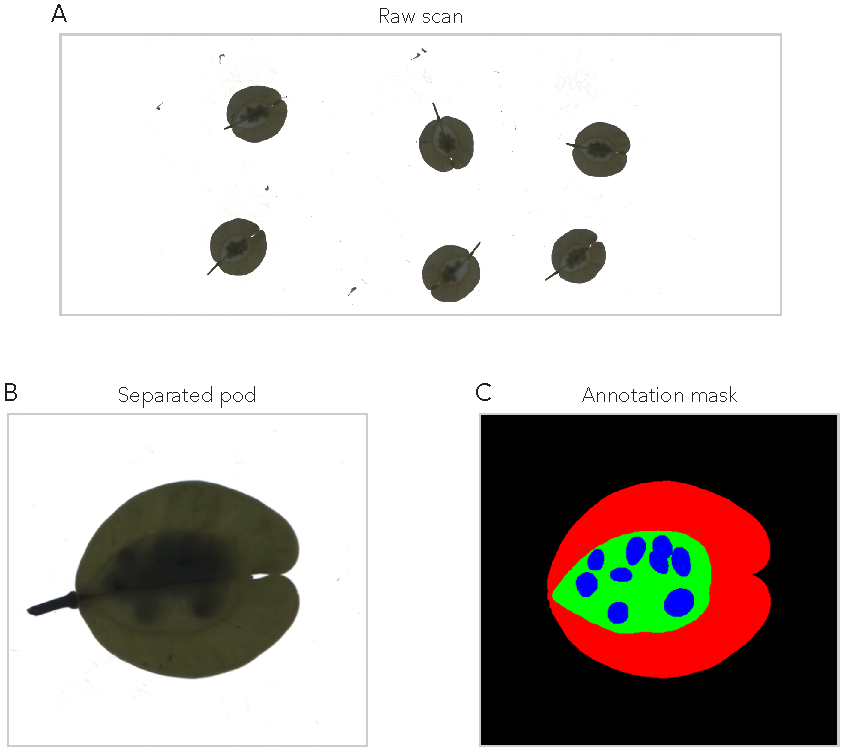
\includegraphics[width=\linewidth]{figures/pennycress-unet/pennycress_scan_annotation.pdf}
 \captionsetup{justification=raggedright,singlelinecheck=false}
 \caption[Raw pennycress seed-pod scans and pixel-level annotations.]{Raw pennycress seed-pod scan, separated pod crop, and pixel-level annotation. (A) Flatbed scan excerpt showing multiple \textit{Thlaspi arvense} seed pods on a white scanner background before object separation, annotation, and segmentation preprocessing. (B) Separated \textit{T. arvense} seed pod extracted from a raw scan. (C) Corresponding semantic annotation mask, with wing tissue in red, envelope tissue in green, seeds in blue, and background in black.}
 \label{fig:ch2-pennycress-scan-annotation}
\end{figure}

\subsubsection{Data Preprocessing}\label{sec:ch2-preprocessing}
Before model input, we separated each pennycress seed pod in the raw image. We created rectangular bounding boxes around each seed pod object in Python, and we saved each bounding box as a separate image, yielding a dataset of 12,253 individual pods across the 768 scans. We used these separated images for model input.

\subsubsection{Image Tile Generation}\label{sec:ch2-tile-gen}
We implemented a tile generation scheme to increase the amount of training data available and build an invariance to common imperfections that occur during the image collection process. Tiling is a form of image augmentation that divides each image into small, fixed-size patches that serve as training examples.

Prior to tiling, we padded each separated image with 128 pixels in all directions. Image padding enables us to generate tiles near the edge of images, allowing the model to see a greater context. The red box in the leftmost image in Figure~\ref{fig:ch2-pennycress-preproc} highlights the padding boundary, and the remaining panels show the corresponding semantic and class-specific masks used during tile sampling. While we also used a tile size of 128 pixels, the padding and tile size are independent parameters.

After padding, we selected a tile size of 128 pixels. Pixels on the seed pod were randomly initialized as tile centers. After the algorithm selected center pixels, it used the surrounding 128 $\times$ 128 pixels to create each tile.

\begin{figure}[!ht]
 \centering
 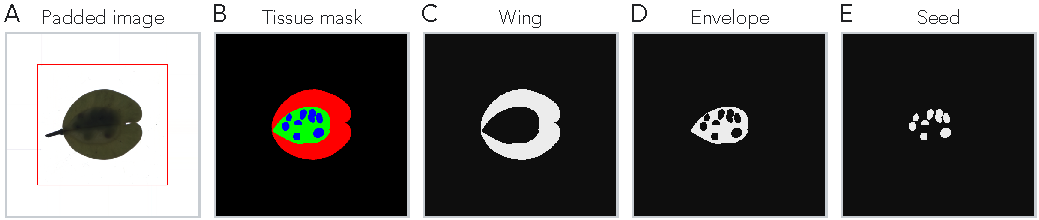
\includegraphics[width=\linewidth]{figures/pennycress-unet/pennycress_preprocessed_images.pdf}
 \captionsetup{justification=raggedright,singlelinecheck=false}
 \caption[Preprocessing outputs for model training.]{Preprocessing outputs for model training. (A) Padded separated pod image; the red rectangle marks the original crop boundary after adding 128 pixels of context on each side. (B) Full semantic tissue mask. (C--E) Binary masks for wing, envelope, and seed classes, respectively.}\label{fig:ch2-pennycress-preproc}
\end{figure}

During validation, we left tiles unchanged to prompt the most accurate predictions possible. However, during training, we applied various image augmentations and transformations to build an invariance to common data collection issues. We applied rotation, blur, saturation, brightness, flips, and transposes with a 50\% chance of occurrence each, greatly increasing the number of unique types of tiles that could be generated.

We selected each type of transformation to combat certain issues that occur during the scanning process. For example, blur transformations simulate potential smudges on the scanner screen. Rotations model the differences in angle between scanned seed pods, and brightness transformations capture the potential for shadows underneath folds in an image. By using these transformations to simulate real imaging issues, the model learns to become invariant to such features and instead focus on biologically relevant information. Therefore, the tile generation scheme serves two purposes. It increases the amount of available training data, and it builds an invariance to common scanning issues. We show examples of generated training tiles, their corresponding labels, and representative augmentation outputs in Figure~\ref{fig:ch2-tile-gen-ex}.

\begin{figure}[!ht]
 \centering
 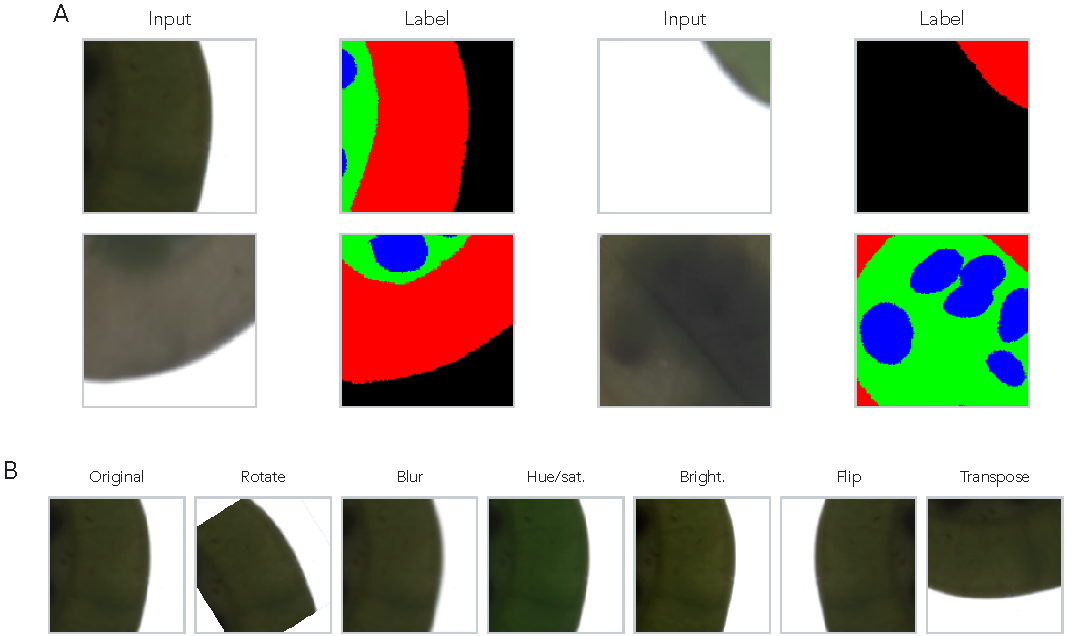
\includegraphics[width=\linewidth]{figures/pennycress-unet/tile_gen.pdf}
 \captionsetup{justification=raggedright,singlelinecheck=false}
 \caption[Example training tiles and augmentation outputs.]{Example training tiles and augmentation outputs. (A) Input and label pairs show 128$\times$128 tiles sampled from padded seed-pod images and their corresponding tissue-label masks. Tiles include background, pod-boundary, tissue, and seed contexts used for model training. (B) Representative image-tile augmentations show the transformation families applied during training, including affine rotation, blur, hue/saturation shift, brightness/contrast adjustment, flip, and transpose operations.}\label{fig:ch2-tile-gen-ex}
\end{figure}

\subsection{U-Net Baseline}\label{sec:ch2-unet}
\subsubsection{Architecture}
We used U-Net \cite{unet}, a fully convolutional encoder-decoder architecture in which a contractive path captures hierarchical context and a symmetric, expansive path recovers spatial localization. We adapted the original architecture with a modified block structure, SELU activations, and tuned hyperparameters for tissue-level pod segmentation.

Because raw seed pod images were too large and computationally expensive to fit into model memory while training, we used the generated tiles created in Section~\ref{sec:ch2-tile-gen} for training.

The model's input is a 3-channel RGB tile of size 128 $\times$ 128, and its output is also 128 $\times$ 128 with four channels corresponding to background, wing, envelope, and seed classes. We applied a softmax activation function to create a pixel-wise segmentation map, where the model gives each pixel a class label. We then compared segmentation maps to the corresponding hand-annotated segmentations detailed in Section~\ref{sec:ch2-annotation} and minimized the weighted cross-entropy loss between them to train the model.

The main component in the U-Net architecture is a convolutional block. Each block contains three convolutional layers with 3 $\times$ 3 kernels; each convolution is followed by batch normalization, SELU activation, and dropout with a rate of 0.1.

The network comprises nine convolutional blocks (Figure~\ref{fig:ch2-pennycressunet}), beginning with a 32-kernel block at the full 128$\times$128 tile resolution. The four contractive blocks are separated by 2$\times$2 max-pooling that halves spatial resolution while increasing the channel depth from 32 to 256. A 512-kernel bottleneck operates at 8$\times$8 resolution. The four expansive blocks reverse this with upsampling-convolution steps that restore spatial resolution and reduce channel depth, returning to 128$\times$128. Skip connections concatenate contractive and expansive feature maps, improving gradient flow and fusing features across scales. A final 1$\times$1 convolution produces the four-channel segmentation map.

\begin{figure}[!ht]
 \centering
 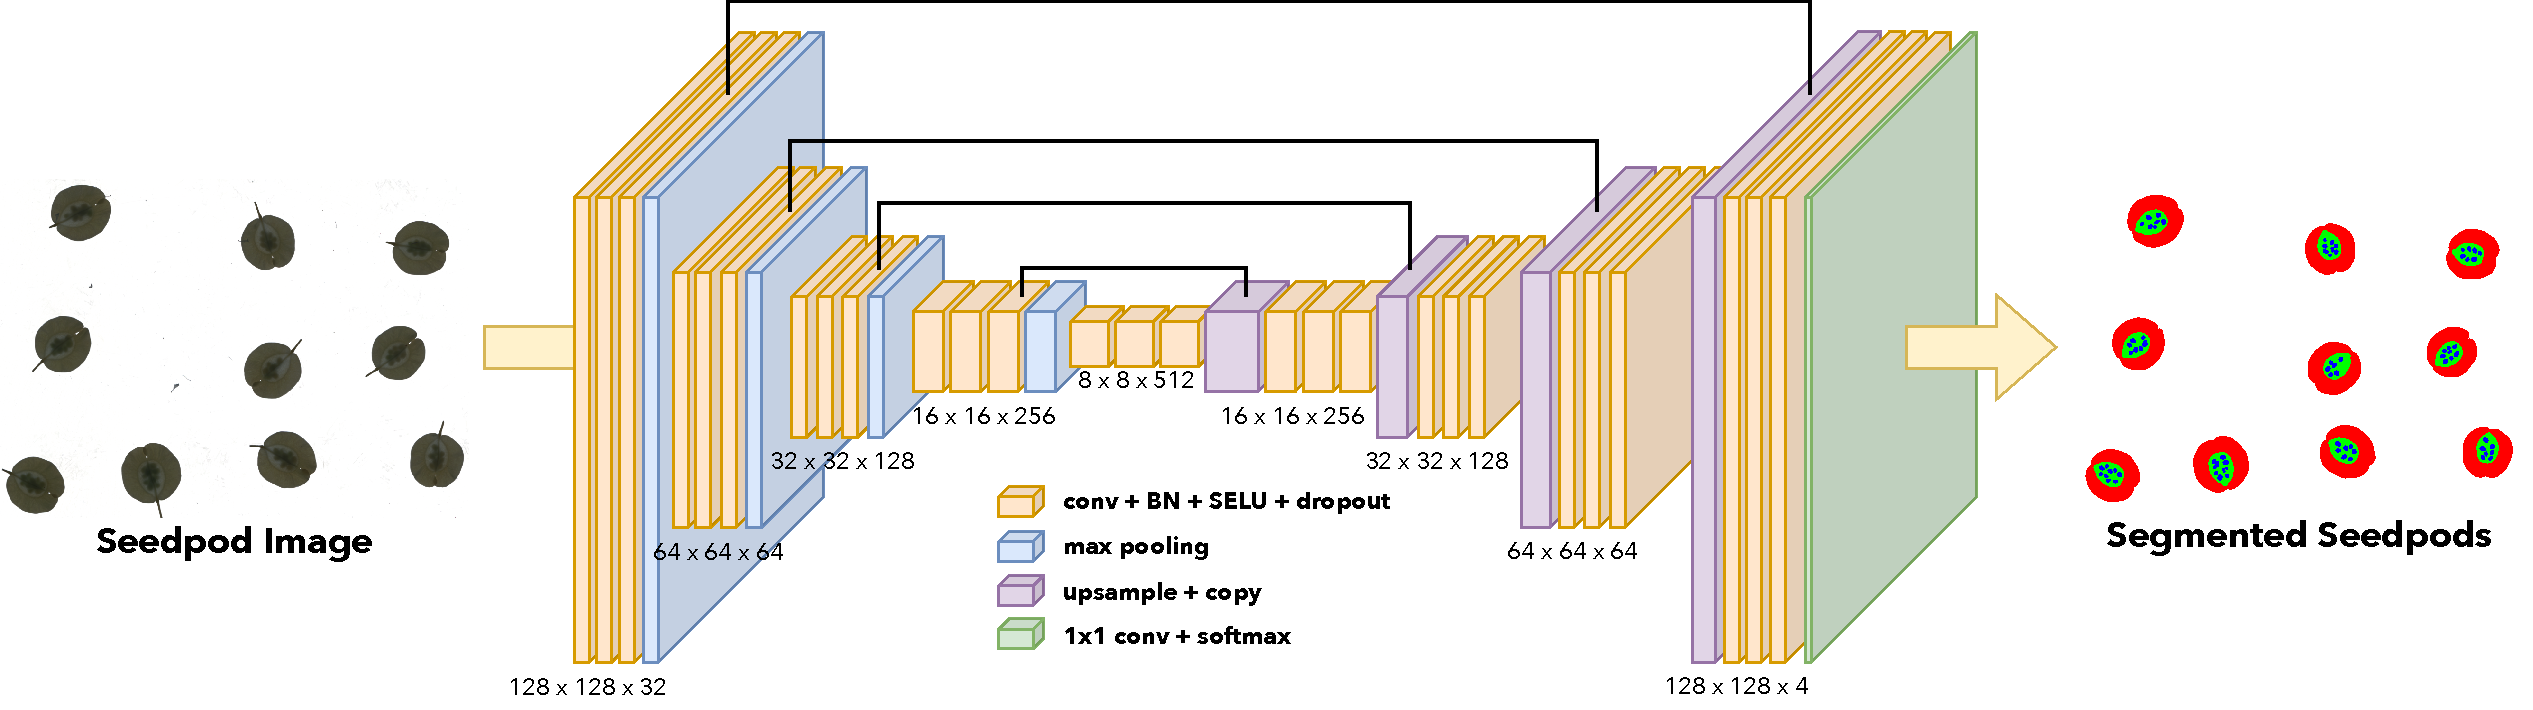
\includegraphics[width=\linewidth]{figures/pennycress-unet/PennycressUNet.pdf}
 \captionsetup{justification=raggedright,singlelinecheck=false}
 \caption[Pennycress U-Net architecture]{Pennycress U-Net architecture. The model takes a 128$\times$128 RGB seed pod tile as input and returns a 128$\times$128 four-channel semantic segmentation map for background, wing, envelope, and seed classes. Orange blocks denote 3$\times$3 convolution, batch normalization (BN), SELU activation, and dropout; blue blocks denote max pooling; purple blocks denote upsampling with skip-copy connections; and the green block denotes the final 1$\times$1 convolution with softmax output. Feature-map labels are shown as height $\times$ width $\times$ channels.}
 \label{fig:ch2-pennycressunet}
\end{figure}

\subsubsection{Boundary-Weighted Cross Entropy Loss}
To account for uncertainty in the exact boundaries of our ground-truth labels, we implemented a weighted cross-entropy loss that scales the per-pixel loss by a boundary-aware weight map.

We first compute a raw weight map from the eroded seed mask. We binarize the seed channel, subtract its binary erosion to isolate the boundary ring, and then calculate the Euclidean distance from each pixel to the closest border pixel to produce a distance map. We clip distances at a maximum of $b = 5$ pixels and normalize to the range $[0, 1]$. We evaluated two configurations parameterized by a border weight $w_b$.

In the \textbf{boundary down-weighted} configuration ($w_b < 1$), we min-max normalize the raw weight map so that pixel values $W_{i,j} \in [0, 1]$, where $i$ and $j$ index the row and column of a pixel within a tile. We then invert the weight map so that pixels with a smaller distance to the boundary have a lower weight value. Finally, we scale the weight map so that its range is $W_{i,j} \in [w_b, 1]$. This configuration treats boundary annotations as the noisiest signal and lets the model rely more on confidently-labeled interior pixels.

In the \textbf{boundary up-weighted} configuration ($w_b > 1$), we instead clip the raw weight at a minimum of $1$, yielding $W_{i,j} \in [1, w_b]$ so that distant pixels carry weight $1$ and boundary pixels carry weight up to $w_b$. This configuration treats boundaries as the most informative regions to learn.

We then multiply the weight map pixelwise with cross-entropy loss and average over pixels:

\begin{align}\label{eq:ch2-wce}
 L_{WCE}(t, p(\theta)) = - \frac{1}{\mid I \mid \mid J\mid} \sum_{j}^{J} \sum_{i}^{I} \sum_{k}^{K} W_{i,j} (t_{i,j,k} \log(p(\theta)_{i,j,k})),
\end{align}

\noindent where $t$ is the ground truth segmentation map and $p(\theta)$ is the predicted segmentation map as a function of U-Net parameters. The indices $i$ and $j$ run over the $I$ rows and $J$ columns of a tile, so $\mid I \mid \mid J \mid$ is the number of pixels the loss is averaged over, and $k$ runs over the $K = 4$ classes (background, wing, envelope, and seed). For a given pixel, $t_{i,j,k}$ is $1$ if that pixel is labeled class $k$ in the ground truth and $0$ otherwise, while $p(\theta)_{i,j,k}$ is the softmax probability the model assigns to class $k$ at that pixel. The inner sum over $k$ therefore reduces to the log-probability the model placed on the correct class, and $W_{i,j}$ rescales that pixel's contribution according to its distance from a seed boundary.

\subsubsection{Model Training}
We trained the U-Net for up to 150,000 mini-batch updates using the Adam optimizer with a batch size of 32. Rather than partitioning training into fixed epochs over the tile dataset, we sampled tiles continuously from the train split (Section~\ref{sec:ch2-pennycress-dataset}) and tracked progress by iteration count. We evaluated validation loss every 1,000 batches and applied an early stopping criterion of 50 evaluation intervals. If the best validation loss did not improve over 50 consecutive checkpoints (50,000 batches), training terminated.

We used a learning rate schedule with linear warmup and cosine decay. The learning rate ramped from 0 to $1\!\times\!10^{-3}$ over the first 1,000 batches to stabilize early gradients, then decayed via a cosine schedule to $1\!\times\!10^{-5}$ over the subsequent 90,000 iterations and held constant thereafter.

\subsection{Phenotype Extraction}\label{sec:ch2-phenotype-extraction}

We developed functions to extract 52 features from each seed pod segmentation map, grouped into three categories: absolute, ratio, or color.

\subsubsection{Absolute Features}

We calculated seven absolute features from each segmentation map: wing area and perimeter, envelope area and perimeter, seed area and perimeter, and seed count. Areas for each tissue were calculated by summing the pixels assigned to that class. Perimeters were calculated using Scikit-Image~\cite{scikit-image} on nested binary masks. Wing perimeter was calculated from the union of wing, envelope, and seed pixels, envelope perimeter was calculated from the union of envelope and seed pixels, and seed perimeter was calculated on the raw (pre-watershed) seed mask, giving the total boundary length of all seed pixels in the pod. Pixel counts were converted to physical area by dividing by DPI$^2$ ($600^2=360,000$) and multiplying by 6.4516 cm$^2$/in$^2$.

In addition to measuring area and perimeter features, we utilized the watershed algorithm to count the number of seeds in each segmented image. First, we isolated the seed channel and applied a morphological opening to suppress noise. Then, we calculated the Euclidean distance from each seed pixel to the nearest non-seed pixel. We applied a threshold to this distance map, setting any pixel that was less than 60\% of the maximum distance value in the map to 0. The thresholded foreground was labeled into connected components and passed as markers to the OpenCV~\cite{opencv_library} watershed algorithm, which returned a per-seed segmentation; seed count is defined as the number of unique markers in the map. The watershed process is visualized in Figure~\ref{fig:ch2-watershedding}.

\begin{figure}[!ht]
 \centering
 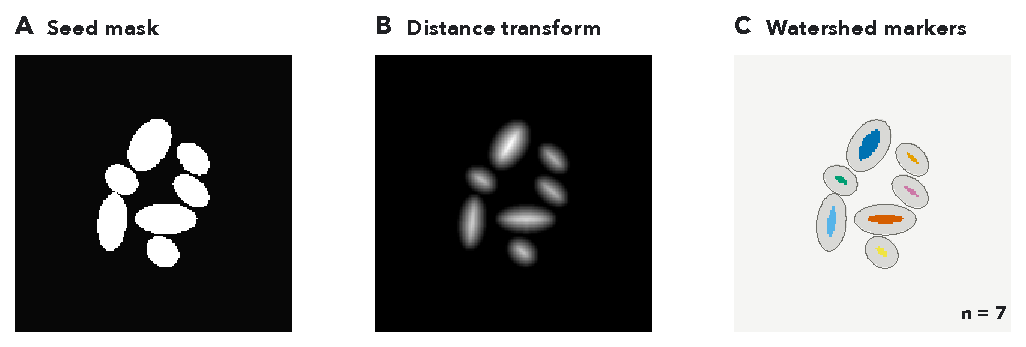
\includegraphics[width=\linewidth]{figures/pennycress-unet/watershedding.pdf}
 \captionsetup{justification=raggedright,singlelinecheck=false}
 \caption[Seed-count extraction by watershed segmentation]{Seed-count extraction by watershed segmentation. (A) Binary seed mask isolated from the U-Net segmentation map. (B) Euclidean distance transform used to identify seed interiors. (C) Connected-component markers after thresholding the distance map at 60\% of its maximum value; colors denote marker identities used to initialize watershed segmentation, and the resulting marker count defines seed count.}
 \label{fig:ch2-watershedding}
\end{figure}

\subsubsection{Ratio Features}
We calculated 18 ratio features from the segmented seed pod masks, with six to-total ratios and twelve between-tissue ratios, evenly split between area and perimeter-based variants. The six to-total ratios divide each tissue's area or perimeter by the total area or perimeter, yielding wing-to-total, envelope-to-total, and seed-to-total ratios for both measurement types.

The 12 between-tissue ratios cover all pairs of distinct tissues for both area and perimeter. These include ratios into seed (envelope/seed, wing/seed), into envelope (wing/envelope, seed/envelope), and into wing (seed/wing, envelope/wing), computed for both measurement types. Reciprocal ratios are retained (e.g., seed/envelope and envelope/seed) so that downstream analysis is not restricted.

\subsubsection{Color Features}
We extracted nine color features from each tissue: red, green, blue (RGB); hue, saturation, brightness (HSV); and lightness, $a^*$ (green-red), and $b^*$ (blue-yellow) from CIELAB. We converted each input image into all three color spaces using OpenCV~\cite{opencv_library}. We then created a tensor of these features with size $\texttt{height} \times \texttt{width} \times 9$. We used the segmentation masks to subset this tensor by tissue, yielding three sub-tensors covering wing, envelope, and seed features separately.

We aggregated each color channel across spatial dimensions by taking the mean over the relevant tissue's pixels, producing a nine-dimensional color vector per tissue. Across the three tissues, this yielded 27 features in total.

\subsection{Segmentation Architecture Benchmarking}\label{sec:ch2-benchmark}
To ensure that our pipeline extracts the most accurate downstream phenotypes possible, we identified the most effective segmentation architecture. We tested six architectures across three families: CNNs, transformers, and foundation models.

We compared two CNN architectures to the baseline U-Net: nnU-Net \cite{isensee2021nnu} and DeepLabV3+ \cite{chen2018encoder}. nnU-Net is an approach that configures a U-Net systematically through a three-stage pipeline. The selection process includes fixed parameters that generalize across many datasets; rule-based parameters that are determined by unique dataset and pipeline characteristics; and empirical parameters that are learned through trial and error. Because nnU-Net derives its own patching, batch size, and augmentation scheme through fingerprinting and rule-based selection, the benchmarking for this architecture did not include our custom tile generation scheme (Section~\ref{sec:ch2-tile-gen}). DeepLabV3+ combines an encoder-decoder architecture with atrous depthwise separable convolutions, balancing the use of long-range spatial context with fine-grained boundary detection.

We selected SegFormer \cite{xie2021segformer} and Mask2Former \cite{cheng2022masked} as exemplar transformer architectures for benchmarking. SegFormer uses a hierarchical transformer encoder backbone that generates both high-resolution, fine-grained features and low-resolution, coarse features, and a lightweight MLP decoder to fuse these features for the final semantic segmentation task. Unlike SegFormer, which optimizes a per-pixel classification objective, Mask2Former adopts an alternate paradigm based on set prediction. Mask2Former uses a multi-scale encoder backbone to extract features, which are then upsampled to high-resolution per-pixel embeddings with a pixel decoder. Additionally, Mask2Former utilizes a transformer decoder with learnable query inputs to predict mask candidates. These queries are refined through cross-attention with the multi-scale features, and the transformer decoder output and pixel decoder output are combined via dot product to produce region predictions. Although Mask2Former is designed to be a general segmentation architecture, supporting panoptic, instance, and semantic segmentation, we trained only for a semantic segmentation objective due to our task formulation.

We evaluated SAM 3 \cite{carion2025sam3} as a candidate foundation model for benchmarking. SAM 3 is a foundation model designed for promptable concept segmentation, taking input as either text or image exemplars. SAM 3 was trained with a model-in-the-loop data engine on over 1 billion images, generating segmentation examples using human input while shifting towards more model reliance during the annotation process. Although SAM 3 is capable of segmenting video and using concept prompts, we focused on the benefits that its pretrained encoder provides, adopting an approach similar to ClassWise-SAM-Adapter \cite{pu2025classwise} by using a lightweight convolutional mask decoder for classwise semantic segmentation. Furthermore, we applied Low-Rank Adaptation (LoRA) \cite{hu2022lora} to the image encoder to enable parameter-efficient fine-tuning and limit drift from pretrained representations.

We trained DeepLabV3+, SegFormer, and Mask2Former from default pretrained backbones with the same tile generation and preprocessing scheme that we used for our custom U-Net to ensure consistency. Since nnU-Net's data-aware preprocessing approach is emphasized as one of its strengths, we did not apply our custom preprocessing pipeline to it, instead using nnU-Net's adaptive fingerprinting setup for preprocessing and model training. As a consequence, nnU-Net scored predictions under its own pipeline at the level of individual seed pod crops (65 crops), whereas all other architectures were evaluated on the five full images from the same test split. For comparability, we grouped nnU-Net crop-level predictions by their source full image before computing the per-image metrics reported below.

For all models except nnU-Net and Mask2Former, we trained variants with unweighted, up-weighted, and down-weighted boundary loss. Due to nnU-Net's adaptive pipeline and Mask2Former's mask-classification objective, boundary weighting was not compatible with these architectures. These model families provide coverage across architectures (CNN and transformer), training objectives (per-pixel prediction and set prediction), and learning scenarios (supervised pretraining and foundation model pretraining).

We used intersection over union (IoU), also known as the Jaccard index, as the primary evaluation metric for this project, following its established use as the standard measure for semantic segmentation benchmarks \cite{everingham2010pascal}. Given a ground truth pixel-wise segmentation set \textit{A} and a predicted pixel-wise segmentation set \textit{B} for a single class on a single image, the IoU is defined as:
\begin{align}\label{eq:ch2-iou}
 \mathrm{IoU}(A,B) &= \frac{|A \cap B|}{|A \cup B|}.
\end{align}

IoU lies in $[0, 1]$, with a value of $1$ indicating identical sets and $0$ indicating disjoint sets. We report class-wise IoU for each tissue class (wing, envelope, seed), reflecting the differing biological importance and segmentation difficulty of each class. We additionally report the mean IoU (mIoU) as a single-number summary used to rank models during benchmarking. We compute IoU separately for each test image and summarize it as a mean and standard deviation across images, rather than pooling pixels over the whole test set, because per-image scores are more informative than a single dataset-level score for segmentation evaluation \cite{csurka2013evaluation}. For consistency, we compute IoU identically across all architectures.

\subsection{Predictive Phenotype Networks}\label{sec:ch2-pen}
To explore the relationships between measured phenotypes, we produced predictive phenotype networks (PPNs) using iRF-LOOP \cite{cliff2019high}. Given an input set of extracted phenotypes for each pod, we computed the average value for each accession, which we used as input to the model. iRF-LOOP uses iterative random forest \cite{basu2018iterative} to predict a single held out phenotype from all others. Iterative random forest modifies the probability that each feature is sampled to create splits in the decision trees, weighting it by the feature's importance in the previous iteration. Because all iRF-LOOP tasks in our phenotype set are regression tasks, importance is measured by Mean Decrease in Impurity (MDI), which captures the normalized total reduction in mean squared error attributable to each feature across all trees, normalized to sum to one. Using this process, informative features are selected more frequently as the model converges. This process is repeated by holding out each phenotype, with the entire model output yielding pairwise importance values between phenotypes.

Using the iRF-LOOP output, we constructed PPNs, which take the form of a directed graph, where nodes represent phenotypes and edges represent predictive relationships. An edge from phenotype A to phenotype B indicates that A is predictive of B, with edge weight equal to the iRF-LOOP importance of A in predicting B. Using the raw iRF-LOOP output produced a dense network with all phenotypes connected to all others; however, we induced sparsity and highlighted only strong predictive relationships by retaining only edges whose weight falls in the top 5\%. For interpretation, we also visualized the subset of retained edges that connect traits measured from different pod tissues. PPN outputs allowed us to perform an exploratory analysis of relationships between phenotypes before downstream analysis.

\subsection{Genome-Wide Association Study}\label{sec:ch2-gwas}
After measuring seed pod phenotypes and their relationships on a population scale, we performed a GWAS to find significant associations between SNP loci and variation in phenotypic traits.

\subsubsection{Phenotype Curation and Heritability Estimation}\label{sec:ch2-heritability}
Before running association tests, we assessed whether each phenotype had sufficient genetic signal to warrant GWAS by estimating broad-sense heritability in the dryland environment, in which the pod-morphology phenotypes analyzed here were measured. Because most accessions in our panel are unreplicated, $H^2$ was estimated on the subset of $n=25$ replicated genotypes. For each phenotype, we fit a linear mixed model with genotype as a random effect and computed
\[
H^2 = \sigma^2_G / (\sigma^2_G + \sigma^2_E),
\]
where $\sigma^2_G$ and $\sigma^2_E$ are genotypic and residual variance components. Phenotypes with $H^2 < 0.05$ were removed from downstream association analyses due to lacking sufficient heritable signal. We additionally restricted our analysis to phenotypes derived from the U-Net segmentation pipeline described in Section~\ref{sec:ch2-unet}, excluding manually measured traits to maintain methodological consistency. Per-trait $H^2$ for the screened traits is reported in Table~\ref{tab:ch2-heritability}.

\begin{table}[p]
 \centering
 \caption[Broad-sense heritability of the 34 U-Net derived pod traits]{Broad-sense heritability ($H^2$) of the 34 U-Net-derived pod traits in the dryland environment that passed the $H^2 \geq 0.05$ screen and were carried into GWAS. $H^2$ was estimated from a linear mixed model with genotype as a random effect, fit on 25 replicated genotypes (2--3 replicate images per genotype; $\sim$15 pods per replicate image). Significance $p$ is from a restricted likelihood-ratio test on the genotype variance component ($H_0\!:\sigma^2_G = 0$). Traits marked $\dagger$ yielded significant GWAS associations (Table~\ref{tab:ch2-gwas-results}); note that heritability was necessary but not sufficient for a GWAS hit.}\label{tab:ch2-heritability}
 \footnotesize
 \setlength{\tabcolsep}{6pt}
 \renewcommand{\arraystretch}{1.0}
 \begin{tabularx}{\textwidth}{@{}>{\raggedright\arraybackslash}X c c@{}}
 \toprule
 Trait & $H^2$ & Significance ($p$) \\
 \midrule
 envelope-to-wing area ratio & 0.461 & $<0.0001$ \\
 envelope-to-total area ratio & 0.423 & 0.0002 \\
 wing-to-envelope area ratio & 0.409 & 0.0003 \\
 envelope perimeter & 0.390 & 0.0016 \\
 envelope area & 0.389 & 0.0017 \\
 wing-to-total area ratio & 0.387 & 0.0003 \\
 \textbf{wing area}$^\dagger$ & 0.366 & 0.0010 \\
 wing HSV saturation & 0.321 & 0.0022 \\
 wing perimeter & 0.302 & 0.0060 \\
 seed area & 0.297 & 0.0214 \\
 envelope-to-wing perimeter ratio & 0.292 & 0.0006 \\
 wing-to-envelope perimeter ratio & 0.287 & 0.0009 \\
 \textbf{wing-to-seed area ratio}$^\dagger$ & 0.285 & 0.0077 \\
 seed perimeter & 0.263 & 0.0334 \\
 seed-to-wing area ratio & 0.247 & 0.0117 \\
 envelope-to-total perimeter ratio & 0.230 & 0.0051 \\
 wing CIELAB $b^*$ & 0.227 & 0.0525 \\
 envelope HSV saturation & 0.220 & 0.0418 \\
 seed count & 0.218 & 0.0319 \\
 \textbf{envelope CIELAB $b^*$}$^\dagger$ & 0.217 & 0.0315 \\
 seed RGB red & 0.204 & 0.0881 \\
 \textbf{envelope-to-seed area ratio}$^\dagger$ & 0.200 & 0.0501 \\
 seed CIELAB $b^*$ & 0.190 & 0.0627 \\
 seed-to-envelope area ratio & 0.188 & 0.0681 \\
 seed-to-total area ratio & 0.188 & 0.0453 \\
 seed HSV hue & 0.185 & 0.0796 \\
 seed HSV saturation & 0.155 & 0.1048 \\
 wing RGB blue & 0.131 & 0.1770 \\
 seed HSV brightness & 0.120 & 0.1518 \\
 seed CIELAB lightness & 0.097 & 0.1672 \\
 envelope RGB green & 0.089 & 0.2169 \\
 envelope CIELAB lightness & 0.086 & 0.2213 \\
 seed RGB blue & 0.083 & 0.1234 \\
 envelope HSV brightness & 0.068 & 0.2530 \\
 \bottomrule
 \end{tabularx}
\end{table}

\subsubsection{Genotypic Data}
SNP genotypes were drawn from the imputed, lightly filtered whole-genome resequencing dataset of \textit{Thlaspi arvense} natural accessions generated by Wu et al.\ \cite{wu2025thlaspi}. We applied additional quality-control filtering: SNPs with severe departures from Hardy--Weinberg equilibrium ($p < 1\times10^{-150}$) were removed, genotypes with more than 10\% missing calls were dropped, and the highly differentiated Armenian subpopulation was excluded. The resulting dataset comprised 423 genotypes and $1{,}975{,}204$ SNPs. Association testing was restricted to the 189 accessions with matched U-Net-derived pod phenotypes.

\subsubsection{Association Testing}
We fit four single- and multi-locus association models implemented in GAPIT (Genome Association and Prediction Integrated Tool) \cite{wang2021gapit}: MLM \cite{yu2006mlm}, MLMM \cite{segura2012mlmm}, FarmCPU \cite{liu2016farmcpu}, and BLINK \cite{huang2019blink}. We further restricted the marker set to the $1{,}759{,}624$ SNPs with a minor allele frequency (MAF) $\geq 0.03$. We ran GWAS independently per phenotype and retained the union of SNPs reaching $p < 1\times10^{-6}$ under any of the four models. Because extensive linkage disequilibrium makes the per-SNP tests non-independent, a Bonferroni correction is overly stringent; we therefore treated raw $p < 1\times10^{-6}$ as a suggestive association cutoff and deferred false-positive control to GRIN (Section~\ref{sec:ch2-grin}).

\subsubsection{SNP-to-Gene Assignment}\label{sec:ch2-snp2gene}
After finding significant loci, we mapped SNPs to candidate genes using a two-pronged approach. For each significant SNP, we first fit a local linkage disequilibrium (LD) decay curve and defined a data-driven window around the SNP based on fitted decay distance. We then identified all genes whose coordinates fall within this window on the pennycress TAV2 reference genome. When LD decay could not be reliably fit for a SNP, we instead assigned the two nearest flanking genes (one upstream and one downstream) by physical distance. Because functional annotation of the pennycress genome is limited, we annotated each assigned pennycress gene by its best BLAST-hit Arabidopsis ortholog from TAIR \cite{garcia2002tair} to enable downstream biological interpretation.

\subsubsection{Candidate Gene Set Construction}
We aggregated candidate genes by taking the union of genes mapped from significant SNPs, regardless of which GWAS method produced the original association. We restricted our downstream analysis to traits with considerable heritability ($H^2 \geq 0.05$) and to phenotypes derived from the U-Net segmentation pipeline. Under these restrictions, four pod-related phenotypes (envelope CIELAB $b^*$, envelope-to-seed area ratio, wing area, and wing-to-seed area ratio) yielded significant GWAS hits, mapping to 6 unique SNPs and 69 pennycress genes, 64 of which had annotated Arabidopsis TAIR orthologs. We note that these four phenotypes are highly correlated, as they are geometric ratios computed from a common set of pod measurements. They therefore do not represent four biologically independent signals. These 64 orthologs constitute the candidate ortholog set, which we filtered with GRIN (Section~\ref{sec:ch2-grin}) before \textsc{Mentor} module derivation (Section~\ref{sec:ch2-mentor}).

\subsection{\textsc{Mentor} Module Derivation}\label{sec:ch2-mentor}
\subsubsection{GRIN Filtering}\label{sec:ch2-grin}
Before using our candidate genes as input to \textsc{Mentor} for module construction, we applied GRIN \cite{sullivan2024grin} to reduce potential false-positive genes. Both GRIN and \textsc{Mentor} operate over a nine-layer \textit{Arabidopsis thaliana} multiplex network spanning a pool of 26,605 genes, in which each layer encodes a distinct line of biological evidence: protein--protein interaction, transcriptional regulation from two independent sources, gene co-expression, co-evolution, knockout phenotype similarity, methylation-derived predictive relationships, metabolic pathway membership, and a diversity-derived layer. All nine layers are undirected and unweighted, and each contributes equally to network propagation; per-layer sources and sizes are given in Table~\ref{tbl:multiplex-layers}. Given a candidate gene set, whose members serve as the seed nodes from which network propagation begins, and this multiplex network \cite{kainer2025rwrtoolkit}, GRIN operates in two stages. First, it runs random walk with restart (RWR) from the seed nodes, yielding a rank vector of the genes in the network most closely related to them; in parallel, it runs RWR on 100 randomly sampled gene sets of the same size, creating a null distribution rank vector. Next, GRIN uses a sliding-window Mann-Whitney U test to evaluate the likelihood of observing the seed-node RWR ranks at random. With this sliding window, a threshold can be defined where the ranks become insignificant. The resulting significant genes are retained, while all others are dropped. GRIN retains genes that are more tightly connected in the multiplex network to the rest of the candidate set; this network proximity is taken as a proxy for shared biological function. In this paradigm, GRIN assumes that well-connected genes may jointly contribute to the associated phenotype. We refer to the genes GRIN retains as the network-supported gene set.

\subsubsection{Module Construction}
We applied \textsc{Mentor}, a multi-step framework for deriving functionally related genetic modules, using the multiplex network and the network-supported gene set as input \cite{mentor}. We used the \textit{Arabidopsis thaliana} multiplex because this close relative has richer functional annotation and network resources than pennycress.

Starting from the network-supported gene set (Section~\ref{sec:ch2-grin}), \textsc{Mentor} applies RWR as a diffusion method to measure the probability of traveling to each gene in the multiplex from all genes in that set. Each seed node produces its own score vector over all multiplex nodes, with indices representing the probability of reaching each node from that seed. The score vectors are then rank-ordered, truncated at the elbow of the mean score-versus-rank curve, and converted into a dissimilarity matrix by taking $(1 - \rho)$, with $\rho$ representing Spearman correlation, between each pair of genes' rank-ordered score vectors. With the resulting dissimilarities, \textsc{Mentor} creates a dendrogram using agglomerative clustering with complete linkage as our module distance measure. This dendrogram is then thresholded to examine modules of a certain size.

\subsection{\textsc{Mentor-IA} Interpretation}\label{sec:ch2-mentor-ia}
After deriving a set of modules with \textsc{Mentor}, we used \textsc{Mentor-IA} to explore the biological mechanisms associated with these modules \cite{mentor-ia}. \textsc{Mentor-IA} is a multi-agent LLM framework for mechanistic interpretation, in which specialized agents each contribute to a distinct line of evidence. These agents include a mygene interpreter, which utilizes gene summaries, GO terms, and pathway annotations to explore each gene's role individually; a literature agent, which explores mechanistic connections in related literature via Europe PMC; an enrichment agent, which tests whether a module is enriched for pathways in GO, KEGG, or Reactome; a network agent, which uses subgraph evidence to refine the interpretation; and a meta aggregator, which synthesizes evidence to produce a coherent mechanistic summary.

Using the evidence provided by \textsc{Mentor-IA} as a starting point, we manually examined pennycress and \textit{Brassicaceae} literature to assess whether the proposed mechanisms were consistent with known biology.

\subsection{Statistical Analysis}
This section summarizes the statistical analyses applied at each stage of the pipeline. Models, sample sizes, and significance thresholds are specified in the referenced sections, and the tables cited below report the resulting statistics.

Segmentation accuracy was evaluated with per-class IoU and mIoU (Section~\ref{sec:ch2-benchmark}), computed per test image and summarized as mean $\pm$ standard deviation in Table~\ref{tab:ch2-pennycress-results}. We additionally profiled the computational efficiency of each benchmarked architecture---parameter count, mean per-image inference time, and peak allocated GPU memory on the test set---reported in Table~\ref{tab:ch2-efficiency} and Figure~\ref{fig:ch2-accuracy-efficiency}.

Predictive phenotype networks were constructed with iRF-LOOP, using Mean Decrease in Impurity as the edge-weight statistic (Section~\ref{sec:ch2-pen}). Broad-sense heritability was estimated from a linear mixed model with genotype as a random effect (Section~\ref{sec:ch2-heritability}); per-trait $H^2$ and the significance of the genotype variance component are reported in Table~\ref{tab:ch2-heritability}. Association testing used four models implemented in GAPIT (Section~\ref{sec:ch2-gwas}); retained associations, lead SNPs, and their unadjusted $p$-values are reported in Table~\ref{tab:ch2-gwas-results}. Candidate genes were then filtered on network connectivity using the sliding-window Mann-Whitney U test implemented in GRIN (Section~\ref{sec:ch2-grin}).

\section{Results}
We present our results in two stages: the first converts raw pod scans into a per-accession trait matrix, and the second carries that matrix toward candidate genetic mechanisms. In the first stage, we benchmarked segmentation architectures and selected U-Net, extracted per-pod phenotypes from the predicted masks, and applied the trained model at population scale to assemble the trait matrix. We then examined the trait matrix for biological coherence using a predictive phenotype network; this analysis is exploratory and validates the extracted phenotypes rather than selecting which traits enter the downstream analysis. In the second stage, we filtered the trait matrix by heritability, combined the retained traits with genome-wide resequencing genotypes for GWAS, and mapped the associated SNPs to candidate genes. We then pruned those candidates with GRIN, resolved the survivors into modules with \textsc{Mentor}, interpreted the modules with the assistance of \textsc{Mentor-IA}, and assessed whether the prioritized candidates are expressed in pod tissue.

\subsection{Segmentation Benchmark}
\begin{table}[htbp]
 \centering
 \caption[Segmentation benchmark results]{Segmentation benchmark results. Per-class IoU (wing, envelope, seed) and mean IoU (mIoU), reported as mean $\pm$ standard deviation (\%) across the five full test images; mIoU is the mean of the three tissue-class IoUs. Standard deviations are population values ($\mathrm{ddof}=0$) computed over the five test images; nnU-Net was scored on pod crops under its own adaptive pipeline (Section~\ref{sec:ch2-benchmark}) and grouped back to the source full images before summary. Bold values denote the best mean score in each column.}\label{tab:ch2-pennycress-results}
 \small
 \setlength{\tabcolsep}{3.5pt}
 \renewcommand{\arraystretch}{1.1}
 \begin{tabular}{@{}lcccc@{}}
 \toprule
 Model & Wing & Envelope & Seed & mIoU \\
 \midrule
 U-Net & 95.60 $\pm$ 0.98 & 82.84 $\pm$ 2.31 & 78.14 $\pm$ 3.83 & 85.53 $\pm$ 1.45 \\
 U-Net-Down & 95.53 $\pm$ 0.92 & \textbf{82.94} $\pm$ 2.35 & \textbf{78.28} $\pm$ 3.59 & \textbf{85.58} $\pm$ 1.46 \\
 U-Net-Up & 95.58 $\pm$ 0.95 & 82.24 $\pm$ 1.79 & 77.60 $\pm$ 3.81 & 85.14 $\pm$ 1.22 \\
 nnU-Net & \textbf{95.77} $\pm$ 0.93 & 81.78 $\pm$ 1.44 & 75.40 $\pm$ 4.65 & 84.32 $\pm$ 1.39 \\
 DeepLabV3+ & 95.19 $\pm$ 0.90 & 81.53 $\pm$ 2.80 & 75.80 $\pm$ 3.93 & 84.17 $\pm$ 1.72 \\
 DeepLabV3+-Up & 95.28 $\pm$ 0.92 & 81.70 $\pm$ 2.72 & 75.64 $\pm$ 3.76 & 84.21 $\pm$ 1.64 \\
 DeepLabV3+-Down & 95.14 $\pm$ 0.91 & 81.31 $\pm$ 2.69 & 75.89 $\pm$ 3.79 & 84.11 $\pm$ 1.52 \\
 SegFormer & 95.03 $\pm$ 0.99 & 80.45 $\pm$ 2.24 & 75.07 $\pm$ 3.95 & 83.52 $\pm$ 1.24 \\
 SegFormer-Up & 94.99 $\pm$ 0.99 & 80.22 $\pm$ 2.18 & 75.23 $\pm$ 4.07 & 83.48 $\pm$ 1.23 \\
 SegFormer-Down & 95.31 $\pm$ 1.04 & 81.68 $\pm$ 2.13 & 76.36 $\pm$ 4.29 & 84.45 $\pm$ 1.15 \\
 Mask2Former & 95.65 $\pm$ 1.15 & 82.80 $\pm$ 3.67 & 76.65 $\pm$ 4.41 & 85.03 $\pm$ 2.05 \\
 SAM 3 & 95.15 $\pm$ 1.54 & 76.42 $\pm$ 4.30 & 65.62 $\pm$ 9.19 & 79.07 $\pm$ 4.04 \\
 SAM 3-Up & 95.35 $\pm$ 1.54 & 76.78 $\pm$ 4.06 & 68.15 $\pm$ 7.33 & 80.09 $\pm$ 3.10 \\
 SAM 3-Down & 94.95 $\pm$ 1.82 & 73.49 $\pm$ 3.92 & 57.61 $\pm$ 9.39 & 75.35 $\pm$ 3.32 \\
 \bottomrule
 \end{tabular}
\end{table}

\begin{table}[htbp]
 \centering
 \caption[Computational efficiency of benchmarked segmentation architectures]{Computational efficiency of the benchmarked segmentation architectures. Parameter count (millions), mean inference time per full test image ($n=5$, ROCm), and peak allocated GPU memory are summarized once per architecture. For architectures with boundary-weighting variants, inference time is averaged across the measured variants because parameter counts and peak allocated memory are architecture-level quantities. For nnU-Net, inference time and peak memory were computed by grouping its pod-crop predictions back to their five source full images. SAM~3 is adapted with LoRA, so only 5.70~M of its parameters are trainable. Bold values denote the lowest cost in each column.}\label{tab:ch2-efficiency}
 \small
 \setlength{\tabcolsep}{6pt}
 \renewcommand{\arraystretch}{1.1}
 \begin{tabular}{@{}lccc@{}}
 \toprule
 Model & Params (M) & Inference time (s/image) & Peak memory (GB) \\
 \midrule
 U-Net & \textbf{12.57} & \textbf{43.1} & \textbf{0.06} \\
 nnU-Net & 65.21 & 202.2 & 0.65 \\
 DeepLabV3+ & 45.67 & 122.7 & 0.18 \\
 SegFormer & 81.97 & 412.1 & 0.39 \\
 Mask2Former & 215.45 & 377.0 & 0.90 \\
 SAM 3 & 459.74 & 400.7 & 1.81 \\
 \bottomrule
 \end{tabular}
\end{table}

\begin{figure}[htbp]
 \centering
 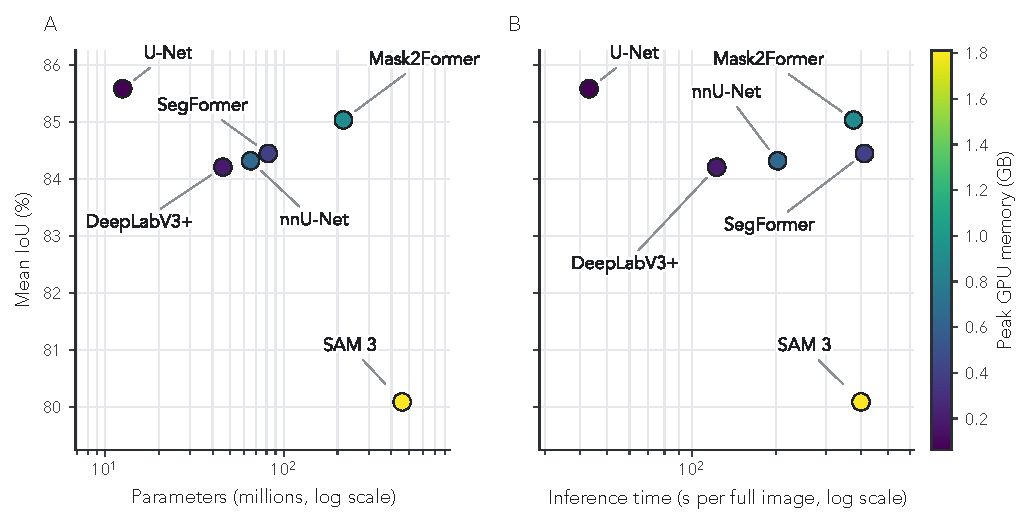
\includegraphics[width=\linewidth]{figures/pennycress-unet/accuracy-efficiency-panels.pdf}
 \captionsetup{justification=raggedright,singlelinecheck=false}
 \caption[Accuracy and computational efficiency of benchmarked segmentation architectures]{Accuracy and computational efficiency of benchmarked segmentation architectures. (A) Best mean IoU (mIoU) achieved by each architecture across its boundary-weighting variants plotted against total parameter count on a log scale. (B) Best mIoU plotted against mean full-image inference time on a log scale, where lower values indicate faster segmentation. Point color and the shared color bar encode peak allocated GPU memory during full-image inference; nnU-Net values were grouped from pod-crop predictions back to the source full images.}
 \label{fig:ch2-accuracy-efficiency}
\end{figure}

We evaluated our models' segmentation performance on 5 raw images containing 65 seed pods in total. Per-class IoU and across-class mIoU are reported in Table~\ref{tab:ch2-pennycress-results}. The boundary down-weighted U-Net achieved the highest mIoU at 85.58\%, narrowly ahead of the baseline U-Net at 85.53\% and Mask2Former at 85.03\%. These top scores were close relative to per-image variation, so we interpret the leading architectures as comparable in accuracy rather than as statistically separable. SAM~3 was the clearest laggard, especially for seed segmentation, where IoU fell as low as 57.61\%.

Efficiency separated the leading architectures more strongly than accuracy (Table~\ref{tab:ch2-efficiency}; Figure~\ref{fig:ch2-accuracy-efficiency}). U-Net used 12.57 million parameters, required 43.1 s per full test image, and peaked at 0.06 GB allocated GPU memory. nnU-Net, DeepLabV3+, SegFormer, Mask2Former, and SAM~3 required more parameters and longer inference times; Mask2Former had a similar mIoU but used 215.45 million parameters, required 377.0 s per full test image, and peaked at 0.90 GB allocated GPU memory. Thus, U-Net provided the most favorable accuracy-efficiency tradeoff for population-scale phenotyping in this small, specialized pod-segmentation task. We found no prior work measuring semantic segmentation of pennycress to compare with our model benchmark suite.

\subsection{Population-Scale Phenotyping}

Having selected U-Net as the most favorable benchmark on accuracy and efficiency, we applied it at population scale to characterize phenotypic structure across the pennycress accession panel. We measured phenotypes from 12,253 seed pods across 768 accessions. Each image yielded approximately 16 retained pod crops on average and took around 2 minutes of model inference time to segment, compared to approximately 1.5 hours of hand segmentation per image, yielding an estimated 30- to 45-fold throughput gain depending on annotator pace.

We used the feature extraction pipeline described in Section~\ref{sec:ch2-phenotype-extraction} to construct an open-source dataset of over 50 phenotypes for all 12,253 seed pods. For visualization and correlation summaries, we excluded detections for which the watershed step returned zero seeds. Figure~\ref{fig:ch2-area-dist} shows the distributions of three key phenotypes: wing area, envelope area, and seed area. These traits correspond directly to the three annotated tissue classes, making their distributions a useful biological plausibility check on segmentation output. Each trait was right-skewed and heavy-tailed, consistent with the log-normal-like distributions commonly observed in quantitative plant traits~\cite{TRY}.

Consistent with the wing-seed regulatory association described in Section~\ref{sec:ch2-pc-background}, wing area was positively correlated with seed area and seed count (Pearson $r = 0.51$ and $0.30$, respectively; Figure~\ref{fig:ch2-wing-seed-corr}). The resulting per-accession phenotype matrix served two roles: as input to iRF-LOOP for PPN construction (Section~\ref{sec:ch2-pen}), and as the candidate trait pool for heritability filtering and GWAS (Section~\ref{sec:ch2-gwas}).

\begin{figure}[!ht]
 \centering
 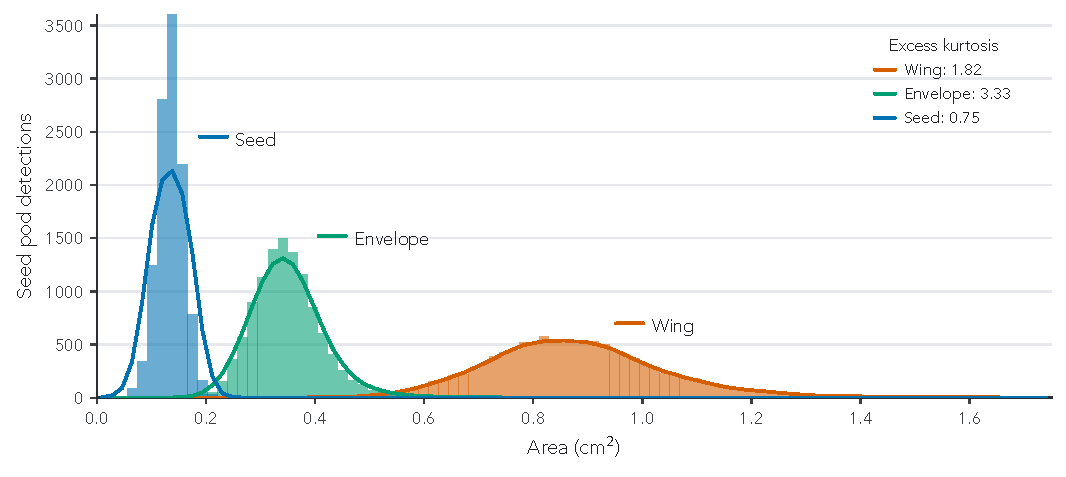
\includegraphics[width=\linewidth]{figures/pennycress-unet/area-distributions.pdf}
 \captionsetup{justification=raggedright,singlelinecheck=false}
 \caption[Distribution of seed-pod component areas]{Distribution of seed-pod component areas across non-empty population-scale detections. Histograms show the measured areas (cm$^2$) of wing, envelope, and seed tissues after excluding detections with zero watershed seed markers. Colored lines show five-bin moving averages of histogram counts, and inset values report excess kurtosis, quantifying heavier-than-normal distribution tails. Seed area is concentrated at smaller values, envelope area at intermediate values, and wing area at larger values; all three traits are right-skewed and log-normal-like, consistent with natural variation in plant morphology.}
 \label{fig:ch2-area-dist}
\end{figure}

\begin{figure}[!ht]
 \centering
 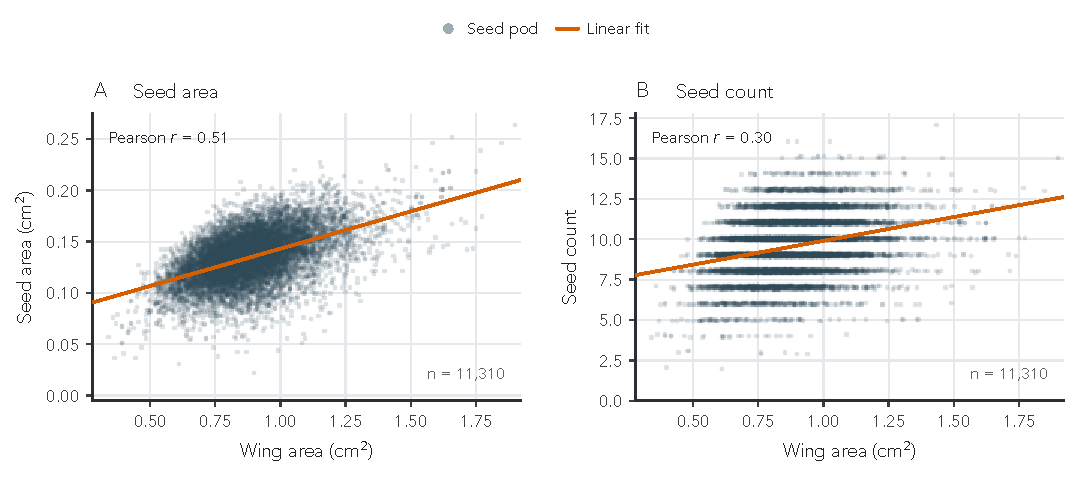
\includegraphics[width=\linewidth]{figures/pennycress-unet/wing-area-v-seed-area-count.pdf}
 \captionsetup{justification=raggedright,singlelinecheck=false}
 \caption[Relationships between wing area and seed traits]{Relationship between wing area and seed traits across non-empty population-scale detections. Wing area is plotted against (A) seed area and (B) seed count, with each point representing one seed pod and the solid line showing the linear least-squares fit. Points in (B) are vertically jittered by less than 0.1 seed for visibility; correlations and fitted lines use the unjittered seed-count values. Wing area is positively correlated with both seed area (Pearson $r = 0.51$) and seed count ($r = 0.30$), consistent with wing--seed regulatory association in \textit{Brassicaceae}.}
 \label{fig:ch2-wing-seed-corr}
\end{figure}

\subsection{Predictive Phenotype Network}
After extracting phenotypes from our dataset, we used iRF-LOOP to construct PPNs to check the biological plausibility of extracted phenotypes. Running iRF-LOOP on the entire dataset yielded a PPN with 48 nodes and 108 directed edges after filtering the network to include only the top 5\% of relationships (Figure~\ref{fig:ch2-pc-ppn}). Despite being a directed network, the PPN exhibited high reciprocity, indicating that predictive relationships tend to be mutual, which is expected for many geometrically derived traits.

\begin{figure}[p]
 \centering
 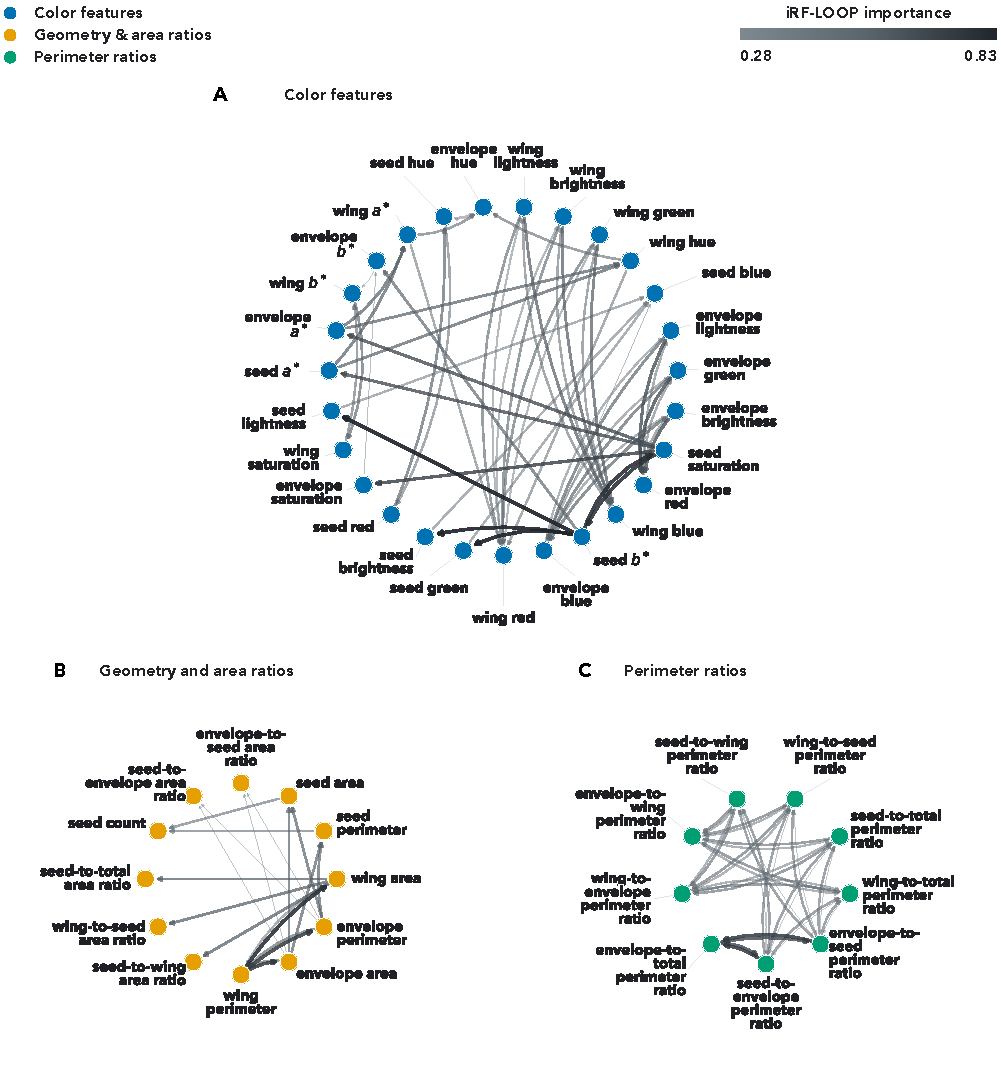
\includegraphics[width=\linewidth]{figures/pennycress-unet/pc-ppn-top0.05.pdf}
 \caption[Predictive phenotype network (PPN) for pod-related traits]{Predictive phenotype network (PPN) for pod-related traits after retaining the top 5\% of iterative Random Forest Leave-One-Out Prediction (iRF-LOOP) relationships. Nodes are measured phenotypes; node color and panel membership denote feature classes: (A) color features, (B) geometry and area ratios, and (C) perimeter ratios. Directed arrows indicate predictor-to-response relationships, and edge width and darkness encode iRF-LOOP importance. The filtered network contains 48 nodes and 108 directed edges. In color-feature labels, $a^*$ and $b^*$ are CIELAB color channels.}
 \label{fig:ch2-pc-ppn}
\end{figure}

The PPN separated into three connected components after filtering, each dominated by a single feature type: a 27-node component containing all color features across all three tissues, a 12-node component containing absolute geometry and area ratios, and a 9-node component containing all perimeter ratios. This separation by measurement type is expected given how tightly color and geometric features covary within each class.

To interpret the cross-tissue relationships more directly, we extracted the subset of PPN edges that connect traits across pod tissues (Figure~\ref{fig:ch2-pc-ppn-focus}). This focused subset separates two recurring patterns: pigment coupling among color traits and size coupling among envelope, seed, and wing geometry traits.

\begin{figure}[p]
 \centering
 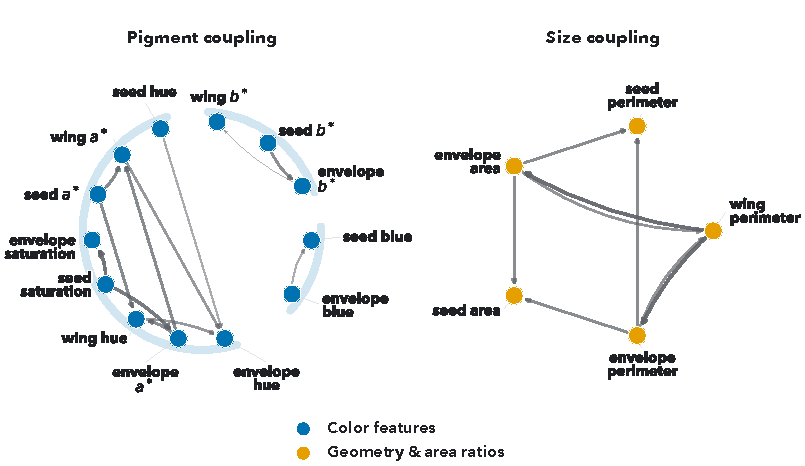
\includegraphics[width=\linewidth]{figures/pennycress-unet/pc-ppn-focus-subset.pdf}
 \captionsetup{justification=raggedright,singlelinecheck=false}
 \caption[Focused subset of cross-tissue predictive phenotype network relationships]{Focused subset of cross-tissue predictive phenotype network relationships. The subset highlights PPN edges connecting traits across pod tissues, separated into pigment coupling and size coupling groups. Nodes are measured phenotypes, with blue nodes denoting color features and orange nodes denoting geometry and area-ratio features. Directed arrows indicate predictor-to-response relationships, and edge width and darkness encode iRF-LOOP importance. Pale blue arcs visually group related pigment-feature relationships. In color-feature labels, $a^*$ and $b^*$ are CIELAB color channels.}
 \label{fig:ch2-pc-ppn-focus}
\end{figure}

Within this focused subset, several informative relationships emerged that could not be explained by geometric identities alone. Most notably, both envelope area and perimeter were predictive of seed area and perimeter (iRF-LOOP importance $\approx 0.56$), consistent with the pod's active role in seed development and resource allocation in \textit{Brassicaceae} \cite{wing-seed-assoc}. This relationship mirrors the envelope-to-seed area ratio, which was the most recurrent of our significant GWAS signals (Section~\ref{sec:ch2-gwas}). Similarly, seed and envelope color features were predictive of each other in CIELAB $b^*$, RGB blue, and HSV hue spaces. This suggests that color features, which provide a proxy for pod maturity and pigmentation, may be co-regulated across tissues. These relationships are correlative and do not imply causality, but they indicate that extracted phenotypes capture biologically coherent structure beyond trivial geometric relationships.

\subsection{Heritability of U-Net-Derived Pod Traits}
Of the 149 phenotypes available for this panel, 52 were extracted by our U-Net pipeline. Screening these for heritable genetic signal retained 34 traits, with $H^2$ ranging from 0.068 to 0.461 (Table~\ref{tab:ch2-heritability}); four of the 34 ultimately yielded significant GWAS associations.

Heritability was strongly structured by trait class. The 19 retained geometry and ratio traits spanned $H^2$ 0.188--0.461, whereas the 15 retained color traits spanned 0.068--0.321, and all seven of the most heritable traits were geometric. The most heritable color trait, wing HSV saturation ($H^2 = 0.321$), fell below every one of them. This separation anticipates the association results below, in which three of the four traits with significant hits are geometry or area ratios.

Heritability was necessary but not sufficient for a GWAS hit, and the retained set includes traits whose genotype variance components were weakly resolved. Fourteen of the 34 retained traits did not reach nominal significance on the restricted likelihood-ratio test ($p > 0.05$), and 12 of those 14 were color traits. Envelope-to-seed area ratio, which produced the most recurrent association signal, was itself borderline ($H^2 = 0.200$, $p = 0.0501$). We therefore treat the downstream candidates as exploratory rather than as well-powered genetic findings. Per-trait $H^2$ for all 52 U-Net-derived traits, including the 18 that fell below the screen, is reported in Table~\ref{tbl:heritability-all}.

\subsection{Genome-Wide Association and Gene Mapping}
We performed GWAS on the U-Net-derived pod traits on a panel of 189 accessions using four GAPIT models (MLM, MLMM, FarmCPU, and BLINK). We retained candidate SNPs with raw-$p < 1 \times 10^{-6}$ (a suggestive association cutoff; a Bonferroni threshold is overly stringent given linkage disequilibrium among SNPs) and MAF $\geq 0.03$, deferring false-positive control to GRIN filtering in the module derivation stage.

GWAS yielded six unique SNPs across four phenotypes: envelope CIELAB $b^*$, envelope-to-seed area ratio, wing area, and wing-to-seed area ratio. The most recurrent signal came from envelope-to-seed area ratio. Our GWAS results are summarized in Table~\ref{tab:ch2-gwas-results}.

\begin{table}[htbp]
 \centering
 \caption[Summary of retained GWAS associations for heritable, U-Net-derived pod traits]{Summary of retained GWAS associations for heritable, U-Net-derived pod traits (dryland environment), tested across 189 genotyped accessions. Associations are reported at a suggestive raw $p < 1\times10^{-6}$ cutoff; linkage disequilibrium among SNPs makes per-SNP tests non-independent, so a Bonferroni threshold is overly conservative. $H^2$, broad-sense heritability; SNPs, number of retained single nucleotide polymorphisms; Models, GAPIT models (MLM, MLMM, FarmCPU, BLINK) producing the associations; Lead SNP, most significant SNP (chromosome\_position); Lead raw $p$, its unadjusted $p$-value.}\label{tab:ch2-gwas-results}
 \small
 \setlength{\tabcolsep}{3.5pt}
 \renewcommand{\arraystretch}{1.1}
 \begin{tabularx}{\textwidth}{@{}>{\raggedright\arraybackslash}p{0.30\textwidth} c c >{\raggedright\arraybackslash}X l c@{}}
 \toprule
 Trait & $H^2$ & SNPs & Models & Lead SNP & Lead raw $p$ \\
 \midrule
 envelope CIELAB $b^*$
 & 0.217 & 1 & MLMM & \texttt{4\_8127381} & $8.71 \times 10^{-7}$ \\

 envelope-to-seed area ratio
 & 0.200 & 3 & BLINK, FarmCPU, MLMM & \texttt{5\_963442} & $1.04 \times 10^{-7}$ \\

 wing area
 & 0.366 & 1 & MLMM & \texttt{7\_63065229} & $4.14 \times 10^{-7}$ \\

 wing-to-seed area ratio
 & 0.285 & 1 & MLMM & \texttt{2\_2343404} & $6.06 \times 10^{-7}$ \\
 \bottomrule
 \end{tabularx}
\end{table}

We mapped the six retained SNPs from GWAS to pennycress genes using the mixed LD-decay and distance-based approach described in Section~\ref{sec:ch2-snp2gene}. For each SNP, we defined a window centered on the SNP with a width set by local LD-decay distance and assigned the annotated genes falling in that window, retaining any gene whose body directly contained that SNP. Windows spanned approximately $24.6$--$49.6$~kb, with strong LD-decay fits ($R^2 = 0.944$--$0.989$), reflecting the different recombination contexts of each chromosomal region. Because all six SNPs yielded reliable LD-decay fits, every candidate gene was assigned from an LD window, and the distance-based fallback was not used.

This procedure produced 69 candidate pennycress genes, with half of the loci tracing to the envelope-to-seed area trait and the remaining loci tracing to the other three GWAS traits. We mapped these genes to their nearest Arabidopsis orthologs in TAIR~\cite{garcia2002tair} to enable cross-species functional annotation and module derivation. This mapping yielded 64 unique orthologs, as several pennycress genes shared a single Arabidopsis ortholog. This ortholog set constitutes the candidate ortholog set carried forward to GRIN filtering and module derivation (Section~\ref{sec:ch2-mentor}).

\subsection{\textsc{Mentor} Module Derivation}
GRIN filtering reduced the candidate ortholog set of 64 genes to 33, pruning 31 that lacked sufficient network support; these 33 constitute the network-supported gene set. We applied \textsc{Mentor} to this set, using the process and standard settings described in Section~\ref{sec:ch2-mentor}, resolving it into three modules of 5, 11, and 17 genes (Figure~\ref{fig:ch2-mentor-dendro}). We then used these modules for mechanistic interpretation (Section~\ref{sec:ch2-mentor-ia}).

\begin{figure}[p]
 \centering
 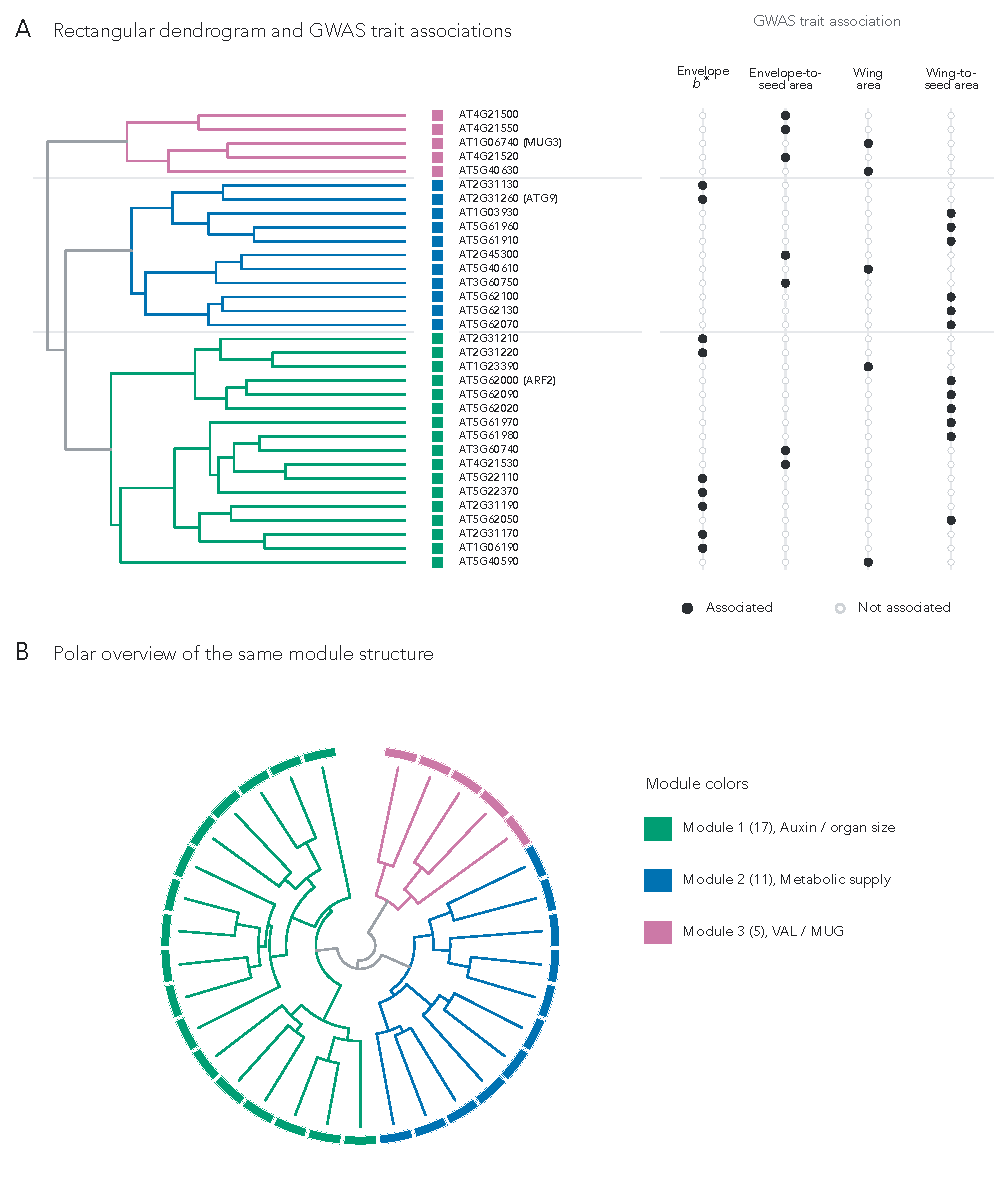
\includegraphics[width=0.96\linewidth,height=0.75\textheight,keepaspectratio]{figures/pennycress-unet/mentor-dendrogram.pdf}
 \caption[\textsc{Mentor} dendrogram of 33 candidate Arabidopsis orthologs retained from U-Net-derived pod traits]{\textsc{Mentor} dendrogram of the 33 GRIN-refined Arabidopsis orthologs retained from U-Net-derived pod-trait GWAS candidates. (A) Complete-linkage clustering of random-walk-with-restart (RWR) dissimilarities, with the adjacent trait matrix indicating which of the four GWAS traits---envelope CIELAB $b^*$, envelope-to-seed area ratio, wing area, and wing-to-seed area ratio---each gene was associated with. (B) Polar view of the same topology, emphasizing the three \textsc{Mentor} modules. Branch and outer-ring colors indicate Module 1 (17 genes; auxin, organ-size, and reproductive development), Module 2 (11 genes; metabolic supply, autophagy, and nutrient remobilization), and Module 3 (5 genes; VAL/MUG transposon-derived regulators).}
 \label{fig:ch2-mentor-dendro}
\end{figure}

\subsection{\textsc{Mentor-IA} Exploratory Interpretation}
We used \textsc{Mentor-IA} to conduct an exploratory interpretation of the three modules derived by \textsc{Mentor} (Section~\ref{sec:ch2-mentor}). Module 1, which contained 17 Arabidopsis orthologs, was run with the enrichment agent, literature agent, mygene interpreter, and meta aggregator. Module 2, which contained 11 orthologs, was run with the same agents as Module 1. Module 3, which contained 5 orthologs, was run with only the mygene interpreter and meta aggregator, as the small gene count limited the power of enrichment analyses. Because our modules did not have an associated network, we did not use the network agent for analysis.

\textsc{Mentor-IA} produced per-agent summaries for each module, along with a final interpretation that synthesized evidence across agents. This interpretation included keyword themes, enrichment statistics from GO and KEGG, and a mechanistic summary with candidate supporting citations. Across modules, the proposed mechanisms recovered known \textit{Brassicaceae} pod and seed biology, demonstrating our pipeline's ability to connect measured phenotypes to candidate mechanistic explanations. We manually cross-checked the agent output against pennycress and \textit{Brassicaceae} literature, finding the mechanistic summaries to be consistent with reported biology.

Because functional interpretation used Arabidopsis orthologs, the mechanisms below should be read as candidate hypotheses rather than validated pennycress-specific effects. For clarity, gene-symbol mentions below refer to Arabidopsis orthologs; parenthetical IDs give the Arabidopsis locus followed by the corresponding pennycress TAV2 locus or loci.

\subsubsection{Module 1 Interpretation}
We confirmed that the \textsc{Mentor-IA} module 1 analysis recovered mechanistic themes centered around auxin-mediated control of organ size and reproductive development, with supporting themes connecting to auxin and cell division more broadly. \cite{schruff2006} demonstrated that Arabidopsis \textit{ARF2} (\texttt{AT5G62000}; pennycress \texttt{TAV2\_LOCUS7857}) represses auxin-responsive transcription, limiting integument cell proliferation, and loss of \textit{ARF2} function leads to enlarged seeds and organs. \cite{paolo2021} found that \textit{ARF2} genetically interacts with \textit{SEEDSTICK} and \textit{GORDITA} during seed development, linking this auxin-response factor to integument growth and seed-coat differentiation. These findings provide the strongest candidate bridge to envelope-to-seed area ratio, while any connection to wing area remains more indirect through broader auxin-mediated organ-growth biology.

Module 1's link to auxin and cell division is further supported by the presence of Arabidopsis \textit{APC4} (\texttt{AT4G21530}; pennycress \texttt{TAV2\_LOCUS24640}), which encodes a subunit of anaphase-promoting complex (APC/C). \cite{wang2012apc4} demonstrated that Arabidopsis \textit{apc4} mutants exhibit defects in female gametogenesis and embryogenesis, with aberrant embryo cell division and distorted auxin distribution. \cite{liu2018arf} also implicated \textit{ARF2}, together with \textit{ARF4} and \textit{ARF5}, in gametophyte development, reinforcing the reproductive-development theme. Arabidopsis \textit{RUS2}/\textit{WXR1} (\texttt{AT2G31190}; pennycress \texttt{TAV2\_LOCUS13944}) provides a second auxin-related but less direct line of evidence. \cite{ge2010} showed that \textit{RUS2}/\textit{WXR1} is required for normal polar auxin transport and PIN/AUX1 abundance in roots, while \cite{leasure2009} placed \textit{RUS2} with \textit{RUS1} in a root UV-B-sensing pathway. Thus, the proposed \textit{RUS2} connection to wing growth is an inference from auxin-distribution biology rather than a demonstrated pod-morphology effect. The module also surfaced a possible connection to color phenotypes such as envelope CIELAB $b^*$; \textit{arf2} mutants show delayed senescence and altered chlorophyll retention in leaves \cite{ellis2005}. Because this evidence comes from leaves and developmental timing instead of pod-envelope color directly, the connection to pod color remains tentative.

In addition to the literature-supported themes that we manually verified, the \textsc{Mentor-IA} enrichment agent returned several significant GO and KEGG terms consistent with reproductive development, such as floral whorl development ($p = 9.8 \times 10^{-5}$), ovule development ($p = 3.6 \times 10^{-3}$), and embryo development ending in seed dormancy ($p = 3.6 \times 10^{-3}$), providing additional support for the proposed developmental theme.

Despite the strong theme and supporting evidence around auxin-mediated control of organ size and reproductive development, the remaining orthologs in module 1 had only gene-level annotation and no clear trait-linking literature in the \textsc{Mentor-IA} output, so we leave their exploration for future work and specify them as additional candidates. The module 1 interpretation is consistent with known biology of pod and seed development in \textit{Brassicaceae}.

\subsubsection{Module 2 Interpretation}
Module 2 is centered around metabolic supply, autophagy, nutrient remobilization, and chloroplast carbon metabolism. Unlike module 1, which provides evidence of a direct developmental regulator in \textit{ARF2}, module 2 provides an indirect hypothesis in which metabolic supply from the pod to the seed may influence pod growth. The strongest candidate connection is to envelope-to-seed area ratio and pod filling because the literature links these pathways to seed resource allocation rather than directly to pod morphology.

Arabidopsis \textit{ATG9} (\texttt{AT2G31260}; pennycress \texttt{TAV2\_LOCUS12330}) anchors the module's autophagy signal. \cite{shin2014} showed that \textit{ATG9} contributes to autophagic flux, while \cite{inoue2006} found that \textit{atg9} mutants retain constitutive autophagy in root tips, supporting a modulatory role instead of a strictly essential one. \cite{kang2018} and \cite{luo2023} place \textit{ATG9} in autophagosome formation and closure pathways, and \cite{lai2020} provides structural evidence for \textit{ATG9}'s role in autophagy via cryo-EM, showing that it is the core integral membrane autophagy protein. \cite{guiboileau2012} observed that \textit{atg} mutants show reduced nitrogen remobilization to seeds under both low- and high-nitrate conditions, and \cite{diberardino2018} demonstrated that autophagy affects resource allocation and storage-protein accumulation during seed development. These findings suggest that variation in autophagy may affect pod filling or envelope-to-seed nutrient allocation, providing a candidate link to phenotypes like envelope-to-seed area ratio.

Arabidopsis \textit{TKL1} (\texttt{AT3G60750}; pennycress \texttt{TAV2\_LOCUS16016}) provides a second line of evidence for metabolic supply and chloroplast carbon metabolism. \cite{rocha2014} found that \textit{TKL1} is phosphorylated at Ser428 in a light- and chloroplast-dependent manner, suggesting that it may be a regulatory point for carbon flux in the Calvin-Benson-Bassham (CBB) cycle and oxidative pentose phosphate pathway (OPPP). Additionally, \cite{khozaei2015} demonstrated that altered plastid transketolase dosage disrupts growth through thiamine- and TPP-related metabolic constraints. Because carbon supply is important to seed growth, we infer that \textit{TKL1} may provide a second, indirect link to pod growth and envelope-to-seed area, supporting our mechanistic supply hypothesis.

Additionally, \cite{shen2006} adds a redox-homeostasis line of evidence, showing that Arabidopsis \textit{GPDHc1} (\texttt{AT5G40610}; pennycress \texttt{TAV2\_LOCUS25599}) controls plant NADH/NAD\textsuperscript{+} ratios through the mitochondrial glycerol-3-phosphate shuttle. Although the OPPP is not directly implicated in this work, it supports a broader interpretation in which module 2 captures genes involved in carbon and redox balance during pod and seed development.

Outside of the autophagy and metabolic supply themes, the remaining module 2 genes had only gene-level annotation and no clear trait-linking literature, so we specify them as additional candidates for future exploration. Overall, the module 2 interpretation is consistent with known biology of seed filling and envelope-to-seed biomass allocation, providing a plausible but indirect mechanistic hypothesis connecting our phenotypes to metabolic supply and autophagy.

\subsubsection{Module 3 Interpretation}
Since module 3 yielded only sparse gene-level annotation and lacked enrichment and literature support, we did not advance a mechanistic interpretation for it; its genes remain candidates for future analysis.

\subsubsection{Expression-Based Plausibility Check}
We further evaluated the plausibility of our candidate mechanisms by examining gene expression in pennycress leaf, pod, and root tissues using the dataset from \cite{combsgiroir2024waterlogging}. For the purpose of connecting candidate genes to pod phenotypes, we focused on expression in pod tissues. The strongest literature-supported candidate loci were expressed in pods. These included the module 1 candidates \textit{ARF2} (\texttt{TAV2\_LOCUS7857}), \textit{APC4} (\texttt{TAV2\_LOCUS24640}), and \textit{RUS2} (\texttt{TAV2\_LOCUS13944}), and the module 2 candidates \textit{ATG9} (\texttt{TAV2\_LOCUS12330}), \textit{TKL1} (\texttt{TAV2\_LOCUS16016}), and \textit{GPDHc1} (\texttt{TAV2\_LOCUS25599}). By contrast, several lower-priority candidate loci were not highly expressed in pod tissues. The \textit{BAG2} orthologs were \texttt{TAV2\_LOCUS6658} and \texttt{TAV2\_LOCUS26197}. The \textit{bHLH010} ortholog was \texttt{TAV2\_LOCUS13948}; the \textit{bHLH091} orthologs were \texttt{TAV2\_LOCUS13945} and \texttt{TAV2\_LOCUS13946}. These lower expression patterns support our focus on the literature-backed mechanisms. The sparse expression of many module 3 paralogs also supports treating that module as a future-work candidate set. Overall, expression results indicate that prioritized candidates are active in pod tissues, supporting their plausibility as candidate mechanisms and providing a basis for future experimental validation.

\begin{figure}[p]
 \centering
 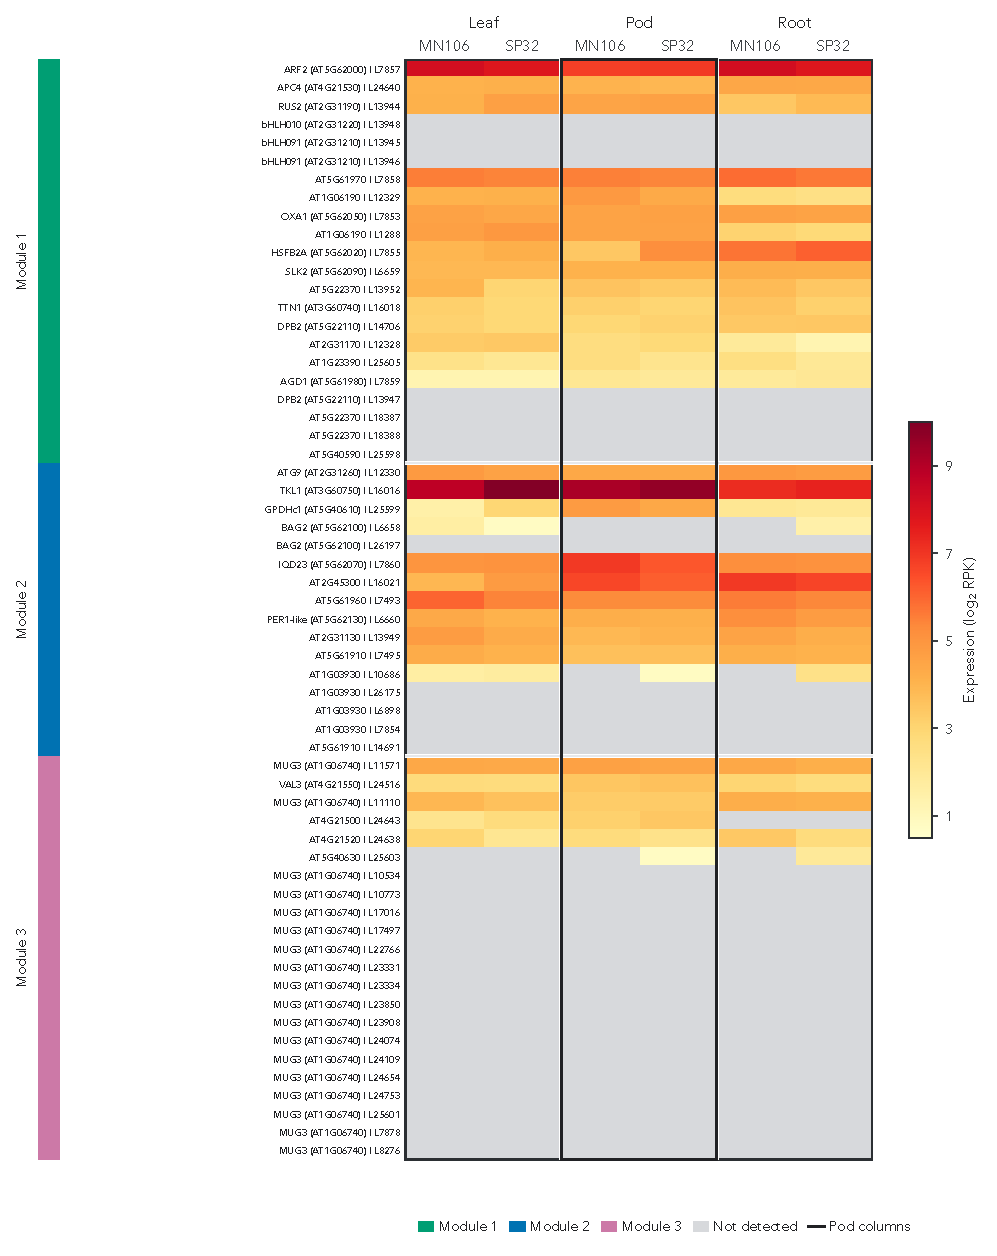
\includegraphics[width=\linewidth,height=0.76\textheight,keepaspectratio]{figures/pennycress-unet/pod-expression-heatmap.pdf}
 \captionsetup{justification=raggedright,singlelinecheck=false}
 \caption[Expression of \textsc{Mentor}-derived candidate loci across pennycress tissues]{Expression of \textsc{Mentor}-derived candidate loci across pennycress tissues. Rows are pennycress loci grouped by \textsc{Mentor} module; repeated Arabidopsis orthologs reflect paralogous pennycress loci. Cell color encodes log$_2$-transformed expression (reads per kilobase) in leaf, pod, and root tissue for MN106 and SP32, with gray cells denoting values below the detection threshold ($\leq 0.5$). Pod columns are grouped and outlined because the candidate-gene plausibility assessment focuses on pod expression, and bold row labels mark literature-supported candidates emphasized in the text.}
 \label{fig:ch2-combined-expression}
\end{figure}

\section{Discussion}
We found that a custom U-Net provided the most favorable accuracy-efficiency tradeoff among the benchmarked CNN, transformer, and foundation model architectures when training and testing on our open-source, hand-annotated ground truth dataset of 347 seed pod images. These results suggest that for small, specialized biological datasets like ours, a task-specific CNN with tailored inductive biases can match or modestly exceed more complex architectures while requiring less computation. However, we note that our small dataset size and tiling scheme may have limited the performance of transformer- and foundation model-based architectures, which rely on large receptive fields and pretraining priors. Future work could explore whether larger datasets and different preprocessing strategies can unlock the potential of these architectures for pennycress phenotyping.

Our pipeline produced 52 biologically plausible, tissue-resolved phenotypes at population scale (12,253 seed pods over 768 accessions). Deep learning methods provided a 30- to 45-fold speedup over manual annotation while achieving 85.58\% mIoU. Extracted seed, wing, and envelope areas exhibited a log-normal distribution, wing area was positively correlated with seed area and count, and the resulting PPN separated into coherent color, geometry, and perimeter sub-networks while highlighting cross-tissue pigment and size coupling. These results indicate that our pipeline may enable new avenues for research on pennycress seed pod biology through accurate and fast high-throughput measurements.

Starting from our image-derived pod traits, our pipeline surfaced candidate genes and mechanisms that recover known \textit{Brassicaceae} pod and seed biology. GWAS yielded significant associations for four pod traits, which we mapped to 69 pennycress genes and 64 Arabidopsis orthologs. GRIN narrowed these to 33 network-supported candidates, which \textsc{Mentor} resolved into three modules; two were related to pod and seed biology. Module 1 was the strongest, centered on auxin-mediated organ growth, reproductive development, and cell division. Its key gene, \textit{ARF2}, offers the clearest candidate bridge to envelope-to-seed area. Module 2 was more indirect: autophagy, nutrient remobilization, and redox balance via \textit{ATG9}, \textit{TKL1}, and \textit{GPDHc1} support a plausible metabolic-supply hypothesis for pod filling and envelope-to-seed allocation. However, these candidates rest on Arabidopsis orthologs, as pennycress network and literature data remain limited.

We compared the \textsc{Mentor-IA} results to pennycress gene expression data, using the expression heatmap to assess hypothesis plausibility in pod tissues. Prioritized Module 1 and 2 candidates were expressed in pods, while some lower-priority candidates were weakly expressed or not detected, supporting our focus on the literature-backed mechanisms. Furthermore, Module 3 expression is sparse, supporting our decision to treat it as a candidate set for future work. It is important to note that expression was measured across the whole pod and is correlative, so it does not establish causality or eQTL regulation. However, our expression evidence supports prioritization of our literature-backed candidates for future studies.

Despite this progress, our work has some limitations. Collecting and scanning seed pods to use for segmentation is still a labor-intensive process; this could become a bottleneck in future population-scale studies, and it only yielded a small training set. Additionally, the model's performance is dependent on the quality of label data due to its supervised nature. Accurately annotating seed border pixels was difficult due to the low brightness and contrast levels in image scans, and this limitation was reflected in the lower accuracy for seeds than other surfaces. Furthermore, benchmark compatibility with nnU-Net is imperfect due to its built-in adaptive preprocessing and evaluation pipeline.

Additionally, GWAS results are limited as they used only 189 accessions and retained SNPs with a permissive threshold, although GRIN did help filter candidates further. Due to the limited availability of pennycress data, we relied on Arabidopsis orthologs for module derivation and interpretation, which may not fully capture pennycress biology. Finally, the \textsc{Mentor-IA} interpretation is exploratory and based on literature evidence from Arabidopsis, so it must be experimentally validated in pennycress to draw strong conclusions.

We present several avenues for future work to extend this pipeline. Improving imaging quality and scanning throughput could yield higher-quality datasets, which can also be expanded through more hand annotation for ground truth. Additionally, performing GWAS on a larger panel of accessions can provide higher-powered association results. Finally, experimental validation of the candidate mechanisms, such as \textit{ARF2}/\textit{APC4}/\textit{RUS2} and \textit{ATG9}/\textit{TKL1}/\textit{GPDHc1}, can test their relevance to pennycress pod phenotypes and provide a deeper understanding of the underlying biology.

This work has several implications for future pennycress research. We found no prior work that extracts intensive phenotypes from pennycress seed pods due to the labor-intensive nature of this task. Therefore, this article provides a novel pipeline for extracting several biologically important phenotypes at the population scale for pennycress and linking them to genetic variants. The framework allows scientists to perform experiments on pennycress that were previously impossible; for example, researchers can examine how treatments and experimental conditions affect entire populations by measuring seed pod phenotypes across treatment groups. Furthermore, scientists can test hypotheses about phenotypic relationships on a broad scale, leading to higher-impact research. More broadly, this work shows how deep learning-derived phenotypes can be carried into genetic association and module-level interpretation to prioritize table biological hypotheses.

    \chapter{Deep Learning for Genotype-by-Environment Prediction of Maize Grain Yield}\label{ch3:gxe}

\section{Introduction}
Genotype-by-environment (G$\times$E) interactions are a key mechanism underlying crop stability and performance \cite{lopez2023leveraging,rogers2021importance}. Accurately modeling these interactions has important practical implications, including increased food security and optimized farming practices \cite{ray2013yield}. Because the G$\times$E contribution to grain yield variation is substantial, yield rankings are not stable across environments; a hybrid superior in one site or year may be inferior in another \cite{rogers2021importance,lopez2023leveraging}. A breeder who selects on cross-environment mean performance will systematically mis-rank hybrids for the environment of interest. Therefore, predicting within-environment hybrid ordering is critical for improved selection. 

An increase in publicly available data has brought both renewed focus and challenge to G$\times$E prediction. The Genomes to Fields (G2F) Initiative curated a public dataset of genotypes and environments, which spans multiple years, hybrids, and field sites \cite{lopez2023leveraging}. Each yield observation carries both the genotype and the environmental covariates of the plot it was grown in, so a model can represent G$\times$E interactions directly. The 2024 G2F prediction competition built a benchmark on this dataset and standardized the task with a common dataset \comment{repeats the word "dataset"}, a held-out target year, and a single evaluation metric \cite{g2f-2024-competition}. This design makes independently developed methods directly comparable. The competition scores predictions by the Pearson correlation within each environment \comment{well, technically only the 2025 comp (manuscript in prep) did}, averaged across environments, which gives relative ranks priority over absolute scale \cite{g2f-2024-competition}. Additionally, since this dataset was collected in real-world field conditions, it contains heterogeneous data sources with varying quality and extensive missingness. By addressing these constraints, models developed on this dataset are more likely to generalize to real-world breeding scenarios.

A variety of methods have been developed for G$\times$E prediction. Early genomic prediction approaches relied on statistical models such as genomic best linear unbiased prediction (GBLUP) \cite{vanraden2008efficient} and Bayesian linear mixed models \cite{meuwissen2001prediction} to predict breeding values purely from genotypes. These methods were later extended to add genotype-by-environment covariance structure, either through explicit modeling of environmental covariates \cite{crossa2017genomic,heslot2014integrating} or kernel-based approaches \cite{jarquin2014reaction}. Although these methods have proven effective for G$\times$E prediction in some scenarios, they are limited by several inductive biases. The interaction structure must be specified a priori in the case of kernel methods, which prevents flexible modeling of complex relationships. Furthermore, these methods assume a linear relationship between inputs and outputs, which limits the depth of interactions that can be learned. In the case of G$\times$E prediction, this is particularly limiting because the relationship between genotype and environment is often nonlinear \cite{montesinos2021review}.

By contrast, deep learning models are a natural extension for multimodal genomic prediction because they can learn nonlinear feature hierarchies from heterogeneous inputs \cite{azodi2019benchmarking,montesinos2024multimodal}. Prior studies have applied multilayer perceptrons (MLPs) to compute structured interaction components \cite{montesinos2018multi}, combined genotype and weather data to predict yield directly \cite{shook2021crop}, and used sequence models, including state-space and transformer architectures, to model marker sequences \cite{caduceus,snvformer,wu2023transformer}.

However, when a wide range of modeling strategies were evaluated head-to-head in the first public G2F prediction competition, which used the 2022 season as its held-out target, statistical and deep learning models both produced satisfactory yield estimates with no family separating decisively from the rest \cite{g2f-maize-2025}. This result suggests that no single model class guarantees better accuracy on this task. Multimodal architectures for genomic prediction commonly encode each modality with its own encoder and combine the resulting representations late, through concatenation, a weighted sum, or a dedicated fusion layer \cite{montesinos2024multimodal, shook2021crop}. Under this paradigm, marker--environment interactions can only be formed after each modality has been processed independently, so the interactions available to the model are limited to those that survive compression. This design leaves an open question: whether direct interactions between individual marker and environmental tokens improve G$\times$E prediction \comment{if we say "open question", do we need to formulate the next clause as a question? otherwise, I feel like it kinda reads oddly}.

We designed this study to test whether a unified marker and environment representation could outperform branch-based late fusion for G$\times$E prediction. We trained the FullTransformer \comment{this is the first time mentioning "the FullTransformer," need to introduce it properly} with the 2024 G2F competition data and encoded marker and environmental tokens in one transformer sequence \cite{g2f-2024-competition,attention}. A sparse MoE block supported token-level specialization, and an affine head corrected absolute scale while it preserved within-environment rank. We reviewed 427 run records and selected completed comparisons of fusion architecture, objective choice, and affine calibration. The selected model achieved a macro environment PCC of $0.423$ and MSE of $55.40$; this result corresponds to sixth place in the retrospective comparison. Future work will test whether new data and feature representations can close the gap to the competition-winning PCC of $0.45$ \comment{after disqualification, comp winning number is now 0.436, and we would be third place}.

\section{Methods}
\subsection{Data}
Data for this model were obtained through the 2024 Genomes to Fields (G2F) Maize Prediction Competition \cite{g2f-2024-competition}. The dataset included trait, metadata, soil, weather, genotype, and environmental covariate files spanning the 2014-2024 growing seasons, with yield labels for 2014-2023 released prior to the competition, and 2024 labels made publicly available after the competition's end. The training dataset contained 173,960 trait rows across 272 environments; 164,921 of those rows had finite yield. The 2024 test dataset contained 10,057 submission-template rows across 23 environments. Raw genotype data contained 5,899 hybrid records with 2,425 single nucleotide variant (SNV) marker loci. Environmental data contained 654 numeric environmental covariates (ECs), along with 16 daily weather variables and separate metadata and soil tables. 

The data were collected across many sites, years, and management regimes, so they are heterogeneous and carry extensive missingness. The competition organizers deliberately released much of the data in raw form to capture the difficulty of modeling real-world data. Extensive preprocessing, including filtering and imputation, was necessary to address inconsistencies and ensure reliable performance. We detail the steps taken to clean our marker and environmental data in Sections~\ref{sec:ch3-marker-preproc} and~\ref{sec:ch3-env-preproc} respectively.

\subsubsection{Marker Data}\label{sec:ch3-marker-preproc}
The raw numerical genotype table contained 5,899 hybrid records and 2,425 candidate SNV loci. The raw marker files stored these states as $0$, $0.5$, and $1$, so at each locus, we encoded alleles by dosage according to the scheme in Table~\ref{tab:ch3-vocabulary} to make them compatible with tokenization. A value of $2$ represents two major alleles, a value of $1$ represents a heterozygous pair of alleles (major-minor), and a value of $0$ represents two minor alleles. 

\begin{table}[htbp]
    \centering
    \renewcommand{\arraystretch}{1.5}
    \begin{tabular}{@{} l c @{}}
        \toprule
        \textbf{Allele Combination} & \textbf{Model Token} \\
        \midrule
        Major-Major (\textit{AA}) & 2 \\
        Major-Minor (\textit{Aa}) & 1 \\
        Minor-Minor (\textit{aa}) & 0 \\
        \bottomrule 
    \end{tabular} 
    \caption{Genomic Input Marker Encodings. Each diploid marker is encoded as a single token representing the dosage of the major allele by multiplying the raw dosages ($0$, $0.5$, $1$) by two.}
    \label{tab:ch3-vocabulary}
\end{table}

Marker data preprocessing consisted of filtering and imputation, which we applied to the released all-hybrid genotype table. We removed loci with more than $10\%$ missing values. This process removed 201 loci, leaving 2,224 locus inputs to our final model. Additionally, phenotype rows without a corresponding genotype were dropped, decreasing the training set from 164,921 to 163,026 rows.

For the reported model, missing marker calls were processed sequentially in genotype-file order. For each missing call, we calculated the locus-specific median among genotype records sharing either parent with the target hybrid. Missing loci were replaced with the corresponding median value. Because records were processed sequentially, values imputed for earlier records could contribute to the donor medians used for later records. In total, this procedure filled 104,820 missing calls. After imputation, dosage values were multiplied by two and rounded to the nearest integer to produce model tokens. This conversion affected 2,516 imputed calls whose values fell outside the raw $\{0, 0.5, 1\}$ dosage grid; ordinary heterozygous calls at $0.5$ converted exactly to token $1$.

\subsubsection{Environmental Data}\label{sec:ch3-env-preproc}
In addition to genotypic data, we cleaned environmental data in a multi-step process. First, we focused on the output column, which measured grain yield in megagrams per hectare (Mg/ha) and served as the prediction target. We excluded all rows which lacked either yield measurements or complete environmental data. Of the 173,960 raw trait rows, 9,039 lacked a finite yield value and were dropped. From the 163,026 rows that retained both a finite yield and a matching genotype record (Section~\ref{sec:ch3-marker-preproc}), we further removed rows without seasonal weather data, yielding 161,803 records, and rows without EC coverage, yielding 143,050 records. These plot records corresponded to 238 unique environments. Because 34 environments lacked complete weather or EC blocks, they were excluded from the final cohort.

After applying these filters, we performed imputation on the weather station location data included in the competition dataset. For weather stations with partially missing data, we replaced missing observations with the station's mean latitude/longitude coordinates over all existing years. One research station, location TXH4, had no location data present. We used the Texas Tech New Deal Research farm \cite{txh4} as a proxy to retrieve the coordinates for this station, since both are located in Lubbock, Texas. We used the facility's official website to retrieve the New Deal Research Farm's latitude and longitude.

In addition to imputing weather-station locations, we compressed the daily weather data into 46 summary features. First, we indexed the 16 daily weather variables by environment and date, and dropped five variables \comment{which 5 variables? why?}, reducing the daily weather set to 11. We then aggregated variables starting on the planting date, and ending 14 days after harvest for historical environments and on the last date supplied in the seasonal-weather record for 2024 environments. For each retained weather variable, we calculated the minimum, maximum, mean, and accumulated sum over the aggregation window, yielding 44 summary features. We added the starting month and number of included days as additional features.

Following filtering and imputation, we integrated our location, weather, and environmental covariate datasets into a unified set of 705 variables, which consisted of 654 ECs, 46 weather summaries, two coordinates, and three categorical fields. In the best run, the three categorical fields (\texttt{Irrigated}, \texttt{Treatment}, and \texttt{Previous\_Crop}) were excluded, leaving 702 numeric environmental covariates as model inputs. Continuous variables were standardized to zero mean and unit variance, and the scaler was fit only on the training set to prevent data leakage.

We applied the same coverage requirements to the 2024 benchmark rows. Of the 10,057 submission-template rows across 23 environments, 9,486 rows across 22 environments entered the benchmark cohort. The filters removed all 385 rows of environment \texttt{SCH1\_2024}, so that environment does not appear in the cohort or in any reported benchmark result. The remaining 186 excluded rows came from 13 environments that were retained.

\subsection{Model Architecture}\label{sec:ch3-architecture}
\subsubsection{Overview}
We developed the FullTransformer, a full-sequence transformer model that predicts maize yield as a function of genotype and environment. The model represents marker dosages and environmental covariates in one token sequence, allowing self-attention to model genotypic, environmental, and G$\times$E structure in a shared representation space. A sparse mixture-of-experts (MoE) feed-forward sublayer \cite{shazeer2017outrageously} adds capacity through token-level expert routing, and a learned \texttt{[CLS]} summary token \cite{bert} provides the representation used for rank prediction. An environment-conditioned affine-calibration branch converts the rank prediction into the final yield estimate. The architecture is summarized in Figure~\ref{fig:ch3-fullarch}.

\begin{figure}[t]
    \centering
    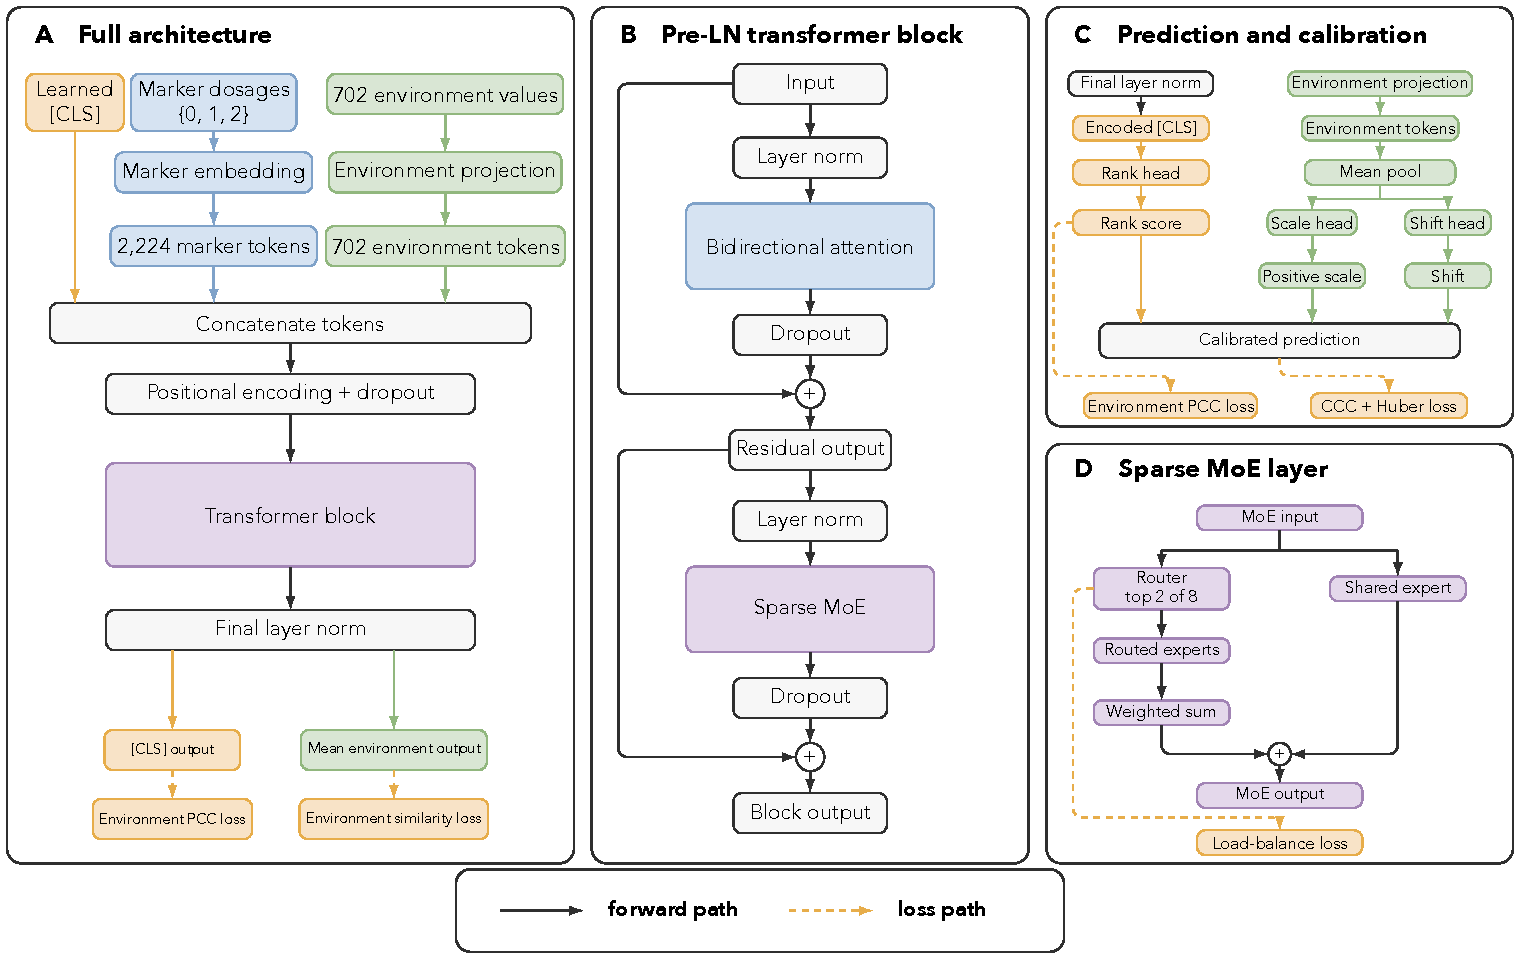
\includegraphics[width=\linewidth]{figures/gxe-tf/fulltransformer-architecture.pdf}
    \caption{ \comment{this fig shows up after all the prose. Any way to move it up? Let's also remove the box around the legend.} FullTransformer architecture for maize yield prediction. (A) The model embeds 2,224 marker dosages and projects 702 environmental values into one sequence with a learned \texttt{[CLS]} token. One transformer block produces the normalized \texttt{[CLS]} and environmental representations used by the primary and auxiliary losses. (B) The pre-layer-normalized block applies bidirectional attention and a sparse MoE layer with dropout and residual connections. (C) \comment{i think that A) and C) are slightly misaligned here in terms of how they convey the environmental input} The rank head predicts relative yield, while the mean projected environmental representation supplies a positive scale and shift for affine calibration. The environment PCC loss acts on the rank score, and the CCC and Huber losses act on the calibrated prediction. (D) \comment{maybe have dotted lines from the MoE block in B) indicating the "expanded" view of the MoE} The MoE router selects two of eight routed experts per token and combines their weighted output with one shared expert. A load-balance loss discourages routing collapse. Blue blocks show marker and attention operations, green blocks show environment operations, purple blocks show MoE operations, and orange blocks show \texttt{[CLS]} and losses. Solid arrows show forward paths, and dashed arrows show loss paths.}
    \label{fig:ch3-fullarch}
\end{figure}

\subsubsection{Input Representation}
For the reported model, each sample was represented by a sequence of length $2{,}927$: one learned \texttt{[CLS]} summary token, 2,224 marker tokens, and 702 environmental tokens. Marker dosages in $\{0,1,2\}$ were embedded with a shared learned lookup table of vocabulary size three and width 256. The same learned \texttt{Linear(1,256)} projection was applied to every standardized environmental scalar, producing one token per environmental feature. The \texttt{[CLS]}, marker, and environmental tokens were concatenated in that order, and a static sinusoidal positional encoding \cite{attention} was added to the sequence. This produced a per-sample encoder input of shape $2{,}927 \times 256$.

Because yield prediction depends on the complete input rather than autoregressive next-token prediction, no causal attention mask was applied. Bidirectional attention \cite{bert} allowed every marker and environmental token to attend to every other position, enabling direct marker--environment interactions within the shared representation.

\subsubsection{Transformer Encoder with Mixture-of-Experts}
The reported FullTransformer used one encoder block with hidden width $256$ and four bidirectional attention heads. The block followed the pre-layer-normalized residual organization used in GPT-2 \cite{gpt2}, with layer normalization applied before each sublayer \cite{layernorm}. The normalized token representations were passed through multi-head self-attention, and dropout with rate $0.15$ was applied to the attention output before it was added to the block input through a residual connection \cite{he2016deep}. The updated token representations were normalized again and passed through the MoE sublayer, whose output received the same dropout before the second residual addition.

The reported encoder replaced the conventional dense feed-forward sublayer with a sparse MoE layer \cite{shazeer2017outrageously}. A learned linear router produced eight logits, one for each routed expert, for every sequence token, including \texttt{[CLS]}, marker, and environmental tokens. The two routed experts with the highest logits were selected independently for each token, and a softmax over those logits produced weights used to combine their outputs. Each routed expert was a two-layer FFN with hidden width $256$, GELU activation, and output width $256$. An additional shared expert with the same structure processed every token, and its output was added to the weighted sum of routed-expert outputs. During training, an auxiliary load-balancing loss with weight $0.01$ discouraged routing collapse by encouraging routing mass to remain distributed across the eight routed experts. This design increased conditional capacity while activating only two routed experts, in addition to the shared expert, for each token. \comment{should we add that this block is visualized in figure 1?}

\subsubsection{Prediction and Calibration Heads}
After the final transformer block, layer normalization was applied to the full sequence. The normalized representation at the \texttt{[CLS]} position was passed through a \texttt{Linear(256,1)} head to produce a scalar rank prediction. This rank head was optimized directly against the environment PCC loss described in Section~\ref{sec:ch3-training}.

The selected model additionally applied an environment-conditioned affine calibration to transform the rank prediction into an absolute-yield prediction. For each sample, we took the mean of its 702 projected environmental input tokens, computed before positional encoding and transformer processing. Every plot record within one environment carried the same environmental covariates, so this mean was constant within an environment; we therefore write it as $\bar{\mathbf z}_E$ for environment $E$. Two learned \texttt{Linear(256,1)} heads, $f_s$ and $f_b$, mapped $\bar{\mathbf z}_E$ to a scalar raw-scale value and a scalar shift, respectively. The calibrated total prediction was computed as

\begin{equation}\label{eq:ch3-affine-calibration}
    \begin{aligned}
        s_E^{\mathrm{raw}} &= f_s(\bar{\mathbf z}_E), &
        b_E &= f_b(\bar{\mathbf z}_E), &
        f_s,f_b &: \mathbb{R}^{256} \rightarrow \mathbb{R}, \\
        \hat{y}_{\mathrm{total}}
        &= \left[\operatorname{softplus}\!\left(s_E^{\mathrm{raw}}\right)+10^{-4}\right]
        \hat y_{\mathrm{rank}} + b_E.
    \end{aligned}
\end{equation}

The weights of both calibration heads and the bias of the shift head were initialized to zero. The scale-head bias was initialized to the inverse softplus of one, so the initial scale was approximately $1.0001$ after adding the $10^{-4}$ offset, while the initial shift was zero. The softplus activation and offset constrained the scale to be strictly positive. Every hybrid in the same environment shared the same positive scale and shift, so calibration preserved both the within-environment rank ordering and Pearson correlation, leaving the macro environment PCC unchanged while allowing adjustment of absolute yield scale.

The model also exposed the mean of the encoded environmental tokens after the transformer and final normalization for use in the auxiliary environment-similarity loss (Section~\ref{sec:ch3-losses}). This pooled representation was not itself a prediction head; it shaped the learned environmental representation as described below.

\subsection{Training}\label{sec:ch3-training}
\subsubsection{Training Objective}\label{sec:ch3-losses}
The training objective was built around an environment PCC loss designed to mirror the competition's macro environment PCC metric. Within each local per-GPU microbatch, we computed the Pearson correlation between observed yield and the model's rank prediction for every environment $e \in \mathcal{E}_B$ containing at least four observations. Here, $\hat{y}_i$ denotes the rank prediction for sample $i$. Each GPU computed correlations from its local microbatch of 256 samples, and the sufficient statistics were not pooled across GPUs. The raw environment correlations were uniformly averaged without Fisher $z$ transformation or sample-count weighting. The environment PCC loss was defined as

\begin{equation}\label{eq:ch3-pcc}
    r_e =
    \frac{\sum_{i \in e} (y_i - \bar{y}_e)(\hat{y}_i - \bar{\hat{y}}_e)}
    {\sqrt{\sum_{i \in e}(y_i - \bar{y}_e)^2}
     \sqrt{\sum_{i \in e}(\hat{y}_i - \bar{\hat{y}}_e)^2}}.
\end{equation}

\begin{equation}\label{eq:ch3-envpcc}
    L_{\mathrm{envpcc}} = 1 - \frac{1}{|\mathcal{E}_B|} \sum_{e \in \mathcal{E}_B} r_e.
\end{equation}

In addition to optimizing within-environment ranking, we implemented an auxiliary environment-similarity objective to align internal environmental representations with the raw environmental data. We mean-pooled the encoded environmental tokens into an embedding $\mathbf{z}_i$ for each sample $i$. The cosine similarity between $\mathbf{z}_i$ and $\mathbf{z}_j$ defined the learned similarity $S^{z}_{ij}$, while the cosine similarity between their standardized raw environmental vectors defined the target similarity $S^{E}_{ij}$. We computed the loss as the mean-squared difference between these similarities over all off-diagonal pairs in a local microbatch of size $B$:

\begin{equation}\label{eq:ch3-env-sim}
    L_{\mathrm{env\text{-}sim}} = \frac{1}{B(B-1)} \sum_{\substack{1 \leq i,j \leq B \\ i \neq j}} (S^{z}_{ij} - S^{E}_{ij})^2 .
\end{equation}

The maximum weight of this loss was $0.1$. The term was inactive until epoch 50 and then ramped linearly to its maximum weight by epoch 100.

For absolute-yield calibration, the calibrated total prediction was optimized with an environment concordance correlation coefficient (CCC) loss \cite{lin1989concordance} and a mean Huber loss \cite{huber1964robust}. For each environment $e$, the concordance correlation was

\begin{equation}\label{eq:ch3-ccc-loss}
\begin{aligned}
    \rho_{c,e}
    &= \frac{2\,\operatorname{cov}\!\left(y_e,\hat{y}^{\mathrm{total}}_e\right)}
    {\sigma_{y,e}^{2}+\sigma_{\hat{y}^{\mathrm{total}},e}^{2}
    +\left(\mu_{y,e}-\mu_{\hat{y}^{\mathrm{total}},e}\right)^2}, \\
    L_{\mathrm{envCCC}}
    &= 1-\frac{1}{|\mathcal{E}^{(2)}_B|}
    \sum_{e \in \mathcal{E}^{(2)}_B}\rho_{c,e},
\end{aligned}
\end{equation}

where $\mathcal{E}^{(2)}_B$ contained environments in the local microbatch with at least two observations and nonzero yield and prediction variance. The environment CCC loss had maximum weight $0.05$. The Huber loss used mean reduction, $\delta=1.0$, and maximum weight $0.02$. Both calibration terms were inactive until epoch 150 and ramped linearly to their full weights by epoch 250. Until epoch 250, the rank prediction was detached from calibration gradients \comment{what does this mean?}, allowing the calibration heads to learn without altering the rank head. Beginning at epoch 250, calibration gradients reached the rank prediction at $10\%$ of their ordinary magnitude \comment{this is just a weight of 0.1, think that would be clearer to say}, while the environment PCC loss on the rank prediction remained fully active throughout training.

Combining all of these objectives, the total loss function was defined as

\begin{equation}\label{eq:ch3-total-loss}
    L(t) = L_{\mathrm{envpcc}}
    + 0.1\,r_E(t)L_{\mathrm{env\text{-}sim}}
    + r_C(t)\left[0.05L_{\mathrm{envCCC}} + 0.02L_{\mathrm{Huber}}\right]
    + 0.01L_{\mathrm{MoE}},
\end{equation}

where $r_E(t)$ increased linearly from zero to one between epochs 50 and 100, and $r_C(t)$ increased linearly from zero to one between epochs 150 and 250. The final term was the MoE load-balancing loss described above.

\subsubsection{Training Details}
The reported model contained $1{,}552{,}259$ trainable parameters. We trained it on Oak Ridge National Laboratory's Frontier supercomputer using distributed data parallel training across four compute nodes, with eight GPU devices per node. Training used automatic mixed precision with the \texttt{bfloat16} data type. Each GPU processed a microbatch of 256 samples, yielding a global batch size of $4 \times 8 \times 256 = 8192$. The reported run reached early stopping after 53 minutes and 47 seconds of wall-clock time, which corresponds to approximately 29 GPU-hours.

We used the AdamW optimizer \cite{adamW} with weight decay $1 \times 10^{-5}$. The learning rate increased linearly to $1 \times 10^{-4}$ during an approximately five-epoch warmup and then followed cosine decay to a floor of $1 \times 10^{-5}$ over a 400-epoch horizon, defined as $\min(2 \times 200, 3000)$. Training was configured for at most 3000 epochs and stopped early after 200 epochs without improvement in the validation criterion. The model used dropout $0.15$, four attention heads, embedding dimension $256$, one transformer block, and base model and split seeds of 1.

Because the primary objective computed within-environment correlations, we used environment-stratified minibatches with at least 32 samples per represented environment when possible. As described above, correlations were computed within each 256-sample per-GPU microbatch rather than across the global batch. For leave-environment-out validation, we randomly held out $15\%$ of entire pre-2024 environments from model fitting. Checkpoints and early stopping were determined by the macro environment PCC of the rank prediction on this validation subset, with validation loss used to break ties. The 2024 data were excluded from model fitting and checkpoint selection and were subsequently used as a retrospective competition benchmark rather than as an untouched external validation set.

\subsection{Evaluation}
We used the 2024 evaluation data from the G2F competition \cite{g2f-2024-competition} as our retrospective competition benchmark. The competition metric was the macro environment PCC between predicted and observed yield across the 2024 benchmark environments. We retained only rows with finite observed and predicted yields. An environment was eligible for PCC evaluation if it contained at least two observations and both its observed and predicted values were nonconstant. We computed the Pearson correlation within each eligible environment and averaged these correlations uniformly without weighting by environment size. Calibrated total predictions were used to compute the primary reported PCC; rank-head PCC was also calculated for comparison and was equal up to numerical precision because the calibration head applied a constant positive affine transformation within each environment. The evaluation procedure is summarized in Algorithm~\ref{alg:ch3-eval-pcc}.

\begin{algorithm}
\caption{Macro Environment PCC Evaluation}
\label{alg:ch3-eval-pcc}
\begin{algorithmic}
\For{each eligible environment $e \in \mathcal{E}^{\mathrm{valid}}_{2024}$ in the retrospective benchmark}
    \State $y_e \gets$ observed yields for $e$
    \State $\hat{y}^{\mathrm{total}}_e \gets$ calibrated total predictions for $e$
    \State $PCC_e \gets \text{Pearson}(y_e, \hat{y}^{\mathrm{total}}_e)$
\EndFor
\State $PCC_{\mathrm{macro}} \gets \frac{1}{|\mathcal{E}^{\mathrm{valid}}_{2024}|} \sum_{e \in \mathcal{E}^{\mathrm{valid}}_{2024}} PCC_e$
\end{algorithmic}
\end{algorithm}

In addition to the macro environment PCC evaluation, we implemented a macro environment MSE evaluation to assess absolute-yield calibration. We defined the macro environment MSE as 

\begin{equation}\label{eq:ch3-macro-env-mse}
\begin{aligned}
    \mathrm{MSE}_e
    &= \frac{1}{n_e}\sum_{i \in \mathcal{I}_e}
    \left(y_i-\hat{y}^{\mathrm{total}}_i\right)^2, \\
    \mathrm{MSE}_{\mathrm{macro}}
    &= \frac{1}{|\mathcal{E}^{\mathrm{MSE}}_{2024}|}
    \sum_{e \in \mathcal{E}^{\mathrm{MSE}}_{2024}}\mathrm{MSE}_e,
\end{aligned}
\end{equation}

where $\mathcal{I}_e$ is the set of finite observed-prediction pairs in the environment $e$, $n_e$ is the number of such pairs, $\mathcal{E}^{\mathrm{MSE}}_{2024}$ is the set of environments containing at least one finite pair, and $\hat{y}^{\mathrm{total}}_i$ is the calibrated total prediction for sample $i$. In our reported results, $\mathrm{MSE}_{\mathrm{macro}}$ is the macro environment MSE stated alongside the macro environment PCC.

\subsection{Model Development Comparisons}\label{sec:ch3-comparisons}
To evaluate the effectiveness of critical architectural and training choices, we examined run records from the model-development process. We highlight three comparisons: unified versus branch-based processing of markers and environmental covariates, environment PCC versus global MSE training objectives, and uncalibrated versus affine-calibrated predictions. Each comparison was performed on the same 2024 retrospective benchmark and used the same evaluation procedure. Within each comparison, we held the principal settings constant. All six runs used one transformer block, four attention heads, embedding dimension 256, a mixture-of-experts feed-forward layer with eight routed experts, top-2 routing and one shared expert, dropout 0.15, global batch size 8192, microbatch size 256, environment-stratified batching, LEO validation, and the learning rate schedule described in Section~\ref{sec:ch3-training}. The three comparisons were assembled at different stages of development, however, and both the auxiliary losses and the checkpoint-selection criterion changed between those stages. Comparisons therefore hold within a pair and not across pairs.

The first comparison evaluated the performance of a unified transformer block that processed marker and environmental tokens together (Section~\ref{sec:ch3-architecture}) against a branch-based late-fusion model that processed markers and environmental covariates separately before it combined their representations. The branch-based late-fusion model applied a transformer encoder and a parallel LD-oriented CNN to the marker sequence, and an MLP to the environmental covariates. The environment representation was appended to the marker token sequence as a single token, the LD representation was aligned to that sequence and added elementwise, and a layer normalization combined them. A final G$\times$E transformer block processed the fused sequence, and a linear head read the rank prediction from the \texttt{[CLS]} position. Figure~\ref{fig:ch3-branch} shows this architecture. The branch-based late-fusion model contained $2{,}886{,}404$ trainable parameters. These divided into $1{,}452{,}288$ for the marker encoder, $246{,}784$ for the environment encoder, $396{,}288$ for the LD encoder, and $791{,}044$ for the G$\times$E encoder. The unified FullTransformer contained about half as many parameters, so this comparison did not favor the unified model on capacity. At this stage in development, neither model used the environment-similarity auxiliary loss or the affine calibration branch. Both runs in this pair also selected checkpoints on a target-weighted validation score, which reweighted validation locations toward the 2024 site distribution, stabilized each per-location correlation with a Fisher $z$ transformation, weighted it by sample count, and took a pessimistic bootstrap quantile across locations.

\begin{figure}[t]
    \centering
    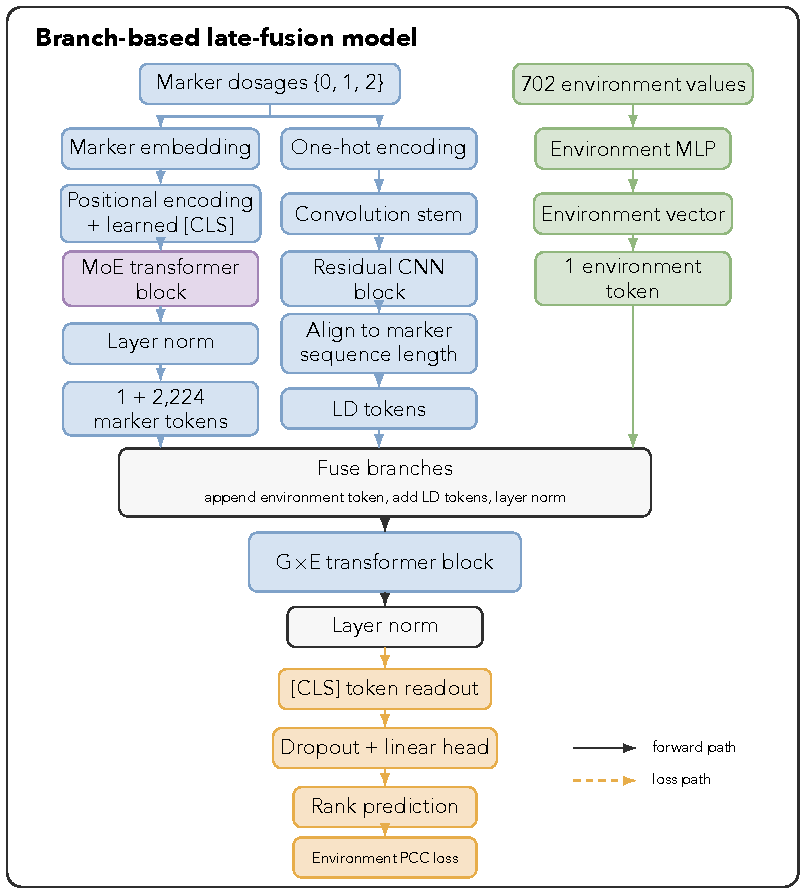
\includegraphics[width=0.78\linewidth]{figures/gxe-tf/branch-architecture.pdf}
    \caption{Branch-based late-fusion model used in the architecture comparison. Marker dosages enter a transformer encoder with a mixture-of-experts feed-forward layer and, in parallel, a one-hot convolutional encoder that captures local linkage-disequilibrium structure. The 702 environmental values enter a multilayer perceptron that produces a single environment token. The environment token is appended to the marker token sequence, the aligned LD representation is added elementwise, and a layer normalization combines them. One G$\times$E transformer block then processes the fused sequence, and a linear head reads the rank prediction from the \texttt{[CLS]} position. Blue blocks show marker operations, green blocks show environment operations, purple blocks show mixture-of-experts operations, and orange blocks show \texttt{[CLS]} and loss operations.}
    \label{fig:ch3-branch}
\end{figure}

The remaining two comparisons came from a later stage of development. Both used the environment-similarity auxiliary loss at weight $0.1$ and selected checkpoints on the macro environment PCC of the rank prediction. After comparing unified and branch-based architectures, we examined the effect of training objective choice. We trained two FullTransformer controls (Section~\ref{sec:ch3-architecture}) with identical architectures and principal hyperparameters, but optimized one model with the environment PCC loss defined in Section~\ref{sec:ch3-losses} and the other with a global MSE loss.

Finally, we compared the effect of the affine calibration head on absolute yield prediction. The reported FullTransformer used the environment PCC loss together with the affine calibration branch, while its control used the environment PCC loss alone. These two runs came from adjacent development commits, so this pair is near-matched rather than exactly matched.

Two runs of the environment PCC configuration completed at the same commit under identical settings. We report both and treat their difference as an estimate of run-to-run variation. Every other comparison arm is a single run, so this study does not yet estimate variation across random initializations. The complete experiment export contained 427 run records, of which 374 finished successfully. The accompanying machine-readable manifest records every exported run, its provenance, completion status, reported metrics, and manuscript disposition. Only completed comparisons from the legacy data scheme entered the primary results; experiments that used the later data-generation or tokenization schemes are designated as future work.

\section{Results}

\subsection{Performance on the 2024 Retrospective Benchmark}
On the 2024 retrospective benchmark, the reported affine-calibrated FullTransformer model achieved a macro environment PCC of $0.423$ and a macro environment MSE of $55.40$. These metrics came from the calibrated total prediction of the checkpoint selected by pre-2024 LEO validation. The result came from one run using seed 1, so no across-seed uncertainty estimate was available.

\subsection{Internal Model Comparisons}
We evaluated architectural and training variants during model development to determine how performance varied across design choices. Section~\ref{sec:ch3-comparisons} defines the three comparisons and the settings that differ between them. In the architecture comparison, the unified FullTransformer control achieved a macro environment PCC of $0.411$ and a macro environment MSE of $96.34$, whereas the branch-based late-fusion model achieved a macro environment PCC of $0.308$ and a macro environment MSE of $116.47$. These results indicate that unified processing of markers and environmental covariates was associated with better within-environment correlation and lower absolute error in this comparison.

Next, we examined how matching the primary training objective to the competition's evaluation metric affected performance. Both models were evaluated with macro environment PCC and macro environment MSE, although one optimized global MSE during training. The model trained with the environment PCC loss achieved a macro environment PCC of $0.423$ and a macro environment MSE of $100.57$. The model trained with the global MSE loss achieved a macro environment PCC of $0.305$ and a macro environment MSE of $14.54$. These results indicate that optimizing within-environment correlation substantially improved macro environment PCC but increased macro environment MSE, suggesting that the resulting predictions were less well-calibrated for absolute yield.

Motivated by this rank--scale trade-off, we compared a near-matched uncalibrated rank model with the reported affine-calibrated model. Both models achieved a macro environment PCC of $0.423$, but their macro environment MSE differed: $101.06$ for the uncalibrated model and $55.40$ for the affine-calibrated model. Calibration improved macro environment MSE by approximately $45.2\%$, while macro environment PCC changed by only $0.00004$. This behavior was expected because an environment-specific affine transformation with a positive scale preserves within-environment Pearson correlation while allowing the absolute scale and offset of the predictions to be adjusted.

The replicate pair described in Section~\ref{sec:ch3-comparisons} bounds how much of this variation is run-to-run noise. Its two runs agreed to three decimals on macro environment PCC at $0.423$, and gave macro environment MSE values of $100.57$ and $101.06$. These differences, $0.0000039$ in PCC and $0.50$ in MSE, provide the study's only estimate of run-to-run variation. On that scale, the $45.66$ MSE improvement from calibration is about 90 times the replicate difference. The corresponding PCC difference of $0.0000378$ amounts to $0.009\%$ of the score. Every other comparison arm is a single run. These results should therefore be interpreted as descriptive model-development comparisons rather than replicated estimates of individual-component effects. Table~\ref{tab:ch3-ablation-summary} reports the highlighted comparisons at full precision.

\begin{table}[htbp]
    \centering
    \footnotesize
    \begin{tabular}{@{}l l c c@{}}
        \toprule
        Comparison & Variant & \makecell{Macro environment \\ PCC} & \makecell{Macro environment \\ MSE} \\
        \midrule
        Architecture & Branch-based late-fusion model & 0.30819 & 116.46976 \\
                     & Unified FullTransformer control & 0.41066 & 96.33830 \\
        \addlinespace
        Training objective & Global MSE & 0.30504 & 14.54242 \\
                           & Environment PCC & 0.42316 & 100.56502 \\
        \addlinespace
        Calibration & Uncalibrated rank model & 0.42317 & 101.06046 \\
                    & Affine-calibrated model & 0.42321 & 55.40464 \\
        \bottomrule
    \end{tabular}
    \caption{Highlighted internal model-development comparisons on the retrospective 2024 benchmark. Comparisons should be made within, rather than across, the three labeled groups. Each row reports a single run. The architecture and objective pairs used matched principal settings; the calibration pair used near-matched runs from adjacent development commits. Values are given to five decimals so that the small differences discussed in the text remain visible. The complete run-level inventory is provided in \texttt{supplement/ablation\_run\_manifest.csv}.}
    \label{tab:ch3-ablation-summary}
\end{table}

\subsection{Performance Across Benchmark Environments}
To better understand the model's performance across environments, we examined variation in PCC among the 2024 benchmark environments (Figure~\ref{fig:ch3-environment-pcc}). All 22 environments in the benchmark cohort met the eligibility criteria described in the Evaluation section and yielded defined PCC values. Across these environments, the model achieved a mean PCC of $0.423$ and a median PCC of $0.434$. The interquartile range of environment-level PCC values was $0.364$--$0.480$, and the full range was $0.247$--$0.567$. The model achieved positive PCC in all 22 environments, with 16 of 22 ($72.7\%$) having PCC greater than $0.40$. Thus, performance was consistently positive but varied meaningfully among benchmark environments.

\begin{figure}[p]
    \centering
    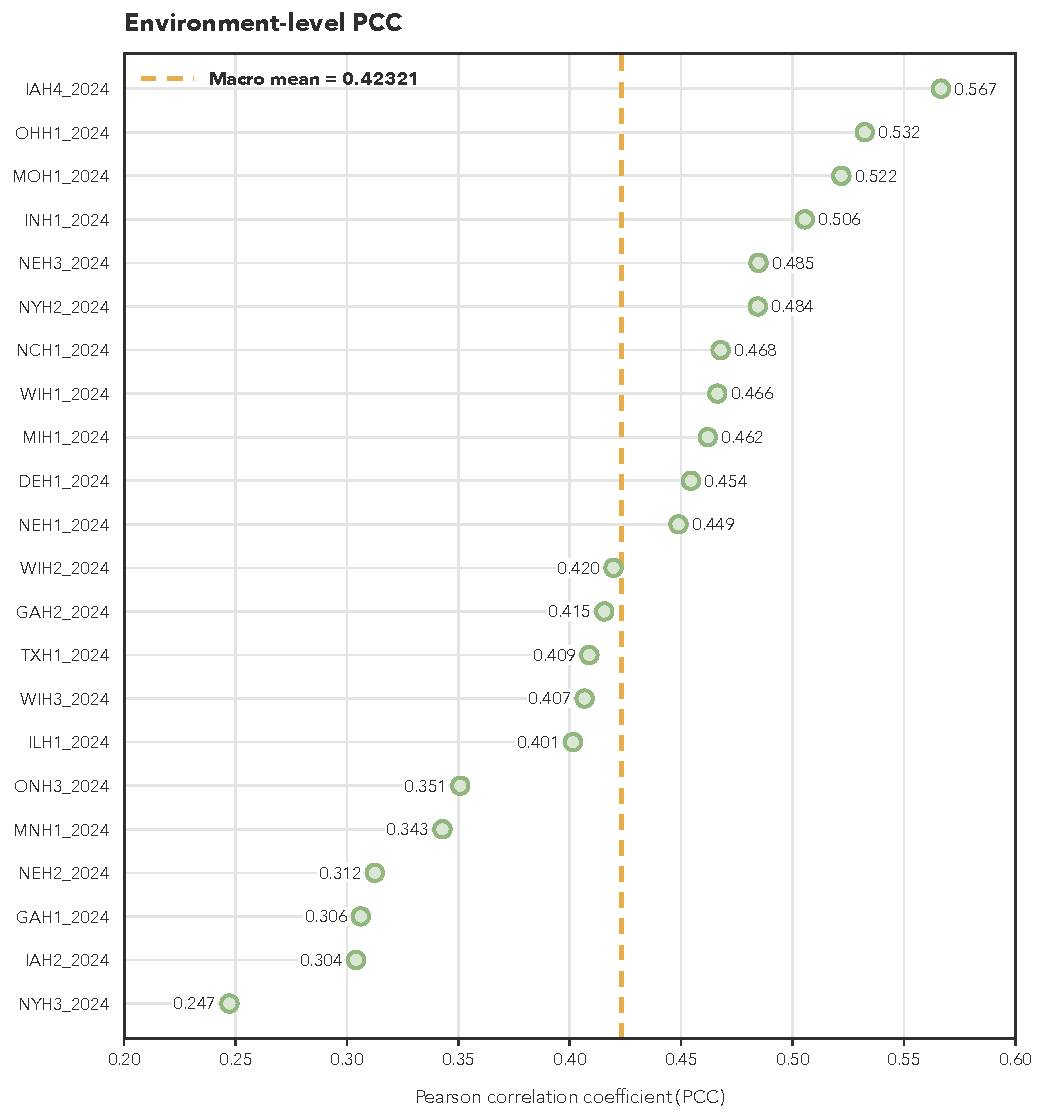
\includegraphics[width=\linewidth]{figures/gxe-tf/environment-level-pcc.pdf}
    \caption{Environment-level Pearson correlation coefficients (PCCs) for the selected FullTransformer checkpoint on the 2024 retrospective benchmark. Green points show PCC for each of the 22 environments in the benchmark cohort, ordered from highest to lowest. The dashed orange line marks the macro environment PCC of 0.423. Point labels show values rounded to three decimals.}
    \label{fig:ch3-environment-pcc}
\end{figure}

We also examined the upper and lower ends of the environment-level PCC distribution. The environment with the highest PCC was \texttt{IAH4\_2024}, with a PCC of $0.567$. The second-highest PCC occurred in \texttt{OHH1\_2024}, with a PCC of $0.532$, and the third-highest occurred in \texttt{MOH1\_2024}, with a PCC of $0.522$. In contrast, the environment with the lowest PCC was \texttt{NYH3\_2024}, with a PCC of $0.247$. The second-lowest was \texttt{IAH2\_2024}, with a PCC of $0.304$, and the third-lowest was \texttt{GAH1\_2024}, with a PCC of $0.306$. The difference between the highest and lowest environment-level PCC values was $0.319$, demonstrating considerable heterogeneity in model performance across environments.

\subsection{Competition Context} \comment{gotta make sure this is up-to-date with the new manuscript draft}
To contextualize the reported FullTransformer result, we compared it with the leading competing entries on the 2024 G2F G$\times$E Prediction Competition EvalAI leaderboard \cite{g2f-2024-evalai-leaderboard}. The competition ranked submissions using the macro environment PCC, the same primary metric used in our retrospective benchmark \cite{g2f-2024-competition}. Several leaderboard entries marked as \enquote{not competing} were omitted from this comparison \comment{update this: several entries were marked as not competing, and several were disqualified}. The FullTransformer achieved a PCC of $0.423$, which would have ranked third among the competing entries shown in Table~\ref{tab:ch3-external-results}. This score was $0.003$ lower than the fifth-place score and $0.027$ lower than the winning score. \comment{fix these numbers} Because the FullTransformer was evaluated after the competition and was not submitted, this placement is a retrospective comparison rather than an official result. Its proximity to the second-place score nevertheless indicates that the architecture was competitive with the leading competition entries.

\begin{table}[htbp]
    \centering
    \footnotesize
    \begin{tabularx}{\textwidth}{@{}c X c@{}}
        \toprule
        Rank & Entry & Competition PCC \\
        \midrule
        1 & Naaa & 0.45005 \\
        2 & NJUST\_KMG1 & 0.44402 \\
        3 & PARaBra & 0.43710 \\
        4 & transform(Base) & 0.42605 \\
        5 & The Cornquerors & 0.42574 \\
        (6) & FullTransformer (retrospective) & 0.42321 \\
        \bottomrule
    \end{tabularx}
    \caption{\comment{change the table to remove DQ'ed scores} Comparison of the FullTransformer result with the five leading competing entries on the 2024 G$\times$E Prediction Competition EvalAI leaderboard. Entries explicitly marked as not competing were omitted. The FullTransformer score is a retrospective comparison and was not an official competition submission; its rank is given in parentheses to mark the position the score would have taken.}
    \label{tab:ch3-external-results}
\end{table}


\section{Discussion}
This study tested whether a unified representation of marker and environmental tokens could support maize G$\times$E yield prediction more effectively than branch-based late fusion. Our results support early cross-modal interaction as a useful design choice and show that prediction rank and absolute scale require distinct treatment. The final FullTransformer combined these choices and achieved a competitive retrospective macro environment PCC of $0.423$ on the 2024 competition benchmark.

Unlike a late-fusion architecture, the FullTransformer places marker and environmental tokens in one sequence before either modality enters a separate encoder. This design gives each marker token a direct attention connection to every environmental token; thus, the model can form cross-modal representations before separate encoders can discard information needed for later interactions. Prior multimodal G$\times$E methods often use separate encoders and late fusion \cite{montesinos2024multimodal,shook2021crop}, so the comparison addresses a common design choice. The higher PCC and lower MSE of the unified control were consistent with this rationale. The unified model also reached the higher score with about half the trainable parameters of the branch-based late-fusion model, so capacity does not explain the difference. However, one seed and several component differences prevent a causal attribution to early fusion alone.

Objective choice exposed a practical trade-off between within-environment selection and absolute yield prediction. Macro environment PCC emphasizes whether the model preserves relative yield variation within each environment. By contrast, macro environment MSE penalizes errors in yield units, including errors in scale and offset. These metrics therefore support different uses: PCC supports hybrid selection within a trial, whereas MSE supports yield estimates on an absolute scale. The environment-conditioned affine head recovered part of the scale gap through a positive scale and shift that preserved within-environment PCC. In the near-matched comparison, this calibration reduced macro environment MSE by $45.2\%$, which supports separate correlation and scale targets. However, the calibrated model's macro environment MSE was still 3.8$\times$ higher than that of the global MSE-trained model. That model in turn reached a macro environment PCC of only $0.305$, $0.118$ below the calibrated model, so it would rank hybrids poorly within a trial. Calibration therefore narrowed the trade-off rather than removing it.

The mean benchmark PCC concealed substantial variation among the eligible 2024 environments. Although every environment had positive PCC, the model did not provide uniform reliability across environments. This variation could reflect differences in environmental complexity, data quality, sample composition, or other unmeasured factors, but this study did not test these explanations. These results show that model assessment requires both aggregate and environment-level metrics.

The retrospective placement below the two leading entries supports competitiveness, but it does not constitute an official competition result. Public leaderboard records do not describe each submission method, so score differences cannot identify which architecture choices caused the placement. The 2022 G2F competition also found no clear advantage for one model family \cite{g2f-maize-2025}. This broader pattern suggests that the FullTransformer score establishes method viability, not architecture superiority. \comment{can we use what we know in the unifinished manuscript?}

\subsection{Limitations and Future Work}
Each highlighted comparison used one seed, so the study could not estimate variation across random initialization. Future work should evaluate multiple seeds to quantify variation across model initializations.

The architecture comparison matched principal training settings, but its two designs differed in several components. The calibration comparison also used near-matched runs from adjacent commits. These comparisons therefore provide descriptive evidence rather than isolated causal effects. Future work should use controlled single-component ablations across multiple seeds.

The study used the 2024 labels for several model comparisons, so the benchmark was not an untouched external test set. The reported scores therefore describe retrospective benchmark performance, not a prospective competition submission. After method development, we will evaluate the FullTransformer on a future G2F season or another untouched benchmark.

Leave-environment-out validation holds out whole environments from the pre-2024 years, so it measures spatial interpolation for hybrids that the model has already seen. The 2024 benchmark posed a different problem. All 22 of its environments were new to the model, and $87.6\%$ of its hybrids were crosses absent from the training data. We therefore selected the reported checkpoint with a criterion that does not completely track benchmark performance. An improvement measured under leave-environment-out validation need not transfer to novel crosses in a novel year. Future work should build a validation design that reproduces the novel-cross and novel-year structure of the benchmark.

The tester composition of the benchmark was also highly asymmetric. PHP02 accounted for 5,119 of the 9,486 rows and LH287 for 3,716, which left 651 rows for all other testers. The reported scores therefore describe performance on crosses to two tester backgrounds. They provide little evidence about hybrids with other testers.

Access to compute constrained the design of the study. Training the reported model required 32 GPUs across four nodes of a shared supercomputer, and every run depended on an allocation award and on queue scheduling. This constraint, rather than the cost of any single run, is the practical reason the highlighted comparisons use single runs rather than replicated seeds. The reported result also rests on one checkpoint and its captured run configuration. We will archive that checkpoint, its configuration, the benchmark predictions, and the metric output with the manuscript.

In addition to the future work that is necessary to address the study's limitations, we outline several directions for further model improvement. First, we plan to evaluate the new reproducible data pipeline and feature tokenization options. The pipeline creates traceable and repeatable data from the raw competition files, including fixed imputation, filters, feature order, and data splits. This structure will also support controlled tests of alternative preprocessing choices. The tokenization options will support feature-aware representations for temperature, precipitation, soil, management, and other environmental covariates.

Furthermore, we plan to add temporal detail to the weather representation. The current model uses seasonal weather summaries, which can hide the date and crop stage of a weather event. Instead, we plan to test a weather encoder that can process daily weather sequences from planting to harvest. This approach will align weather features by days after planting rather than calendar dates. Development measures, such as growing degree days, could provide a closer link to crop stage. A transformer, RNN, or LSTM will convert the daily sequence into one or more weather tokens.

The model can then use attention to combine these tokens with soil, management, and marker tokens. We will compare seasonal weather summaries, temporal weather tokens, and their combination for G$\times$E prediction.

In addition to improving data and environmental representations, we plan to test whether external parental representations improve predictions for unseen hybrids. Currently, the model uses a shared learned dosage embedding across markers, with positional codes that identify loci. We plan to evaluate external parental information, such as parent genotypes, pedigree or relationship data, and known tester identity. Parent genotype data may overlap with hybrid marker data, but direct parental representations could expose inheritance and relationships more clearly.

We will compare hybrid markers alone with parent identity tokens, parent genotype representations, pedigree data, and combining-ability features. We will calculate any combining-ability features from the fit partition only to prevent target leakage. We will report performance on novel crosses, known crosses, and major testers.

Two further directions follow from the results reported above. The affine calibration head was trained as a low-weight auxiliary objective, so we will test whether a stronger calibration objective reduces macro environment MSE further without harming macro environment PCC. We will also test whether environmental complexity, data quality, or sample composition explain the variation in environment-level PCC, and whether environment-specific adaptation or calibrated uncertainty estimates improve reliability across environments.

All future comparisons will use multiple paired seeds and report mean scores, standard deviations, and paired differences to measure effects beyond seed variation.

    \chapter{MENTOR-RL}\label{ch:mentor-rl}

\section{Introduction and Motivation}

\subsection{Biological Interpretation as Mechanistic Discovery}
Biological interpretation involves the development and discovery of mechanistic relationships between biological entities such as genes, proteins, RNA, and other molecular components. Interpretation is essential for discovering context-specific relationships and developing models of disease, phenotypes, pathways, and regulatory systems. Recently, machine learning (ML) and artificial intelligence (AI) techniques such as iterative random forest (iRF)~\cite{basu2018iterative, cliff2019high} and related approaches have accelerated research through the construction of biologically informed networks, which scientists explore to generate mechanistic and functional hypotheses.

As these methods increase the resolution and scope of networks, biological interpretation has become increasingly mediated by large, multi-scale graph structures. To comprehensively examine these large biological networks and supporting databases, mechanistic exploration requires iterative querying and multi-step reasoning. Recent agentic interpretation systems such as eubiota~\cite{eubiota} and \textsc{Mentor-IA}~\cite{mentor-ia} demonstrate that provenance-preserving retrieval and tool-mediated synthesis can yield high-fidelity mechanistic narratives. However, these pipelines depend on frontier model inference and are not fully optimized as a trainable policy.

\subsection{Biological Interpretation is Bottlenecked by Human Cognition and Frontier Model Cost}
Although ML/AI methods such as \textsc{Mentor}~\cite{mentor} have refined mechanistic focus into groups of functionally related modules of genes, these modules can still be massive and intractable for individual researchers to systematically explore. Additionally, most research emphasizes a deep-but-narrow focus on a small subset of functionally related genes, which can overlook broader, yet biologically meaningful, network context, particularly in highly interactive systems such as living organisms. As biological networks grow in complexity, the combinatorial space of possible multi-hop interactions expands rapidly, while human interpretive capacity remains fixed.

While large language models (LLMs) can synthesize large volumes of information, frontier inference cost scales with exploration length and reasoning depth, limiting agentic deployment for long-horizon network traversal. This mismatch creates a scaling limit in biological mechanistic interpretation: rich relational structures can be computed, but downstream synthesis remains constrained by human bandwidth and model cost. Consequently, the speed, breadth, and contextual depth of mechanistic discovery are limited, particularly for complex traits, polygenic diseases, and multi-layer regulatory systems.

\subsection{AI-Guided Reasoning to Extend Mechanistic Interpretation Beyond Human Scale}
Open-source LLMs present an opportunity to aid scientists in mechanistic discovery tasks without being cost prohibitive. Recent developments in agent-based systems enable models to invoke deterministic tools with structured interfaces, substantially reducing hallucination and enabling provenance-preserving exploration. We propose \textsc{Mentor-RL}, a reasoning agent trained on biological ground truth and verifiable interaction objectives, enabling scalable mechanistic exploration without reliance on proprietary models.

By training a transformer-based agent with reinforcement learning across tool-use tasks and contextual levels of biological network data, we aim to produce a model that can traverse complex networks, synthesize \textit{multi-hop} mechanistic hypotheses, and integrate both local functional structure and global topological context. Leveraging open-source model offerings allows local deployment, with training costs amortized across many exploration sessions. Rather than replacing scientific judgment, \textsc{Mentor-RL} extends the interpretive bandwidth of researchers, enabling broader, faster, and more context-aware mechanistic discovery.

We make five contributions: 

\begin{enumerate}
    \item We formalize mechanistic graph exploration as a sequential decision process with a single policy operating in two modes: an actor that proposes reasoning and tool calls, and a verifier that updates a structured hypothesis and emits a continuation decision.

    \item We construct a dual-source module training corpus, comprising \textsc{Mentor}-derived dendrogram modules and RWR++ elbow-filtered random-walk-with-restart lines-of-evidence (RWR-LOE) modules, supporting four task cases: partial group completion, mechanism explanation, noisy group refinement, and recognition of no shared mechanism.

    \item We design a deterministic, schema-grounded reward system over structured state transitions, enabling reproducible scoring without proprietary judges at the step level during preference optimization and the trajectory level for policy gradient optimization.
    
    \item We propose a staged training pipeline, including warm-start SFT, DPO on shared-prefix trajectory branches, and GRPO for long-horizon exploration. We pair this with a curriculum that scales task difficulty, noise, and trajectory length.

    \item We will release the training environment, evaluation harness, and trained checkpoints, and we will benchmark against frontier and open models under both empirical and blind expert-preference evaluation.
\end{enumerate}

\section{Background and Related Work}
\subsection{Biological Networks and Mechanistic Ground Truth}
\subsubsection{Systems Biology and Mechanistic Discovery}
Systems biology examines biological function by studying interactions between molecular entities such as genes, proteins, and metabolites, rather than analyzing their individual properties~\cite{hartwell1999molecular, barabasi2004network}. A central goal is identifying \textit{modules}, or groups of functionally related entities, and characterizing the mechanisms that underlie their behavior. Because network interactions can span multiple scales and regulatory layers, modern systems biology relies on multiplex and multilayer network representations to capture context-specific relationships~\cite{barabasi2011network, ideker2012differential}. Module-level analysis has become a foundational tool for identifying disease mechanisms, prioritizing drug targets, and interpreting polygenic phenotypes~\cite{menche2015uncovering}, motivating the need for curated, mechanistic ground truth data against which computational methods can be developed and evaluated.

\subsubsection{Curated Interaction Maps}
Large-scale systems biology depends on curated molecular interaction databases that capture experimentally supported relationships at varying levels of resolution. Creating high-coverage, expert-annotated networks is crucial for enabling large-scale systems biology studies and encouraging mechanistic discovery.  BioGRID~\cite{oughtred2021biogrid} catalogs physical and genetic interactions across humans and model organisms from both low- and high-throughput studies. Reactome~\cite{reactome, gillespie2022reactome} provides manually curated, reaction-level pathway models for human biology. While both resources supply rich interaction evidence, neither organizes proteins into functional groups with verified co-membership. The CORUM database~\cite{giurgiu2019corum, tsitsiridis2023corum} fills this gap by curating experimentally verified mammalian protein complexes exclusively from low-throughput experiments. By providing verified group membership, curated interaction maps serve as a high confidence reference for mechanistic relationships. These resources, however, cover only a small, well-studied fraction of the interactome and are costly to extend, motivating computationally derived module structures that scale across the entire genome.

\subsubsection{Genome-Wide Module Discovery with MENTOR}
A complementary approach to curated databases is deriving mechanistic ground truth directly from network structure. \textsc{MENTOR} (Multiplex Embedding of Networks for Team-Based Omics Research)~\cite{mentor} computes random-walk-restart (RWR) embeddings for every gene across the layers of a multiplex, converts the embeddings into pairwise distances, and applies hierarchical clustering to produce a genome-wide dendrogram in which leaves are genes and internal nodes represent successively coarser functional groups. Selecting subtrees from this dendrogram yields a module whose granularity is controlled by the merge height at which the cut is taken, producing a nested family of modules that span the entire gene universe of the underlying network. Unlike curated databases, \textsc{Mentor} provides module structure at genome scale and for arbitrary multiplexes, including tissue- and context-specific networks, trading literature-based verification for broad coverage and mechanistic coherence.

\subsubsection{Gene-Centric Module Discovery with RWR-LOE}
While \textsc{Mentor} produces modules through top-down hierarchical clustering of the full gene universe, a complementary bottom-up approach derives modules for each individual gene. Applying RWR-LOE~\cite{kainer2025rwrtoolkit} to a single seed gene $g$ yields a ranked list of all other genes, ordered by propagation proximity to the seed. RWR-LOE walks the entire multiplex, treating each layer as an independent line of evidence, so that final rankings reflect the combined network structure rather than a single interaction type. Rather than imposing a fixed neighborhood size, RWR++ elbow filtering selects the cutoff at the bend in the score-versus-rank curve for each seed. Retaining the seed and all genes before this adaptive cutoff yields a gene-centric module $C^{\text{loe}}_g$, producing one module per gene in the network. RWR-LOE modules provide a complementary, bottom-up source of mechanistic ground truth compared to hierarchical \textsc{Mentor} modules.

\subsubsection{Network Construction and Exploration on Multiplexes}
Because biological systems comprise many complementary interaction modalities, integrating them without losing information motivated the development of the multiplex network formalism~\cite{mucha2010community, de2013mathematical}, which represents the same node set across multiple edge layers of differing types. Multiplex networks support propagation methods such as random walk with restart (RWR)~\cite{kohler2008walking, cowen2017network}, community detection methods, and learned graph models for tasks such as node classification, link prediction, and disease gene prioritization. In this proposal, these methods primarily motivate the graph operators available to the agent, while \textsc{Mentor} and RWR-LOE define the module targets used for training and evaluation.

\subsection{Tool-Using Language Models for Scientific Reasoning}
\subsubsection{Transformer Reasoning with Tool Use}
In addition to deep learning's growing utility for biological discovery, neural language models have shown promise for complex reasoning tasks, especially when grounded with tool use.~\cite{wei2022chain} demonstrated that prompting a model to show its reasoning steps before answering questions led to improved multi-step task performance in a few-shot setting, and~\cite{kojima2022large} extended this result to show its effectiveness in a zero-shot scenario. Furthermore, adding self-consistency mechanisms~\cite{wang2022self} and branched reasoning paths with lookahead and backtracking~\cite{yao2023tree} have enhanced model reasoning capabilities. 

Despite this progress in model reasoning, probabilistic decoding and training data cutoffs still leave language models prone to errors, including hallucination. In turn, equipping models with the ability to use external tools during training or inference provides a layer of deterministic verification and enables interaction with the outside world. Toolformer~\cite{schick2023toolformer} showed that self-supervised fine-tuning of tool calls yielded better performance with lower hallucination across several benchmarks, and Gorilla~\cite{patil2024gorilla} extended this paradigm to handle large API vocabularies with retrieval. ReAct~\cite{yao2022react} showed that combining reasoning techniques with tool-based actions improved complex reasoning performance, and PAL~\cite{gao2023pal} converted reasoning into programs, showing improved performance on computational tasks. These works demonstrate the power of combined reasoning and tool use for complex, multi-step problem solving, but their applications to scientific reasoning remain underexplored.

\subsubsection{Agentic Architectures with Verification}
While reasoning and tool use techniques improve task solving capability, they lack an inherent verification mechanism, which is crucial for making factual scientific claims. Several works have explored self-verification through various methods. Self-Refine~\cite{madaan2023selfrefine} and Reflexion~\cite{shinn2023reflexion} both define an iterative reflection loop without weight updates to improve answer quality. Self-Refine uses a single model to generate, critique, and refine its own output, while Reflexion utilizes sequential refinement, storing reflections in a persistent verbal memory. Self-RAG~\cite{asai2023selfrag} fine-tunes a language model to emit reflection tokens that govern when to retrieve passages and how to assess their relevance and support. Eubiota~\cite{eubiota} extends the self-verification process to multi-agent systems, using a dedicated verifier with separate weights to check the groundedness and factuality of other agent outputs. These approaches establish self-verification as a core component of agentic systems, but none combine a shared-weight actor-verifier paradigm with reinforcement learning over deterministic, structured state rewards, which we develop in Section~\ref{sec:methods}.

\subsubsection{Agentic Gene Set Interpretation}
LLM-based gene set interpretation has progressed from precomputed embeddings to fully agentic systems. GenePT~\cite{chen2025simple} employs GPT-4 to create gene-level and cell-level embeddings from natural language for use in downstream interpretation tasks. GeneAgent~\cite{wang2025geneagent} utilizes a multi-step GPT-4 pipeline with self-verification and retrieval from biological databases to provide a human-readable interpretation for experimentally derived gene lists. \textsc{Mentor-IA}~\cite{mentor-ia} extends this paradigm by creating separate agents for mechanistic interpretation subtasks, such as literature search, enrichment analysis, network analysis, and verification, unifying these outputs into a single mechanistic summary. Eubiota~\cite{eubiota} functions similarly to \textsc{Mentor-IA}, but with a focus on the human gut microbiome. The authors partially train a planning agent with GRPO while keeping proprietary model-powered subagents frozen. While these works share \textsc{Mentor-RL}'s agentic framing for mechanistic interpretation, none implements a fully trainable, end-to-end policy over verifiable rewards, which we introduce in Section~\ref{sec:methods}.

\subsection{Reinforcement Learning for Long-Horizon Tool-Use}
\subsubsection{Preference Optimization}
Christiano et al. introduced deep reinforcement learning from human feedback (RLHF)~\cite{christiano2017rlhf}, replacing hand-specified reward functions with a value model trained on pairwise human preferences. This framework was extended by InstructGPT~\cite{ouyang2022instructgpt}, which applied RLHF to align large language model outputs with human preferences. Direct preference optimization~\cite{dpo} built on this work by deriving a mathematically equivalent objective that operates directly on preference pairs, only using the policy and a reference while foregoing the reward model. Azar et al. unified RLHF and DPO under $\Psi$PO, a general preference optimization framework, and introduced IPO to address DPO's tendency to overfit when observed preferences are deterministic or near-deterministic~\cite{azar2024general}. Hong et al. proposed ORPO, a single-stage alternative that merges preference alignment and SFT via an odds-ratio penalty, removing the need for a separate alignment stage~\cite{hong2024orpo}. While these methods carry varying tradeoffs, we elect to train \textsc{Mentor-RL} with DPO because our deterministic runtime supports scalable preference pair generation and the resulting checkpoint serves as a preference-aligned reference policy in the GRPO stage.

\subsubsection{Policy Gradient and Group-Relative Methods}
While preference optimization aligns LLMs to pairwise judgments, policy gradient methods optimize directly against scalar rewards over rollouts, supporting online learning across a wide range of tasks. Proximal policy optimization (PPO)~\cite{schulman2017proximal} was introduced as a simple, efficient, and scalable alternative to TRPO~\cite{schulman2015trust}, using a clipped probability ratio term to form a pessimistic surrogate of performance, preventing excessively large policy updates. In RLHF~\cite{ouyang2022instructgpt}, this is paired with a token-wise KL penalty against a reference policy to anchor the model to its supervised initialization. Group relative policy optimization (GRPO)~\cite{shao2024deepseekmath} builds on PPO, computing the advantage term by measuring the deviation of outputs from a group mean rather than using a trained value model. Removing the critic network roughly halves the trainable parameters relative to PPO, making large-scale training more feasible. DeepSeek-R1~\cite{guo2025deepseek} demonstrated that GRPO with verifiable rewards can elicit emergent long-horizon reasoning behaviors at frontier scale. Having no learned critic, group-normalized advantages, and compatibility with deterministic verifiable rewards makes GRPO conducive to \textsc{Mentor-RL}, where the reward is a structured, schema-grounded signal over multi-hop biological graph exploration. 

\subsubsection{RL for Tool-Augmented Agents}
In addition to its usefulness for general LLM training, RL and adjacent post-training methods have been extensively used to train LLM agents in tool-use scenarios. WebGPT~\cite{nakano2021webgpt} used a fine-tuning, PPO, and rejection sampling pipeline to train a language agent for browser use and citation-backed question answering. ReST$^{EM}$~\cite{singh2023beyond} frames self-training from synthetic data as expectation maximization, demonstrating that fine-tuning on model-generated, filtered data can outperform fine-tuning on human-labeled datasets in verifiable reward settings. Toolformer~\cite{schick2023toolformer} demonstrated that LLMs can use external tools by sampling candidate API calls during pretraining and retaining those whose outputs reduce the loss on subsequent tokens. Building on this self-supervised paradigm, ToolLLM~\cite{qin2023toolllm} trained a language model for multi-step, multi-tool question answering on over 16,000 APIs with imitation learning. Agent-Q~\cite{putta2024agent} utilizes Monte Carlo tree search and process supervision to construct model trajectories, which are used to optimize an agent via DPO. These works provide methodological precedent for \textsc{Mentor-RL}; however, we utilize on-policy trajectory generation and deterministic rewards grounded in network-derived targets as a source of truth. 

\section{Proposed Methodology}\label{sec:methods}
Our methodology has five components. Sections~\ref{sec:agent_loop} and~\ref{sec:task} formalize the iterative exploration loop and the mechanistic interpretation task. Sections~\ref{sec:data} and~\ref{sec:trajectory} describe dataset construction and environment design. Sections~\ref{sec:rewards},~\ref{sec:training}, and~\ref{sec:curriculum} define the training pipeline, reward functions, and curriculum. Finally, Section~\ref{sec:eval} describes evaluation and benchmarking.

\subsection{Agent Loop Formulation}\label{sec:agent_loop}
\subsubsection{Loop Formalization}
We model mechanistic graph exploration as a sequential decision process executed by a single policy model with an internal self-verification step. The loop begins when the user provides a query, $q$, and optional evidence $e^{\text{user}}$, which may include text context, seed genes, or a multiplex network. These inputs initialize the working interpretation $I_0$ and the structured state $S_0$.

For each decision point $t < T_{\max}$, the current decision context is
\[
D_t = (q, e^{\text{user}}, I_t, S_t).
\]

Given $D_t$, the agent emits an action consisting of a textual reasoning step $r_t$ and an optional tool action $a_t$. The reasoning step specifies the current subgoal or interpretation update, while the tool action specifies a runtime-executable call. If a tool action is emitted, it is executed by a deterministic runtime $\varepsilon$; otherwise, the observation is empty.

After the action is produced and any deterministic tool calls are executed, the same policy enters a verification mode. Conditioned on the query, user-provided evidence, the current interpretation, the current structured state, and the current reasoning/action outputs, the verifier updates the interpretation and structured state, yielding $(I_{t+1}, S_{t+1})$. It also emits a continuation decision,
\[
z_t \in \{\texttt{continue}, \texttt{revise}, \texttt{stop}\},
\]
which determines whether the current interpretation should be extended, revised, or terminated. The decision \texttt{revise} indicates that the next iteration proceeds by correcting the interpretation and structured state rather than simply extending them.

The process repeats until either $z_t = \texttt{stop}$ or the maximum decision budget $T_{\max}$ is reached. At termination, $I_T$ and $S_T$ are returned as outputs. $I_T$ provides a human-readable answer to the query with respect to the accumulated evidence, while $S_T$ stores the corresponding verifiable outputs for reward computation and provenance preservation.

We formalize one iteration of the agent loop as
\[
r_t, a_t \sim \pi_{\theta}^{\mathrm{act}}(\cdot \mid D_t), \qquad
o_t = \varepsilon(a_t), \qquad
I_{t+1}, S_{t+1}, z_t \sim \pi_{\theta}^{\mathrm{verify}}(\cdot \mid r_t, a_t, o_t, D_t),
\]
where $r_t$ is the agent's textual reasoning or subgoal, $a_t$ is the optional tool action, and $o_t$ is the observation returned by the deterministic runtime $\varepsilon$, with $\varepsilon(\varnothing)=\varnothing$ by convention. The policies $\pi_{\theta}^{\mathrm{act}}$ and $\pi_{\theta}^{\mathrm{verify}}$ denote two prompting modes of the same underlying model, sharing weights so that biological vocabulary and tool-use competence learned in one mode transfers to the other. We treat the risk that the verifier collapses as a monitoring concern during training, discussed in Section~\ref{sec:limitations}. At each decision point, the pair $(I_t, S_t)$ represents the current mechanistic hypothesis, with $I_t$ serving as a human-readable view and $S_t$ as a machine-readable view of the same underlying state. The full agent loop algorithm is detailed in Algorithm~\ref{alg:agent-loop}.

\begin{algorithm}[t]
\caption{The \textsc{Mentor-RL} agent loop}
\label{alg:agent-loop}
\begin{algorithmic}[1]
\Require query $q$, user evidence $e^{\text{user}}$, maximum decision budget $T_{\max}$, deterministic runtime $\varepsilon$
\State Initialize working interpretation $I_0$ and structured state $S_0$ from $(q, e^{\text{user}})$
\State $T \gets 0$
\For{$t = 0, 1, \dots, T_{\max}-1$}
    \State $D_t \gets (q, e^{\text{user}}, I_t, S_t)$
    \State $(r_t, a_t) \sim \pi_{\theta}^{\mathrm{act}}(\cdot \mid D_t)$
    \If{$a_t \neq \varnothing$}
        \State $o_t \gets \varepsilon(a_t)$
    \Else
        \State $o_t \gets \varnothing$
    \EndIf
    \State $(I_{t+1}, S_{t+1}, z_t) \sim \pi_{\theta}^{\mathrm{verify}}(\cdot \mid r_t, a_t, o_t, D_t)$
    \State $T \gets t+1$
    \If{$z_t = \texttt{stop}$}
        \State \textbf{break}
    \EndIf
\EndFor
\State \Return final interpretation $I_T$ and structured state $S_T$
\end{algorithmic}
\end{algorithm}

\begin{figure}[htb!]
    \centering
    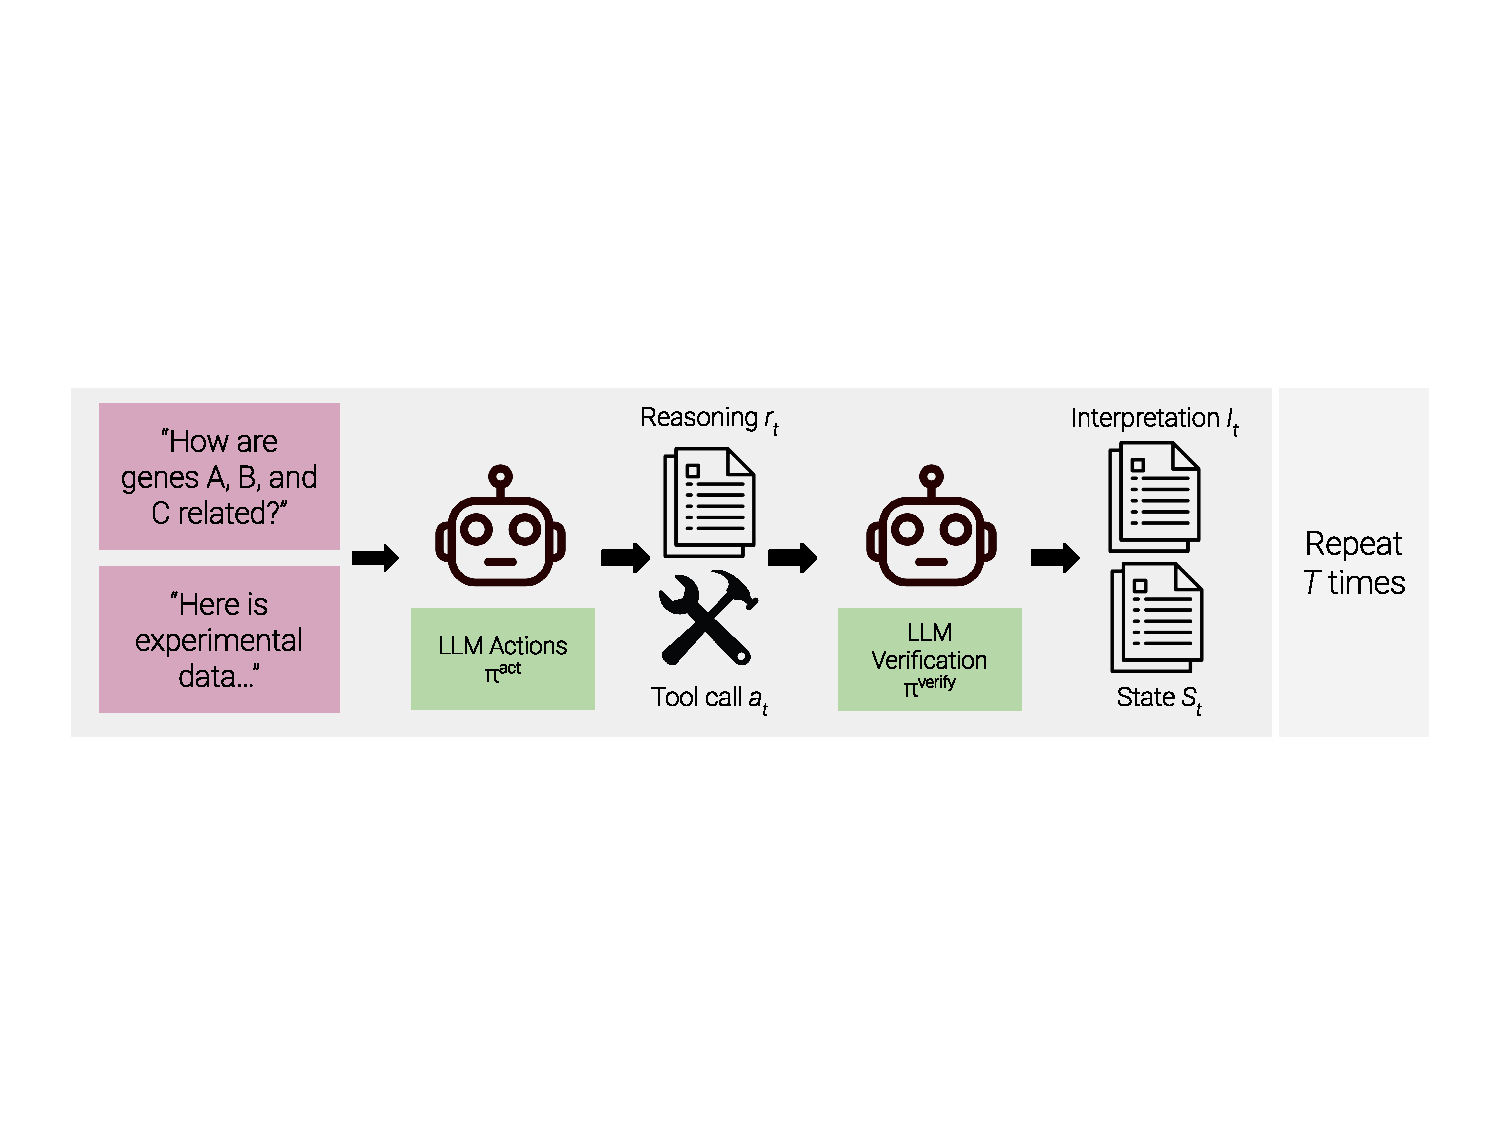
\includegraphics[width=\linewidth]{figures/mentor-rl/agent_loop.pdf}
    \caption{The \textsc{MENTOR-RL} agent loop.}
    \label{fig:agent-loop}
\end{figure}

\subsubsection{Working Interpretation}
The working interpretation $I_t$ is the human-readable form of the current mechanistic hypothesis and contains:
\begin{enumerate}
    \item the current mechanistic claim,
    \item the main evidence supporting that claim,
    \item any uncertainty, conflict, or alternative explanation,
    \item the next question or subgoal the model is trying to resolve.
\end{enumerate}

\subsubsection{Structured State}\label{sec:structured_state}
The structured state $S_t$ stores the same hypothesis in a machine-readable form suitable for tool execution, reward computation, and provenance tracking. It contains:
\begin{enumerate}
    \item the user-provided anchors $(q, e^{user})$,
    \item the current relationship status (unknown, partially observed group, validated group, multiple groups, or insufficient support) $(rel_t)$,
    \item the current predicted group or groups $(G_t)$,
    \item the evidence and provenance collected so far $(E_t)$,
    \item the current predicted mechanistic labels, each tied to the evidence handles that support it,
    \item the tool-use counters recording total and invalid tool calls $(n_{total}, n_{inv})$,
    \item the remaining budget and continuation state, and, at termination, the recorded termination signal $((T_{\max} - T), z_t)$.
\end{enumerate}

\subsection{Task Outputs and Mechanistic Targets}\label{sec:task}

\subsubsection{Final Interpretation}
The final outputs of the model are the terminal interpretation $I_T$ and the terminal structured state $S_T$. Together, these outputs must support four cases: completion of a partially observed mechanistic group, explanation of an already coherent group, refinement of a noisy group, and recognition that no single shared mechanism is supported. The final interpretation states which case is supported by the evidence, summarizes the main evidence for that claim, and links the evidence to the claim through reasoning traces and tool calls. It also records uncertainty or abstention when evidence is incomplete. If the loop terminates with $z_t = \texttt{stop}$, the next subgoal field is left blank. If the loop terminates because the decision budget $T_{\max}$ is exhausted, the interpretation may include a recommended next subgoal to guide further exploration.

\subsubsection{Final Structured State}
The final structured state is a schema-enforced JSON object. It contains the same components defined in Section~\ref{sec:structured_state}, but with finalized values for relationship status, predicted groups, collected evidence, and mechanistic labels. These values are used for reward evaluation and provenance tracking. The final structured state also records whether termination occurred because the model emitted $z_t = \texttt{stop}$ or because the budget $T_{\max}$ was exhausted. If the budget is exhausted, the remaining budget is $0$; if the model stops early, the remaining budget is $T_{\max} - T$.

\subsubsection{Supported Task Cases}
We support four output cases during training to reflect the variability of experimental evidence that users may provide:
\begin{enumerate}
    \item partial group completion,
    \item mechanism explanation for an already related group,
    \item group refinement from a noisy module,
    \item no single shared mechanism.
\end{enumerate}

Partial group completion occurs when the user provides a subset of related genes; the model expands this subset into a larger mechanistically related group and explains it. Mechanism explanation occurs when the user provides a complete module; the model explains the mechanism without unnecessary expansion. Group refinement occurs when the user provides a known module with several unrelated noise genes; the agent refines the group so that it contains only mechanistically related genes. Finally, in the no shared mechanism case, the user provides genes that do not support one coherent mechanism, and the model either splits them into multiple groups or returns insufficient support.

\subsubsection{Targets for Training and Evaluation}
We define two complementary target types for training and evaluation. \textbf{Module membership targets} are the hidden gene sets drawn from either \textsc{Mentor}-derived dendrogram modules or elbow-filtered RWR-LOE modules (Sections~\ref{sec:mentor-corpus} and~\ref{sec:loe-corpus}). These targets are only used for scoring: the agent never observes hidden module members and must recover them through exploration. These modules supply the supervised signal for set-level recovery, refinement, and abstention.

Because dendrogram modules are derived computationally from multiplex structure, they offer genome-wide coverage, but often without per-entry experimental annotations. \textbf{Mechanistic evidence targets} therefore score the quality of a final explanation against the evidence retrieved during exploration, such as enrichment, annotation, and graph support. This allows interpretations to be rewarded for being grounded in evidence rather than simply matching a pre-defined annotation, which encourages the exploration of novel biology beyond existing databases.

\subsection{Data, Resources, and Environment}\label{sec:data}
Our dataset is constructed from a combination of existing internal tool infrastructure, open-source biological resources, and graph exploration environments.

\subsubsection{Warm-Start SFT Dataset} 
We first construct a warm-start SFT subset from the \textsc{Mentor-IA} tool stack~\cite{mentor-ia}, including gene metadata, gene ontology (GO) annotations, pathway membership, and literature evidence. These data are retrieved via MyGene.info~\cite{mygene.info} and Europe PMC~\cite{europepmc}. This warm-start subset covers four task families:
\begin{enumerate}
    \item entity normalization, such as resolving gene names and synonyms to canonical identifiers,
    \item annotation retrieval, such as returning GO terms, localization, and pathway information for a gene or gene set,
    \item literature-grounded extraction, such as identifying relevant genes, pathways, or mechanisms from retrieved abstracts, and
    \item evidence-to-finding generation, which converts retrieved tool outputs into short, grounded mechanistic statements.
\end{enumerate}

We include tool-enabled (open-book) and tool-disabled (closed-book) questions, with open-book examples emphasized to promote schema-valid tool use and evidence grounding, and closed-book examples used to strengthen biological vocabulary and lightweight recall. To make this stage reproducible, API responses and database versions will be cached during dataset construction.

To make the warm-start SFT stage concrete, we define a core tool vocabulary derived from the existing \textsc{Mentor-IA} infrastructure~\cite{mentor-ia} in Table~\ref{tbl:tools}. Early SFT emphasizes schema-valid biological annotation and enrichment calls, while graph-exploration and RWR++ operators are introduced during DPO and online RL.

\begin{table}[p]
\centering
\caption{Tool vocabulary for the \textsc{Mentor-RL} agent. Related RWR++ calls are grouped by function while preserving the model-facing tool names.}
\label{tbl:tools}
\scriptsize
\setlength{\tabcolsep}{3pt}
\renewcommand{\arraystretch}{0.95}
\begin{tabularx}{\textwidth}{@{}>{\raggedright\arraybackslash}p{0.34\textwidth} >{\raggedright\arraybackslash}X >{\raggedright\arraybackslash}p{0.25\textwidth} >{\raggedright\arraybackslash}p{0.08\textwidth}@{}}
\toprule
\textbf{Tool(s)} & \textbf{Purpose} & \textbf{Primary inputs} & \textbf{Stage} \\
\midrule
\texttt{query\_mygene} & Gene metadata, GO terms, pathways, and summaries & \texttt{query}; requested \texttt{fields} & SFT \\
\midrule
\texttt{enrich\_gene\_set} & Functional enrichment over a candidate gene set & \texttt{genes}; \texttt{background}; \texttt{top\_k}; threshold & SFT, DPO, RL \\
\midrule
\texttt{get\_neighbors}; \texttt{induce\_subgraph} & Local native graph and induced-subgraph evidence & gene or gene-set identifiers; layers & DPO, RL \\
\midrule
\texttt{rwr}; \texttt{rwr\_loe}; \texttt{shortest\_paths} & RWR++ expansion, leave-one-out relatedness, and path evidence & seed, query, source, or target genes; layers; \texttt{top\_k} & DPO, RL \\
\midrule
\texttt{get\_rank}; \texttt{get\_distance}; \texttt{get\_spearman}; \texttt{get\_pearson}; \texttt{get\_dot\_similarity} & Rank, distance, and vector-similarity comparisons & paired genes; metric; layers & DPO, RL \\
\midrule
\texttt{get\_rank\_vector\_summary}; \texttt{get\_encoding\_summary} & Compact rank-vector and encoding summaries & seed or query genes; layers; \texttt{top\_k} & DPO, RL \\
\midrule
\texttt{get\_gene\_layers}; \texttt{get\_nodes\_by\_layer}; \texttt{get\_layer\_stats}; \texttt{get\_path\_layer\_counts}; \texttt{get\_component\_summary} & Layer membership, layer statistics, path support, and components & genes or layers, depending on query & DPO, RL \\
\midrule
\texttt{get\_seed\_essentiality}; \texttt{get\_layer\_ablation}; \texttt{get\_node\_perturbation} & Stability, ablation, and perturbation analyses & seed or perturbation genes; layers; \texttt{top\_k} & DPO, RL \\
\bottomrule
\end{tabularx}
\end{table}

\subsubsection{\textsc{Mentor}-Derived Training Corpus}\label{sec:mentor-corpus}After constructing the warm-start SFT dataset, we create two complementary module corpora that together supply the hidden targets for trajectory generation: a \textsc{Mentor}-derived corpus (this section) and an RWR-LOE corpus (Section~\ref{sec:loe-corpus}). We first parse the genome-wide \textsc{Mentor} dendrogram into modules, where each module is the gene set of a dendrogram subtree. We partition the modules into train, validation, and test splits to prevent leakage across stages.

For each module $C_{\text{module}}$ of size $n$, we deterministically materialize up to four task instances, one per case in Section~\ref{sec:task}. This ensures that all four task types are represented for as many modules as possible rather than sampled independently. The \texttt{explanation} instance uses the full module as input, $C^{\text{in}} = C_{\text{module}}$. The \texttt{recovery} instance drops $k_{\text{drop}}$ genes from the module, $C^{\text{in}} = C_{\text{module}} \setminus G_{\text{drop}}$, and the \texttt{refinement} instance adds $k_{\text{add}}$ noise genes, $C^{\text{in}} = C_{\text{module}} \cup G_{\text{add}}$. In both the recovery and refinement cases, the hidden target remains $C = C_{\text{module}}$. The number of genes added or dropped scales with the task difficulty and module size, so that harder instances perturb a larger fraction of the module. The \texttt{none} instance constructs a pseudo-module of unrelated genes as input with hidden target $C = \varnothing$.

Noise and \texttt{none} genes are drawn from difficulty-modulated \textit{dendrogram distance bands}, which are defined by walking up the module's ancestry in the tree, so that difficulty controls how topologically close the distractors are to the module. Additionally, \texttt{none} genes are constrained to be conflict-free (i.e. they are not related to each other), so that sampled genes do not form a coherent module themselves. All selection is deterministic given a fixed seed, making the corpus reproducible. The resulting \textsc{Mentor}-based corpus provides supervision for schema-valid tool use and for the terminal outputs of Section~\ref{sec:task}.

\begin{algorithm}[t]
\caption{Creation of the \textsc{Mentor}-derived module training corpus}
\label{alg:mentor-module-corpus}
\begin{algorithmic}[1]
\Require dendrogram $D$, multiplex $M$, difficulty map $\delta$

% initialize modules from the dendro, parsing into train/val/test splits
\State Parse the genome-wide \textsc{Mentor} dendrogram $D$ over multiplex $M$ into modules $\{C_{\text{module}}\}$
\State Partition modules into train/validation/test splits at the module level

% loop through each module and create task instances for each case w/ set difficulty and size
\For{each module $C_{\text{module}}$ in split with difficulty map $\delta$}
    \State $n \gets |C_{\text{module}}|$

    \State \textbf{// explanation}
    \State emit $(C^{\text{in}} = C_{\text{module}},\; C = C_{\text{module}},\; \texttt{explanation},\; rel=\texttt{validated\_group})$

    \State \textbf{// recovery}
    \State $k_{\text{drop}} \gets \textsc{DropCount}(n, \delta_{\text{rec}})$;\quad $G_{\text{drop}} \gets \textsc{DetSelect}(C_{\text{module}}, k_{\text{drop}})$
    \State emit $(C^{\text{in}} = C_{\text{module}} \setminus G_{\text{drop}},\; C = C_{\text{module}},\; \texttt{recovery},\; rel=\texttt{validated\_group})$

    \State \textbf{// refinement}
    \State $k_{\text{add}} \gets \textsc{NoiseCount}(n, \delta_{\text{ref}})$;\quad $G_{\text{add}} \gets \textsc{DendroNeg}(C_{\text{module}}, k_{\text{add}}, \delta_{\text{ref}})$
    \State emit $(C^{\text{in}} = C_{\text{module}} \cup G_{\text{add}},\; C = C_{\text{module}},\; \texttt{refinement},\; rel=\texttt{validated\_group})$

    \State \textbf{// none}
    \State $G_{\text{none}} \gets \textsc{DendroNeg}(C_{\text{module}}, n, \delta_{\text{none}},\, \text{conflict\_free})$
    \State emit $(C^{\text{in}} = G_{\text{none}},\; C = \varnothing,\; \texttt{none},\; rel=\texttt{insufficient\_support})$
\EndFor
\State \Return all task instances
\end{algorithmic}
\end{algorithm}

\subsubsection{RWR-LOE Module Corpus}\label{sec:loe-corpus}
In addition to the top-down, hierarchical \textsc{Mentor}-derived module corpus, we create a corpus of RWR-LOE exploration across all genes in the multiplex to provide a bottom-up complement. For each gene $g$ in the same multiplex universe as the \textsc{Mentor} dendrogram, we run \texttt{rwr\_loe}$(g)$ to obtain a propagation score and rank for every other gene in the network. We then apply the RWR++ elbow filter to the score-versus-rank curve for that seed, yielding an adaptive cutoff rank $r^\star_g$. The LOE module is defined as $C^{\text{loe}}_g = \{g\} \cup \{v : \mathrm{rank}_g(v) \le r^\star_g\}$, producing a single seed-specific module per gene without imposing a fixed module size.

For each module, we materialize the same four task instances as the \textsc{Mentor}-derived corpus. For difficulty control, we substitute RWR-LOE rank bands for dendrogram distance bands: noise and \texttt{none} genes are drawn from ranks just beyond, moderately beyond, or far beyond the seed's elbow cutoff. We partition RWR-LOE modules into train, validation, and test splits independently of the \textsc{Mentor}-derived modules, and module-size bins are assigned after construction from the realized values of $|C^{\text{loe}}_g|$. The two corpora are complementary: \textsc{Mentor} modules capture top-down, hierarchical functional organization, while RWR-LOE modules reflect bottom-up, seed-centered topology.
\begin{algorithm}[t]
\caption{Creation of the RWR-LOE module training corpus}
\label{alg:loe-module-corpus}
\begin{algorithmic}[1]
\Require multiplex $M$, gene universe $\mathcal{G}$, elbow-filter parameters $\phi$, difficulty map $\delta$
\State Partition $\mathcal{G}$ into train/validation/test splits at the gene level
\For{each gene $g \in \mathcal{G}$}
    \State Run $\texttt{rwr\_loe}(g, M)$ to obtain scores $s_g$ and ranked list $L_g$
    \State $r^\star_g \gets \textsc{ElbowCutoff}(L_g, s_g, \phi)$
    \State $E_g \gets \{v \in L_g : \mathrm{rank}_g(v) \le r^\star_g\}$
    \State $C^{\text{loe}}_g \gets \{g\} \cup E_g$,
           \quad $n \gets |C^{\text{loe}}_g|$
    \State \textbf{// explanation}
    \State emit $(C^{\text{in}} = C^{\text{loe}}_g,\; C = C^{\text{loe}}_g,\;
           \texttt{explanation},\; rel=\texttt{validated\_group})$

    \State \textbf{// recovery}
    \State $k_{\text{drop}} \gets \textsc{DropCount}(n, \delta_{\text{rec}})$;
           \quad $G_{\text{drop}} \gets \textsc{DetSelect}(C^{\text{loe}}_g,
           k_{\text{drop}})$
    \State emit $(C^{\text{in}} = C^{\text{loe}}_g \setminus G_{\text{drop}},\;
           C = C^{\text{loe}}_g,\; \texttt{recovery},\;
           rel=\texttt{validated\_group})$

    \State \textbf{// refinement}
    \State $k_{\text{add}} \gets \textsc{NoiseCount}(n, \delta_{\text{ref}})$;
           \quad $G_{\text{add}} \gets \textsc{RankBandNeg}(L_g, r^\star_g, k_{\text{add}},
           \delta_{\text{ref}})$
    \State emit $(C^{\text{in}} = C^{\text{loe}}_g \cup G_{\text{add}},\;
           C = C^{\text{loe}}_g,\; \texttt{refinement},\;
           rel=\texttt{validated\_group})$

    \State \textbf{// none}
    \State $G_{\text{none}} \gets \textsc{RankBandNeg}(L_g, r^\star_g, n, \delta_{\text{none}},
           \text{conflict\_free})$
    \State emit $(C^{\text{in}} = G_{\text{none}},\; C = \varnothing,\;
           \texttt{none},\; rel=\texttt{insufficient\_support})$
\EndFor
\State \Return all task instances
\end{algorithmic}
\end{algorithm}


\subsubsection{Graph Environment and Runtime}\label{sec:graph-runtime}
Each task instance is paired with a graph environment defined over the same canonical gene universe as the in-house brain multiplex, from which our module corpora are derived. The sampled input set $C^{\text{in}}$ initializes the agent's graph anchors, while the hidden target $C$ defines the supervisory signal.

To interface the graph environment with the training pipeline, we use a compiled native multiplex library exposed to Python through \texttt{ctypes} bindings~\cite{cpp}. Training, rollout, and optimization code are implemented in Python~\cite{python}, while graph storage and graph operations are handled by the native runtime for efficient execution on large multiplexes. Multiplex networks are persisted as raw, CSR-style binary stores described by JSON manifests; all graph input and output is binary, with the manifest carrying the layer names, node, and build metadata needed to load the graph.

The runtime uses a set of optimized multiplex functions developed as part of the \textsc{Mentor}~\cite{mentor} and \textsc{Mentor-IA}~\cite{mentor-ia} projects known as RWR++. Core operators include neighborhood retrieval, shortest-path search, random walk with restart on both monoplex and multiplex views, and subgraph induction. These operators provide the primary graph-facing actions available to the agent during exploration.

All runtime operators return both graph objects and provenance metadata. In addition to nodes, edges, and scores, each returned object records the relevant layer identity, operator parameters, and source information needed to trace the final interpretation back to the graph evidence used to construct it. To ensure consistency across serialized multiplex files, C++ runtime objects, Python wrappers, and logged training artifacts, all nodes are represented in a single canonical identifier space and all edges are referenced using deterministic, layer-aware identifiers.

\subsection{Trajectory Generation, Preference Mining, and Mechanistic Summary Construction}\label{sec:trajectory}

\subsubsection{Overview}
Using the module corpora and deterministic runtime defined in Sections~\ref{sec:mentor-corpus},~\ref{sec:loe-corpus}, and~\ref{sec:graph-runtime}, we generate shared-prefix trajectories for SFT and DPO. For each sampled task, the warm-start policy proposes multiple candidate next steps, deterministic execution produces candidate observations and next states. We employ structured branch scoring functions to rank these candidates, and the resulting rankings are converted into shared-prefix preference pairs. One branch per step is retained as the continuation of the logged trajectory, from which we derive per-step findings and a final mechanistic summary. The trajectory generation process is outlined in Algorithm~\ref{alg:trajectory-gen}.

\begin{algorithm}
\caption{Trajectory Generation for SFT and DPO}\label{alg:trajectory-gen}
\begin{algorithmic}
    % require policy, runtime, and hyperparameters
    \Require $\pi^{act}_\theta, \pi^{verify}_\theta$, runtime $\varepsilon$, $T_{\max}, n_{act}, n_{ver}, n_{cov}$, directives $\{d_i\}$, pair margin $\tau$, selection tolerance $\epsilon$.

    % sample a module task and evidence mode from the precomputed corpus
    \State Sample module task $(C^\text{in}, C, C_\text{type})$ and evidence mode $\rho$.
    \State $q, e^\text{user} \sim Q_\text{templates}(\cdot \mid C^\text{in}, C, C_\text{type}, \rho)$.
    
    % 0-init the interp and structured state along with trajectory, pref, and findings 
    \State $(I_0, S_0) \gets \mathrm{InitState}(q, e^\text{user}, C^\text{in})$.
    \State $\tau^\star \gets [\ ]$, \quad $\mathcal{P} \gets [\ ]$, \quad $\mathcal{F} \gets [\ ]$, \quad $T \gets 0$
    
    \State $z_{-1} \gets \texttt{continue}$

    % begin traj loop
    \For{$t = 0, 1, \dots, T_{\max} - 1$}
        % check for stop case (budget/continuation)
        \If{$z_{t-1} = \texttt{stop}$ \textbf{or} $\mathrm{budget}(S_t) \le 0$} \textbf{break} \EndIf
        
        % init decision context
        \State $D_t \gets (q, e^{user}, I_t, S_t)$, \quad $\mathcal{C}_t \gets [\ ]$, \quad $\mathcal{A} \gets [\ ]$
        
        % sample candidate actions and reasoning
        \For{$i = 0, \dots, n_{act}-1$}
            \State $(r_{t,i}, a_{t,i}) \sim \pi^{act}_\theta(\cdot \mid D_t, d_i)$; \quad append to $\mathcal{A}$
        \EndFor
        
        % if tool call fails, retry with tool-coverage directive  
        \If{$C_\text{type} \in \{\texttt{recovery}, \texttt{refinement}\}$ \textbf{and} no $a \in \mathcal{A}$ is a tool call}
            \For{$i = 0, \dots, n_{cov}-1$}
                \State $(r, a) \sim \pi^{act}_\theta(\cdot \mid D_t, d^{\text{cov}}_i)$; \quad append to $\mathcal{A}$
            \EndFor
        \EndIf

        % execute tool calls, apply verifier policy, update interp/state, and then score branches
        \For{each $(r_{t,i}, a_{t,i}) \in \mathcal{A}$}
            \State $o_{t,i} \gets \varepsilon(a_{t,i})$ if $\mathrm{ValidTool}(a_{t,i}, S_t)$ else $\varnothing$
            \For{$j = 0, \dots, n_{ver}-1$}
               \State $(I'_{t,i,j}, S'_{t,i,j}, z'_{t,i,j}) \sim \pi^{verify}_\theta(\cdot \mid D_t, r_{t,i}, a_{t,i}, o_{t,i})$
               \State $s^{local}_{t,i,j} \gets \mathrm{LocalScore}(D_t, I'_{t,i,j}, S'_{t,i,j}, r_{t,i}, a_{t,i}, o_{t,i}, z'_{t,i,j}; C, C_{\text{type}})$
               \State Append $c_{t,i,j}$ to $\mathcal{C}_t$
            \EndFor
        \EndFor

        % normalize scores, select branch, make preference pair for this iteration, update trajectory and findings, and update interp/state
        \State $\mathrm{NormalizeScores}(\mathcal{C}_t)$
        \State $(i^\star, j^\star) \gets \mathrm{SelectBranch}(\mathcal{C}_t; \epsilon)$
        \State $\mathcal{P} \gets \mathcal{P} \cup \mathrm{MakePreferencePairs}(\mathcal{C}_t, c_{t,i^\star,j^\star}, \tau)$
        \State Append $(I_t, S_t, c_{t,i^\star,j^\star})$ to $\tau^\star$; \quad $f_t \gets \mathrm{RenderFinding}(\cdot)$; append $f_t$ to $\mathcal{F}$
        \State $(I_{t+1}, S_{t+1}) \gets (I'_{t,i^\star,j^\star}, S'_{t,i^\star,j^\star})$; \quad $T \gets t+1$
    \EndFor
    % render final mech summary, return trajectory, prefs, findings, and summary
    \State $m \gets \mathrm{RenderSummary}(S_T, \mathcal{F})$
    \State \Return $\tau^\star, \mathcal{F}, m, \mathcal{P}$
\end{algorithmic}
\end{algorithm}

\subsubsection{Shared-prefix Trajectory Synthesis}\label{sec:shared-prefix}
Given a sampled task and initialized state, we sample multiple action candidates $(r_{t,i}, a_{t,i})$ given the current decision context $D_t$ and execute valid tool calls in the deterministic graph runtime. To ensure that candidates with the same prefix explore genuinely distinct regions of the action space, we use verbalized sampling based on the task type. For example, recovery prompts bias candidates towards random-walk expansion, neighborhood expansion, subgraph validation, or a direct decision, while insufficient evidence (\texttt{none}) prompts direct the model towards disconfirming graph evidence. When a sampling round for recovery or refinement tasks fails to produce valid tool calls, we issue a tool-coverage retry that requires a valid graph operator whenever one can be formed, which prevents the branch pool from degenerating into tool-free continuations. Conditioned on each candidate action and observation, the same policy then samples multiple verification candidates, yielding a tree of candidate next states rooted at a shared prefix. The branched sampling scheme is visualized in Figure~\ref{fig:shared-prefix}.

\begin{figure}[h!]
    \centering
    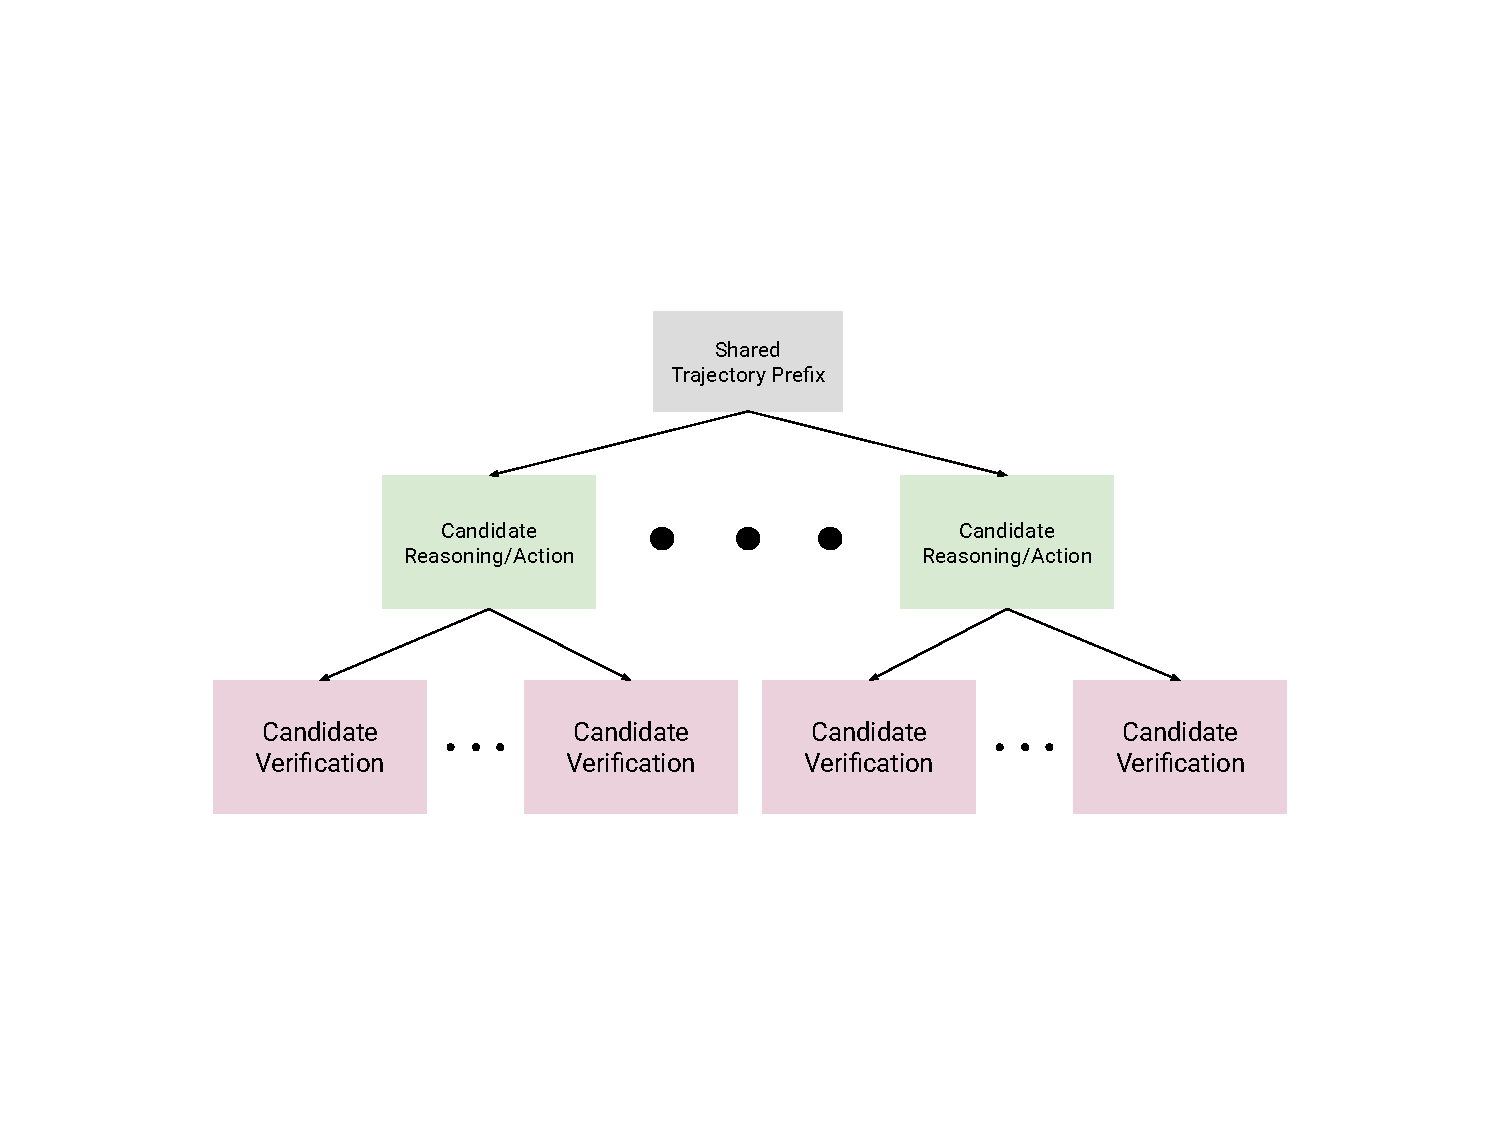
\includegraphics[width=\linewidth]{figures/mentor-rl/trajectory_gen.pdf}
    \caption{The shared prefix generation tree.}
    \label{fig:shared-prefix}
\end{figure} 

\subsubsection{Initialization, Tool Validation, and Query Construction}\label{sec:init-valid-query}

We define $\text{InitState}(q, e^{\text{user}}, C^{\text{in}})$ as a deterministic function that constructs the initial interpretation $I_0$ and structured state $S_0$ from the query, user-provided evidence, and seed gene set. The working interpretation $I_0$ is populated from a fixed template: the mechanistic claim is empty, the evidence field records only the user-provided inputs, the uncertainty field is blank, and the next subgoal is set to the query $q$. The structured state $S_0$ is initialized as follows:
\begin{enumerate}
    \item the user-provided anchors are set to $(q, e^{\text{user}})$,
    \item the relationship status $rel_0$ is set to \texttt{unknown},
    \item the predicted group is initialized to $G_0 = C^{\text{in}}$,
    \item the evidence log $E_0$ is empty,
    \item the predicted mechanistic labels are empty,
    \item the remaining budget is $T_{\max}$ and the continuation state is $z_0 = \texttt{continue}$.
\end{enumerate}
The agent does not observe the task type $C_{\text{type}}$, the true relationship status, or the hidden target $C$; it must infer the appropriate task case through exploration.

We define $\text{ValidTool}(a_{t,i}, S_t)$ as a deterministic function that checks whether a proposed tool action $a_{t,i}$ is executable given the current structured state $S_t$. Validation proceeds in two stages. First, the syntax check verifies that the tool name referenced in $a_{t,i}$ exists in the current tool vocabulary and that all arguments conform to the tool's input schema. Second, the semantic check verifies that basic conditions are satisfied with respect to the graph environment. For example, the function ensures that queried genes exist in the multiplex, requested layers are valid, and required fields in $S_t$ are populated. If either check fails, $\text{ValidTool}$ returns false and the observation $o_{t,i}$ is set to $\varnothing$. Invalid tool calls are counted toward $n_{inv}$ in the efficiency penalty (Equation~\ref{eqn:eff-pen}).

At inference time, users provide a natural language query $q$ alongside optional evidence $e^{\text{user}}$. Queries are unconstrained and may range from broad exploratory requests to specific hypothesis-driven questions. Evidence may include any combination of:
\begin{enumerate}
    \item a seed gene list,
    \item a multiplex graph or subgraph,
    \item free-text context such as experimental notes or prior findings, and
    \item structured annotations such as GO terms, pathway labels, or expression data from prior analysis.
\end{enumerate}

During training, we simulate this variability by generating diverse queries and evidence configurations from module metadata. For each sampled task $(C^{\text{in}}, C, C_{\text{type}})$, we sample a query from task-type-specific deterministic templates and an evidence mode $\rho \in \{\texttt{minimal}, \texttt{graph}\}$ that controls which evidence types are provided to the agent. Table~\ref{tbl:query-templates} defines representative query templates and compatible evidence modes for each task type. All generated queries and evidence configurations are cached during dataset construction for reproducibility. Table~\ref{tbl:query-templates} defines representative query templates and compatible evidence modes for each task type. To promote phrasing diversity, we use an LLM to paraphrase each template query into natural language variants conditioned on the gene symbols of the sampled module. All generated queries and evidence configurations are cached during dataset construction for reproducibility.

\begin{table}[ht]
\centering
\caption{Representative query templates and compatible evidence modes by task type. Evidence modes: \texttt{minimal} (seed gene list) or \texttt{graph} (seed gene list + multiplex subgraph).}
\label{tbl:query-templates}
\begin{tabularx}{\textwidth}{l Y l}
\toprule
\textbf{Task type} & \textbf{Example query} & \textbf{Evidence modes} \\
\midrule
\texttt{recovery} & ``What other genes are functionally related to \{seed genes\}?'' & minimal, graph \\
\texttt{refinement} & ``Which of these genes do not belong together?'' & minimal, graph \\
\texttt{explanation} & ``What mechanism connects \{seed genes\}?'' & minimal, graph \\
\texttt{none} & ``Are these genes mechanistically related?'' & minimal, graph \\
\bottomrule
\end{tabularx}
\end{table}

\subsubsection{Branch Ranking, Preference Mining, and Selection}\label{sec:branch-ranking}
Each candidate branch is assigned a deterministic local score computed from the structured state, runtime outputs, and hidden module targets. These local scores are used to rank same-prefix candidates and mine DPO preference pairs against that selection. Because several branches frequently tie or fall within a small margin of each other, continuation selection does not reduce to a strict $\arg\max$, but instead, within a tolerance margin $\epsilon$ of the best normalized score, ties are broken with task-specific heuristics such as prompted seed gene retention and tool-supported evidence, pushing the logged trajectory to favor well-grounded candidates over those that score highly by chance. We defer the formal score definitions to Section~\ref{sec:rewards}.

\subsection{Preference Scoring and Reward Design}\label{sec:rewards}
\subsubsection{Design Principles and Scoreable Objects}
We define all training-time scores over structured state transitions, deterministic runtime metadata, and hidden module-derived targets rather than textual reasoning. This design choice keeps scoring reproducible, machine-parseable, and scalable, while avoiding dependence on human judges or semantic evaluation of natural-language trajectories. We decompose all scores into four components: schema compliance, group membership, mechanistic quality, and efficiency. 

\subsubsection{Deterministic Local Branch Scoring for DPO}
We define local branch scoring for DPO as 

\begin{equation}\label{eqn:local-reward}
    s^{local}_{t,i,j} = w_s\, s^{schema} + w_c\, \Delta s^{module} + w_m\, \Delta s^{mech} - w_e\, p^{eff} - p^{mismatch}
\end{equation}

where $\Delta s^{mech}$ is the evidence-grounded mechanistic quality delta. Additionally, mechanistic quality is clamped to be non-positive when the candidate degrades the predicted group relative to the task type (e.g. by adding noise genes during recovery or removing true members during refinement), and $p^{mismatch}$ penalizes an \texttt{explanation} candidate that reduces recovery of an already-complete module.

We define $s^{schema}_{t,i,j}$ as a binary indicator that equals 1 if the candidate's structured state and interpretation updates are schema valid, and 0 otherwise. Specifically, schema compliance is defined by a properly-formed JSON with all required fields present and tool calls referencing valid tool names and arguments. We formalize this term as
\begin{equation}\label{eqn:schema-score}
   s^{schema}_{t,i,j} = \mathbf{1}(\text{SchemaValid}(c_{t,i,j})).
\end{equation}

We use $\Delta s_{module}$ to measure the change in module membership accuracy from step $t$ to $t+1$. Because the runtime state may contain multiple predicted groups, we first score a state by the best-matched predicted group:

\begin{equation}\label{eqn:module-state-score}
    s^{module}(z; C, C_{\text{type}}) =
    \max_{G \in \mathcal{G}(z)}
    \left[
        \alpha J(G, C) + \beta P(G, C) + \gamma R(G, C)
    \right],
\end{equation}

where $\mathcal{G}(z)$ denotes the set of predicted groups in state $z$, with an empty group used when no prediction is present. We then define the local module improvement as

\begin{equation}\label{eqn:module-score}
        \Delta s^{module}_{t,i,j}
    =
    s^{module}(z_{t+1,i,j}; C, C_{\text{type}})
    -
    s^{module}(z_t; C, C_{\text{type}}).
\end{equation}

where $J$, $P$, and $R$ denote Jaccard, precision, and recall respectively, the weights $\alpha, \beta, \gamma$ are set per task type. Recovery upweights recall ($\alpha,\beta,\gamma = 0.2, 0.2, 0.6$) to reward found members, refinement upweights precision ($0.2, 0.6, 0.2$) to penalize retained noise, and explanation weights them equally ($\tfrac{1}{3}$ each). This best-group formulation supports the multiple-groups state representation while keeping the hidden target single-module for scoring.

We define the mechanism quality of a state as an evidence-grounded score $m_t \in [0,1]$. From the evidence log, we extract three support signals: enrichment support $e_t$, annotation support $g_t$ (from \texttt{query\_mygene}), and network support $u_t$, each $\in [0,1]$. We define a consensus term $\kappa_t = \max(e_t, g_t)$, a cross-tool agreement term $\chi_t = \min(e_t, g_t)$, an evidence strength term $\sigma_t = \max(e_t,\ 0.75\,g_t,\ 0.5\,u_t)$, and an annotation-only strength term $\sigma^{\text{ann}}_t = \max(e_t,\ 0.75\,g_t)$. We additionally compute a grounding term $\gamma_t$ (claim entities are supported by observed evidence), a specificity term $\psi_t$ (vague or generic claims are penalized), a stability term $b_t$ (enrichment consistency across query subsets), and a discounted network-agreement term $\hat{u}_t = u_t$ if $\kappa_t > 0$ and $0.35\,u_t$ otherwise. An abstention term $\alpha_t$ rewards withholding a claim under weak support: $\alpha_t = 1 - \sigma_t$ when the state abstains (relationship status is \texttt{insufficient\_support} or an abstaining claim), $0$ when an unsupported claim is asserted ($\sigma_t \le 0.05$), and $0.5$ otherwise.

The score takes one of two branches depending on whether the state abstains:
\[
    m_t = \begin{cases}
        0.60\,\alpha_t + 0.20\,\hat{u}_t + 0.20\,\gamma_t & \text{(abstaining)} \\[4pt]
        0.25\,\gamma_t + 0.25\,\kappa_t + 0.18\,\psi_t + 0.12\,\hat{u}_t + 0.10\,b_t + 0.10\,\chi_t & \text{(asserting)}
    \end{cases}
\]

In the asserting branch, the score is multiplied by $0.35$ when a claim or labels are present but unsupported ($\sigma_t \le 0.05$). In the abstaining branch $m_t$ is forced to $0$ for any non-\texttt{none} task whose annotation evidence is absent ($\sigma^{\text{ann}}_t \le 0.05$), preventing weak-evidence abstention from being rewarded on tasks that should produce a grounded group. The per-step mechanism reward is the change $\Delta s^{mech}_{t,i,j} = m_{t+1,i,j} - m_{t,i,j}$, set to $0$ if no mechanistic claim has been made.

$p_{eff}$ is a small penalty designed to discourage two behaviors: excessively long trajectories and invalid tool calling. Long trajectories are penalized via the term $t / T_{\max}$, while we count invalid tool calls (those that are schema-invalid, exact duplicates, or return empty observations) with $n_{inv}$, penalizing them proportionally to the total number of tool calls: $(n_{inv} / n_{total})$. We formalize this scoring term as
\begin{equation}\label{eqn:eff-pen}
    p^{eff}_{t,i,j} = \lambda_1 (t / T_{\max}) + \lambda_2(n_{inv} / n_{total}).
\end{equation}

For the \texttt{none} task type, where the hidden target is empty, the membership component is replaced by an abstention score
\[
    s^{none} = w_{rel}\, \mathbf{1}[rel = \texttt{insufficient\_support}] + w_{abs}\, \mathbf{1}[G = \varnothing],
\]

with $w_{rel} = 0.6$ and $w_{abs} = 0.4$. This rewards the agent both for declaring no shared mechanism and for refusing to emit a spurious group.

\subsubsection{Terminal Reward Decomposition for GRPO}\label{sec:terminal-reward}
Unlike DPO, which compares local same-prefix branches, policy gradient methods require a scalar reward for a completed rollout. We therefore define a terminal reward over the final structured state and trajectory log:

\begin{equation}\label{eqn:terminal-reward}
    R_T = w^T_s s^T_{schema} +w^T_{abs} s^{T}_{module} + w^T_{c} \Delta s^{T}_{module} + w^T_{mabs} s^T_{mech} + w^T_{m} \Delta s^{T}_{mech} - w^T_e p^{T}_{eff}. 
\end{equation}

While all terms included in local scoring appear in the terminal reward, they are modified to capture global behavior. Additionally, two new rewards are included to capture absolute recovery. Absolute terms appear in the terminal score but not the local score. Because local scoring is evaluated on examples that share the same starting state $S_t$, absolute levels cancel, and only relative metrics matter. Conversely, the terminal reward is evaluating complete trajectories, which may vary in starting difficulty and length, so absolute metrics capture global problem-solving ability.

We define the absolute module membership score as the composite Jaccard, precision, and recall evaluated on the final predicted group $G_T$ against the hidden target $C$:
\begin{equation}\label{eqn:terminal-module-abs}
    s^{T}_{module} = \alpha J(G_T, C) + \beta P(G_T, C) + \gamma R(G_T, C),
\end{equation}
using the same weighting coefficients $\alpha, \beta, \gamma$ defined in Equation~\ref{eqn:module-score}. The cumulative module delta is the difference between the final and initial composite scores:
\begin{equation}\label{eqn:terminal-module-delta}
    \Delta s^{T}_{module} = s^{T}_{module} - s^{0}_{module},
\end{equation}
where $s^{0}_{module} = \alpha J(G_0, C) + \beta P(G_0, C) + \gamma R(G_0, C)$ is the composite score at initialization.

The absolute mechanism score is the evidence-grounded mechanism quality $m_T$ of the final state:
\begin{equation}\label{eqn:terminal-mech-abs}
    s^{T}_{mech} = m_T.
\end{equation}
The cumulative mechanistic delta is the corresponding difference:
\begin{equation}\label{eqn:terminal-mech-delta}
    \Delta s^{T}_{mech} = m_T - m_0.
\end{equation}
If no mechanistic claim has been made at termination, we set $s^{T}_{mech} = 0$ and $\Delta s^{T}_{mech} = 0$.

The terminal schema score checks that the final structured state is schema-valid and that the termination mode is properly recorded:
\begin{equation}\label{eqn:terminal-schema}
    s^{T}_{schema} = \mathbf{1}(\text{SchemaValid}(S_T) \land \text{TerminationRecorded}(S_T)).
\end{equation}

Finally, the terminal efficiency penalty aggregates trajectory length and invalid tool use across all steps:
\begin{equation}\label{eqn:terminal-eff}
    p^{T}_{eff} = \lambda_1 \left(\frac{T}{T_{\max}}\right) + \lambda_2 \left(\frac{\sum_{t=0}^{T-1} n^{t}_{inv}}{\sum_{t=0}^{T-1} n^{t}_{total}}\right).
\end{equation}

\subsubsection{Preference Pair Construction, Score Normalization, and Filtering}\label{sec:pref-construction}
At each decision point $t$, we create DPO preference tuples of the form $(x_t, c_t^+, c_t^-)$ from our candidate set $\mathcal{C}_t = \{c_{t,i,j}\}$. We define $x_t = (q, e^{\text{user}}, I_t, S_t)$ as the shared-prefix context and $c_{t,i,j}$ as a sample interpretation continuation from Algorithm~\ref{alg:trajectory-gen}. Each continuation contains the model-generated reasoning step, tool action, verifier update, and continuation decision.

Before constructing pairs, we normalize scores to ensure that the selection margin has a consistent meaning across task types and trajectory lengths. We apply min-max normalization within each candidate pool $\mathcal{C}_t$, rescaling the composite local scores to $[0, 1]$. We denote the normalized score of candidate $c_{t,i,j}$ as $\bar{s}^{\,\text{local}}_{t,i,j}$.

To create paired examples, we set the preferred candidate $c_t^+$ to the branch selected as the trajectory continuation, $c_{t,i^\star, j^\star}$ (Section~\ref{sec:branch-ranking}), rather than to a strict $\arg\max$ of the normalized score. Because selection resolves near-ties with task-specific heuristics within a tolerance $\epsilon$, the preferred branch is the one judged best for the task, not merely the highest-scoring candidate. We then define a selection margin $\tau$ and drop all candidates for which

\[
    \bar{s}^{\,\text{local}}_{t,i^\star,j^\star} - \bar{s}^{\,\text{local}}_{t,i,j} < \tau,
\]

where $(i^\star, j^\star)$ indexes the selected candidate. This prevents the construction of pairs that are near ties. The remaining candidates form the eligible dispreferred pool $\mathcal{C}_t^{-}$.

From $\mathcal{C}_t^{-}$, we draw dispreferred examples across three difficulty bins, $d \in \{\texttt{easy}, \texttt{medium}, \texttt{hard}\}$. We construct $\texttt{easy}$ pairs by selecting the lowest-scoring candidate in $\mathcal{C}_t^{-}$, $\texttt{medium}$ pairs by selecting the candidate with the median score, and $\texttt{hard}$ pairs by selecting the highest-scoring candidate in $\mathcal{C}_t^{-}$.

We store each preference pair $(x_t, c_t^+, c_t^-)$ along with its difficulty bin $d$, task type $C_{\text{type}}$, decision step $t$, raw and normalized scores, and the score margin in the preference corpus $\mathcal{P}$. After trajectory generation is complete, we rebalance $\mathcal{P}$ across task types and difficulty bins by downsampling overrepresented categories to ensure that the training distribution is not dominated by task types that produce disproportionately many informative pairs. The curriculum strategy described in Section~\ref{sec:curriculum} controls which difficulty bins are included at each training stage.

\subsubsection{Mechanistic Rendering and Training Outputs}
Each selected trajectory is logged as a sequence of turn records, from which we render short per-step findings and a final mechanistic summary. These artifacts are then converted into SFT trajectory examples, evidence-to-finding records, and DPO preference pairs for the downstream training pipeline. Additionally, scored trajectories can be utilized for policy gradient optimization, such as PPO or GRPO.

\subsection{Training Pipeline}\label{sec:training}
We propose a training pipeline that closely aligns with standard model post-training pipelines. First, we utilize supervised fine-tuning for general biological knowledge and tool calling. We continue training with DPO on stepwise interpretation tree comparisons. Finally, we promote novel exploration over long-horizon tasks with policy gradient optimization.

\subsubsection{Warm-Start SFT}\label{sec:warmstart}
We first train our policy model with warm-start SFT using the closed-book dataset outlined in Section~\ref{sec:data}. We will train our policy model on OLCF's Frontier Supercomputer~\cite{frontier}, utilizing slurm~\cite{slurm} for job scheduling, huggingface and TRL~\cite{trl} for weight updating, DeepSpeed ZeRO-3 for model parallelism~\cite{deepspeed}, Low-Rank Adaptation for parameter-efficient fine-tuning~\cite{hu2022lora}, Weights and Biases~\cite{wandb} for tracking convergence, and gpt-oss-120b~\cite{gpt-oss} as our base policy. We will utilize early stopping checkpointing to prevent model overtraining.

\subsubsection{Tool-Call and Evidence-to-Finding SFT}
We continue the supervised fine-tuning stage by adding open-book tool calling examples and evidence-to-finding examples to our data mixture. We initialize our policy from the warm-start SFT checkpoint with the lowest loss, and we utilize the same pipeline for model training.

\subsubsection{DPO Training}
After training our model via SFT, we will utilize its learned domain knowledge and tool calling capabilities to perform DPO training. We will utilize examples generated with the trajectory construction methods specified in~\ref{sec:shared-prefix} to create paired preference data. Branch continuations will be scored using the functions defined in Section~\ref{sec:pref-construction}. At each decision point, the branch selected as the trajectory continuation serves as the preferred candidate $c_t^+$, while dispreferred candidates $c_t^-$ are drawn from the eligible dispreferred pool across the \texttt{easy}, \texttt{medium}, and \texttt{hard} difficulty bins. Model weights will be optimized using the DPO objective function~\cite{dpo}:

\[
\mathcal{L}_{\text{DPO}}(\pi_\theta; \pi_{\text{ref}}) = -\mathbb{E}_{(x, y_w, y_l) \sim \mathcal{D}} \left[ \log \sigma \left( \beta \log \frac{\pi_\theta(y_w | x)}{\pi_{\text{ref}}(y_w | x)} - \beta \log \frac{\pi_\theta(y_l | x)}{\pi_{\text{ref}}(y_l | x)} \right) \right].
\]

Additionally, during training, we will generate trajectories with new, trained model checkpoints to improve our model's generated preference data. This will allow us to continue making model improvements even after scoring is optimized on our initial dataset.

\subsubsection{Online RL for Long-Horizon Exploration}
After training with DPO, we will implement a final GRPO stage for long-horizon exploration. Unlike DPO, GRPO requires no annotated trajectories; rather, optimization is done by calculating the advantage of an output relative to the rollout group $\{o_1, o_2, \dots, o_G\}$ using the function

\begin{multline*}
    \mathcal{J}_{GRPO} = \mathbb{E}[q \sim P(Q), \{y_i\}_{i=1}^{G} \sim \pi_{\theta_{old}}(Y\mid q)] \\
    \frac{1}{G} \sum_{i=1}^{G}\frac{1}{\mid y_i \mid} \sum_{t=1}^{\mid y_i \mid} \Bigg \{ \text{min} \Big [ \frac{\pi_\theta (y_{i,t}\mid q, y_{i, <t})}{\pi_{\theta_{old}}(y_{i,t}\mid q, y_{i, <t})} \hat A_{i,t}, \text{clip} \Big( \frac{\pi_\theta (y_{i,t}\mid q, y_{i, <t})}{\pi_{\theta_{old}}(y_{i,t}\mid q, y_{i, <t})}, 1 - \varepsilon, 1 + \varepsilon \Big) \hat A_{i,t} \Big] \\
    - \beta \mathbb{D}_{KL} [\pi_\theta \mid\mid \pi_{ref}] \Bigg \},
\end{multline*}

where 

\[
\hat A_{i,t} = \tilde{r}_i  = \frac{R^{T}_i - \text{mean}(R^{T})}{\text{std}(R^{T})}
\]

By foregoing structured, annotated preference pairs, GRPO promotes novel exploration for problem solving. We aim to utilize this policy gradient method to prevent mode collapse in exploration trajectories and reinforce full coverage of the exploration space. The reference policy $\pi_{ref}$ is fixed at the DPO checkpoint that initializes GRPO and is not updated during online rollouts, so the KL term anchors exploration to a stable reference rather than drifting with the trained policy.

\subsection{Curriculum and Optimization Strategy}\label{sec:curriculum}
We will employ a training curriculum throughout the optimization process, scaling problem difficulty with model performance. 

During the SFT stage, we scale difficulty by moving from closed-book biological questions to open-book biological questions that require tool use. This promotes learning biological understanding first, and then moving to structured, schema-respecting tool calling tasks second.

After training a joint closed- and open-book SFT checkpoint, we scale difficulty for DPO pairs by training on increasingly difficult examples, based on difficulty bins defined in Section~\ref{sec:pref-construction}. We begin DPO training by limiting preference pairs to $d = \texttt{easy}$ examples, then adding $\texttt{medium}$ and $\texttt{hard}$ examples as training saturates for each difficulty. After DPO training converges on $\texttt{hard}$ preference pairs, we transition to online RL to promote exploration beyond the behaviors captured in logged trajectory outputs.

We scale long-horizon reinforcement learning difficulty with several strategies. First, we modulate the trajectory length $T_{\max}$, starting with shorter exploration budgets and gradually increasing exploration length for problems that require multi-hop exploration. Additionally, we modulate realized module size, beginning training on small modules and shifting to larger ones as rewards saturate. Finally, we scale the per-task difficulty level, which jointly controls the number of dropped and added genes and the source-specific distractor band from which noise and \texttt{none} genes are drawn: dendrogram-distance bands for \textsc{Mentor}-derived modules (Section~\ref{sec:mentor-corpus}) and post-elbow rank bands for RWR-LOE modules (Section~\ref{sec:loe-corpus}). Higher difficulties remove or add more genes and draw distractors from nearer, more easily confused regions of the corresponding module source, making recovery and refinement harder. At each stage, training batches are sampled from both the \textsc{Mentor}-derived and RWR-LOE module pools and are rebalanced by task type and difficulty bin to prevent either corpus from dominating training.

\subsection{Evaluation and Benchmarks}\label{sec:eval}
\subsubsection{Module Holdout Evaluation}
We will use several metrics to evaluate the effectiveness of our model. Each metric will be calculated by parsing the model's terminal structured state $S_T$, allowing for scalable evaluation of our checkpoints. All evaluations will be conducted on a held out set of \textsc{Mentor}- and RWR-LOE-derived modules from the brain multiplex.

We will report four metrics for evaluation: Jaccard index $J$, precision $P$, recall $R$, and $F_1$ score on the predicted module $C^{pred}$ vs. the hidden module target $C$. Jaccard index is defined as 
\[
    J(C^{pred}, C) = \frac{\mid C^{pred} \cap C \mid}{\mid C^{pred} \cup C \mid},
\]
penalizing both missing and extra entities. Precision is defined as
\[
    P = \frac{TP}{TP + FP},
\]
measuring the proportion of true positive entities compared to all predicted positives. Recall is defined as
\[
    R = \frac{TP}{TP + FN},
\]
measuring the proportion of true positive predictions to the sum of true positives and false negatives. The F1 score is defined as the harmonic mean of precision and recall,
\[
    F1 = \frac{2}{\frac{1}{P} + \frac{1}{R}},
\]
providing a balanced view of precision and recall to measure general performance. In addition to these module recovery metrics, we will measure mechanistic grounding quality, defined in Equation~\ref{eqn:terminal-mech-abs}, to assess whether mechanistic claims are supported by retrieved evidence.  

We will report the weighted composite reward $R_T$, defined in Section~\ref{sec:terminal-reward}, to directly compare training reward magnitude on validation and holdout splits. If the task type is \texttt{none}, meaning $C = \varnothing$, we will parse the $S_T$ for the predicted relationship $rel_T$. Along with computing global accuracy, we will distinguish between both error directions, analyzing when the model claims no mechanism exists for truly related gene sets and when the model fabricates a mechanism for truly unrelated entities.

Furthermore, we will report efficiency metrics, such as mean trajectory length, budget utilization, and invalid tool call rate. This allows for comparison between holdout efficiency and validation efficiency metrics computed in Equation~\ref{eqn:terminal-eff}.

In addition to general evaluation, we will stratify our evaluation across several axes: module size, noise, task type, and module source. We will divide module size and noise into three discrete bins each for comparative evaluation. Reporting stratified metrics allows us to analyze how \textsc{Mentor-RL} performs as task difficulty increases and task type changes, and comparing metrics by module source exposes whether the model generalizes across module construction methods or exhibits biases toward one of the two module types.

\subsubsection{Novel-Domain Evaluation}
Because the holdout split above is drawn from the same brain multiplex used for training, it measures in-distribution generalization. To assess out-of-distribution performance, we additionally evaluate on \textsc{Mentor}-derived modules from independently published multiplex studies the model was not trained on, such as networks built for opioid use disorder and cardiac studies. These modules are produced by the same \textsc{Mentor} dendrogram procedure (Section~\ref{sec:mentor-corpus}) over different tissue- and disease-specific multiplexes, so they share the module-recovery scoring methodology while presenting genuinely novel network context. We report the same metrics defined in Section~\ref{sec:eval} and expect a performance gap relative to the brain-multiplex holdout, reflecting distribution shift. Because these modules derive from real experimental networks with expert- and algorithm-verified structure, they let us characterize the strengths and limitations of \textsc{Mentor-RL} on real-world, out-of-distribution data.

\subsubsection{Blind Comparative Evaluation}\label{sec:blind-eval}
In conjunction with empirical validation, which measures model accuracy, we will conduct blind comparative evaluations to measure expert domain scientists' model preferences. First, we will perform an inter-model preference test, supplying interpretation outputs from \textsc{Mentor-RL}, GPT-5~\cite{gpt5}, gpt-oss-120b~\cite{gpt-oss}, LLaMA 4~\cite{llama4}, Kimi K2~\cite{kimik2}, and Nemotron 3 Super~\cite{nemotron3}. We will provide between 5 and 15 domain experts with paired samples containing \textsc{Mentor-RL} outputs and outputs from another randomly selected model. We will then ask scientists to indicate their preferred interpretation, and with this information, we will calculate the proportion of \textsc{Mentor-RL} outputs that are preferred compared to other models. To support interpretation of these proportions, we will overlap a subset of evaluation pairs across raters and report inter-expert rating reliability.

After conducting inter-model preference testing, we will perform intra-model preference testing to compare preferences for different model checkpoints. Using the same protocol described for inter-model comparative evaluation, we will compare the base, SFT, DPO, and GRPO-trained \textsc{Mentor-RL} checkpoints. Blind comparative testing will allow us to evaluate model characteristics such as style, tone, and concision that are not easily evaluable with empirical metrics.

\subsubsection{Efficiency and Ablations}
To ensure that each component of our methodology contributes to an improvement in mechanistic interpretation, we will ablate both training stages and design elements. All ablations will be evaluated using the holdout metrics defined in Section~\ref{sec:eval}.

We will ablate phases of our training pipeline to confirm that each stage improves over the previous checkpoints. First, we will test our SFT-only checkpoint compared to the SFT- and DPO-trained checkpoint to ensure that preference optimization yields interpretation gains. Next, we will compare the DPO checkpoint to the full training pipeline to determine whether long-horizon RL training leads to improvement over local preference training. Finally, we will examine the effects of training with only closed-book SFT data vs. a mixed closed- and open-book training set to evaluate whether tool-calling examples in SFT lead to better DPO optimization.

Along with testing various training stages, we will ablate architectural and reward decisions. First, we will ablate the policy's verifier mode, removing it to test whether self-verification is useful for producing better results. Additionally, we will remove the efficiency penalty $p^{eff}$ from the reward to test whether \textsc{Mentor-RL} can learn reasonable trajectory lengths without regularization. Finally, we will ablate difficulty bins in our training curriculum, training on all difficulty bins simultaneously rather than staging them progressively. This ablation will allow us to examine whether the model can learn from hard examples without curriculum staging.

\section{Expected Results and Deliverables}

\subsection{Expected Empirical Results}
We expect \textsc{Mentor-RL} to recover held-out \textsc{Mentor}-derived and RWR-LOE modules with a composite $F_1$ competitive with frontier models at substantially lower per-query inference cost while improving monotonically across the training pipeline. Each of the SFT, DPO, and GRPO checkpoints should outperform the preceding one on module recovery and mechanistic grounding. Under the stratified evaluation defined in Section~\ref{sec:eval}, we expect the largest gains on \texttt{recovery} and \texttt{refinement} tasks, where deterministic graph operators provide dense supervisory signals, and smaller but nontrivial gains on \texttt{explanation} and \texttt{none} tasks, where reward is driven by mechanistic grounding and abstention rather than set-level recovery. On the novel-domain evaluation against experimentally-derived \textsc{Mentor} modules, we expect a performance gap relative to brain multiplex holdout, reflecting distributional shift, but with the gap narrowing as curriculum difficulty and noise levels increase during training. We expect comparable $F_1$ on held-out RWR-LOE modules relative to \textsc{Mentor}-derived modules given the shared task structure, with any gap reflecting differences in module coherence between the two construction methods.

\subsection{Expected Behavioral Results}
Beyond empirical accuracy, we expect three behavioral outcomes. First, the act-verify loop should reduce schema-invalid tool calls and unsupported mechanistic claims relative to a verifier-ablated baseline, measured by invalid tool call rate and ungrounded-claim rate on the holdout split. Second, the efficiency penalty should produce shorter average trajectories without loss of recovery accuracy relative to a penalty-ablated baseline. Third, blind comparative evaluation should show that expert scientists prefer \textsc{Mentor-RL} outputs to base-policy outputs at a significantly higher rate, and preferences relative to frontier models should improve across successive training stages.

\subsection{Deliverables}
We will release, under licenses compatible with the underlying data sources, the following artifacts:
\begin{enumerate}
    \item the module-grounded training environment, including the \texttt{ctypes} multiplex runtime, tool vocabulary, and deterministic scoring functions,
    \item train, validation, and test split indices at the module level, together with the code required to reconstruct the raw training corpus and cached API responses,
    \item trained \textsc{Mentor-RL} checkpoints for each stage of the pipeline (warm-start SFT, joint closed- and open-book SFT, DPO, and GRPO),
    \item the evaluation harness, including \textsc{Mentor} module holdout benchmarks, out-of-distribution published multiplex benchmarks, and blind comparative evaluation protocols, and
    \item training and generation code, curriculum configurations, and logged trajectories to support reproducible re-training and ablation.
\end{enumerate}

\subsection{Broader Impact}
By releasing a deterministically-scored, open-source mechanistic exploration agent together with its training environment, we aim to lower the cost of biological interpretation research and establish a reproducible benchmark that does not require proprietary model access. The module-grounded scoring framework is domain-specific, but the underlying pattern, deterministic structured-state rewards over a tool-using policy, is transferable to other scientific settings with curated ground truth.

\section{Discussion and Conclusion}

\subsection{Reproducibility Without Proprietary Judges}
The training pipeline for \textsc{Mentor-RL} foregoes the use of proprietary judge models to ensure reproducibility and compliance with terms of use. Rewards are computed deterministically over structured state transitions and module-derived ground truth (\textsc{Mentor}-derived and RWR-LOE) rather than by semantic evaluation from a frontier model. Trajectories are generated either by sampling the policy under training or by deterministic templating, not by proxy labeling through a closed API. One exception is query paraphrasing during dataset construction, for which we will use an open-source model with a pinned version so that the paraphrasing step can be reproduced without API access. Despite avoiding proprietary models during training, we will still compare \textsc{Mentor-RL} to them through blind comparative evaluation, detailed in Section~\ref{sec:blind-eval}.

\subsection{Limitations}\label{sec:limitations}
Several limitations constrain the scope of the claims we can make with this work.

\textit{Reward-hacking risk.} The composite module-membership score rewards moves toward the hidden target $C$. Since $C$ is never observed directly, the agent cannot short-circuit it, but shortcut policies are still possible. For example, a policy that always returns a single-pass random-walk-with-restart expansion from the seed set will recover a substantial fraction of \textsc{Mentor} modules without genuine multi-step reasoning. The efficiency penalty does not counteract this behavior. We will monitor tool-use entropy and trajectory diversity during training and, if shortcut behavior emerges, introduce adversarially constructed modules or a diversity bonus as mitigations.

\textit{Shared-weight verifier.} The actor and verifier are two prompting modes of the same policy, so DPO and RL updates on one mode also update the other. This introduces a risk of verifier collapse, in which the verifier learns to endorse the actor's proposals regardless of quality. We will monitor the verifier disagreement rate and, if collapse is observed, consider separate LoRA adapters per mode or a consistency regularizer between modes.

\textit{Task difficulty imbalance.} The four task types are constructed uniformly during corpus construction, but they are not of equal difficulty; \texttt{explanation} tasks require no graph modification, while \texttt{refinement} tasks require the verifier to remove members without a tool that directly marks membership. We treat the per-task sampling weights as a hyperparameter and expect to tune them during pilot training.

\textit{Split-level leakage.} Dendrogram modules share genes across different cuts of the tree; therefore, a module-level split does not by itself prevent leakage through genes shared across overlapping modules. We will report overlap statistics between train and held-out splits and, if overlap is material, adopt a gene-overlap-aware split strategy.

\textit{Expert evaluation scope.} The blind comparative evaluation relies on 5 to 15 domain experts making pairwise preference judgments. This sample size supports descriptive comparison but not tight confidence intervals on preference rates, and expert rating reliability will be reported alongside preference proportions.

\subsection{Conclusion}
We have presented \textsc{Mentor-RL}, a proposed open-source reasoning agent for biological mechanistic interpretation, trained through a staged pipeline of supervised fine-tuning, direct preference optimization over shared-prefix trajectory branches, and policy gradient optimization for long-horizon exploration. The training environment grounds rewards in deterministic graph operators and module targets drawn from the \textsc{Mentor}-derived and RWR-LOE corpora, removing proprietary judges from the loop and exposing every optimization signal as a reproducible, structured quantity. We view \textsc{Mentor-RL} as one instance of a broader methodological pattern: domain-specialized scientific agents whose behavior is shaped by deterministic structured-state rewards over curated ground truth, rather than by semantic evaluation from frontier models. If successful, this pattern offers a route toward scientific AI systems that are cheap to deploy, auditable in their reasoning, and reproducible across research groups without centralized model access.


    %%%%%%%%%%%%%%%%%%%%%%%%%%%%%%%%%%%%%%%%%%%%%%%%%%%%%%%%%%%%%%%%%%%%%%%%%%%%%%%%%%%%%%%%%%%%%%%%%%%%%
    % BIBLIOGRAPHY
    %%%%%%%%%%%%%%%%%%%%%%%%%%%%%%%%%%%%%%%%%%%%%%%%%%%%%%%%%%%%%%%%%%%%%%%%%%%%%%%%%%%%%%%%%%%%%%%%%%%%%
    \makeBibliographyPage % make the bibliography title page - can be edited in utthesis.cls
    \printbibliography
    

    %%%%%%%%%%%%%%%%%%%%%%%%%%%%%%%%%%%%%%%%%%%%%%%%%%%%%%%%%%%%%%%%%%%%%%%%%%%%%%%%%%%%%%%%%%%%%%%%%%%%%
    % APPENDIX - OPTIONAL - COMMENT IF NOT NEEDED
    %%%%%%%%%%%%%%%%%%%%%%%%%%%%%%%%%%%%%%%%%%%%%%%%%%%%%%%%%%%%%%%%%%%%%%%%%%%%%%%%%%%%%%%%%%%%%%%%%%%%%
    \makeAppendixPage   % make the appendix title page - can be edited in utthesis.cls
    \appendix 
    \chapter{Supplementary Tables for Chapter~\ref{ch2:pennycress}}

\begingroup
\small
\setlength{\tabcolsep}{6pt}
\renewcommand{\arraystretch}{1.05}
\begin{longtable}{@{}>{\raggedright\arraybackslash}p{0.57\textwidth} c c@{}}
    \caption{Broad-sense heritability ($H^2$) of all 52 U-Net-derived pod traits in the dryland environment, ordered by $H^2$. Estimates are from a linear mixed model with genotype as a random effect, fit on 25 replicated genotypes, and significance $p$ is from a restricted likelihood-ratio test on the genotype variance component ($H_0\!:\sigma^2_G = 0$). Traits marked $^{\ast}$ fell below the $H^2 \geq 0.05$ screen and were excluded from association testing; the remaining 34 were carried into GWAS and are reported with their GWAS status in Table~\ref{tab:ch2-heritability}.}\label{tbl:heritability-all}\\
    \toprule
    Trait & $H^2$ & Significance ($p$) \\
    \midrule
    \endfirsthead
    \multicolumn{3}{c}{\tablename\ \thetable\ (continued)}\\
    \toprule
    Trait & $H^2$ & Significance ($p$) \\
    \midrule
    \endhead
    \midrule
    \endfoot
    \bottomrule
    \endlastfoot
        envelope-to-wing area ratio & 0.461 & $<0.0001$ \\
        envelope-to-total area ratio & 0.423 & 0.0002 \\
        wing-to-envelope area ratio & 0.409 & 0.0003 \\
        envelope perimeter & 0.390 & 0.0016 \\
        envelope area & 0.389 & 0.0017 \\
        wing-to-total area ratio & 0.387 & 0.0003 \\
        wing area & 0.366 & 0.0010 \\
        wing HSV saturation & 0.321 & 0.0022 \\
        wing perimeter & 0.302 & 0.0060 \\
        seed area & 0.297 & 0.0214 \\
        envelope-to-wing perimeter ratio & 0.292 & 0.0006 \\
        wing-to-envelope perimeter ratio & 0.287 & 0.0009 \\
        wing-to-seed area ratio & 0.285 & 0.0077 \\
        seed perimeter & 0.263 & 0.0334 \\
        seed-to-wing area ratio & 0.247 & 0.0117 \\
        envelope-to-total perimeter ratio & 0.230 & 0.0051 \\
        wing CIELAB $b^*$ & 0.227 & 0.0525 \\
        envelope HSV saturation & 0.220 & 0.0418 \\
        seed count & 0.218 & 0.0319 \\
        envelope CIELAB $b^*$ & 0.217 & 0.0315 \\
        seed RGB red & 0.204 & 0.0881 \\
        envelope-to-seed area ratio & 0.200 & 0.0501 \\
        seed CIELAB $b^*$ & 0.190 & 0.0627 \\
        seed-to-envelope area ratio & 0.188 & 0.0681 \\
        seed-to-total area ratio & 0.188 & 0.0453 \\
        seed HSV hue & 0.185 & 0.0796 \\
        seed HSV saturation & 0.155 & 0.1048 \\
        wing RGB blue & 0.131 & 0.1770 \\
        seed HSV brightness & 0.120 & 0.1518 \\
        seed CIELAB lightness & 0.097 & 0.1672 \\
        envelope RGB green & 0.089 & 0.2169 \\
        envelope CIELAB lightness & 0.086 & 0.2213 \\
        seed RGB blue & 0.083 & 0.1234 \\
        envelope HSV brightness & 0.068 & 0.2530 \\
        seed RGB green$^{\ast}$ & 0.050 & 0.2874 \\
        envelope HSV hue$^{\ast}$ & 0.028 & 0.3328 \\
        wing-to-total perimeter ratio$^{\ast}$ & 0.026 & 0.3427 \\
        envelope RGB red$^{\ast}$ & 0.006 & 0.4167 \\
        envelope RGB blue$^{\ast}$ & 0.000 & 0.4405 \\
        envelope CIELAB $a^*$$^{\ast}$ & 0.000 & 1.0000 \\
        envelope-to-seed perimeter ratio$^{\ast}$ & 0.000 & 0.4513 \\
        seed CIELAB $a^*$$^{\ast}$ & 0.000 & 1.0000 \\
        seed-to-envelope perimeter ratio$^{\ast}$ & 0.000 & 1.0000 \\
        seed-to-total perimeter ratio$^{\ast}$ & 0.000 & 1.0000 \\
        seed-to-wing perimeter ratio$^{\ast}$ & 0.000 & 0.4469 \\
        wing CIELAB $a^*$$^{\ast}$ & 0.000 & 1.0000 \\
        wing RGB green$^{\ast}$ & 0.000 & 0.4450 \\
        wing HSV hue$^{\ast}$ & 0.000 & 0.4492 \\
        wing CIELAB lightness$^{\ast}$ & 0.000 & 0.4516 \\
        wing RGB red$^{\ast}$ & 0.000 & 1.0000 \\
        wing-to-seed perimeter ratio$^{\ast}$ & 0.000 & 1.0000 \\
        wing HSV brightness$^{\ast}$ & 0.000 & 0.4486 \\
\end{longtable}
\endgroup

\begin{table}[htbp]
    \centering
    \caption{Composition of the nine-layer \textit{Arabidopsis thaliana} multiplex network used for GRIN filtering and MENTOR module derivation. Each layer encodes a distinct line of biological evidence over a shared pool of 26,605 genes; ``Genes'' is the number of genes with at least one edge in that layer, and layers are ordered by edge count. All layers are undirected, unweighted, and contribute equally to network propagation, giving 918,640 edges in total. Network identifiers follow the exascale-generated \textit{A.\ thaliana} network collection.}\label{tbl:multiplex-layers}
    \small
    \setlength{\tabcolsep}{6pt}
    \renewcommand{\arraystretch}{1.1}
    \begin{tabularx}{\textwidth}{@{}l >{\raggedright\arraybackslash}X l c c@{}}
        \toprule
        Layer & Source network & Network ID & Genes & Edges \\
        \midrule
        PP & PPI-6merged & \texttt{AT-UU-PP-00-AA-01} & 19,191 & 317,787 \\
        RP & Regulation-Plantregmap & \texttt{AT-UU-RP-03-AA-01} & 16,014 & 167,851 \\
        PX & PEN-Diversity & \texttt{AT-UU-PX-01-AA-01} & 19,975 & 145,407 \\
        KS & Knockout Similarity & \texttt{AT-UU-KS-00-AA-01} & 1,841 & 94,952 \\
        GA & Coex Gene-Atlas & \texttt{AT-UU-GA-01-AA-01} & 7,683 & 84,959 \\
        PY & iRF-LOOP Methylation & \texttt{AT-UU-PY-01-LF-01} & 13,314 & 71,287 \\
        RX & Metabolic-AraCyc & \texttt{AT-UU-RX-00-AA-01} & 2,857 & 21,524 \\
        DU & CoEvolution-DUO 0.67 trans & \texttt{AT-UU-DU-67-AA-01} & 2,283 & 13,514 \\
        RE & Regulation-ATRM & \texttt{AT-UU-RE-00-AA-01} & 789 & 1,359 \\
        \bottomrule
    \end{tabularx}
\end{table}

\end{document}
